\noindent The proofs of our major theorems largely consist of (at most) three modular parts.
\begin{enumerate}
	\item \textbf{Fixed graph results.} Results which hold with respect to an arbitrary graph $G$, and are stated with respect to functionals (i.e. normalized cut, conductance, and local spread) of $G$;
	\item \textbf{Sample-to-population results.} For the specific choice $G = G_{n,r}$, results relating the aforementioned functionals to their population analogues. 
	\item \textbf{Bounds on population functionals.} (In the case of density clustering only.) When the candidate cluster is a $\lambda$-density cluster, bounds on population functionals as a function of $\lambda$, as well as the other relevant parameters introduced in Section~\ref{sec:ppr_density_cluster}.
\end{enumerate}

Appendices \ref{apdx:fixed_graph}-\ref{apdx:density_cluster_population_functionals} will correspond to each of these three parts. In Appendix~\ref{apdx:pf_major_theorems}, we will combine these parts to prove the major theorems of our main text, Theorems~\ref{thm:volume_ssd_ub} and~\ref{thm:density_cluster_volume_ssd_ub}, as well as our negative result, Theorem~\ref{thm:ppr_lb}. In Appendix~\ref{apdx:appr_misclassification_error} we derive upper bounds for the aPPR vector, and show that under certain conditions the PPR vector can perfectly separate two density clusters. Finally, in Appendix~\ref{apdx:experimental_details} we give relevant details regarding our experiments.

\section{Fixed graph results}
\label{apdx:fixed_graph}
In this section, we give all results that hold with respect to an arbitrary graph $G$. For the convenience of the reader, we begin by reviewing some notation from the main text, and also introduce some new notation. 

\paragraph{Notation.}
The graph $G = (V,E)$ is an undirected and connected but otherwise arbitrary graph, defined over vertices $V = \{1,\ldots,n\}$ with $m = |E|$ total edges. The adjacency matrix of $G$ is $A$, the degree matrix is $D$, and the lazy random walk matrix over $G$ is $W = (I + D^{-1}A)/2$. The lazy random walk originating at node $v \in V$ has distribution $q(v,t;G) = e_vW^t$ after $t$ steps; we use the notational shorthand $q_v^{(t)} := q(v,t;G)$. The stationary distribution of the lazy random walk is $\pi := \pi(G) := \lim_{t \to \infty} q_v^{(t)}$ is given by $\pi(u) = \deg(u;G)/\vol(u;G)$.

For a starting distribution $s$ (by distribution we mean a vector with non-negative entries), the PPR vector $p_s = p(s,\alpha;G)$ is the solution to
\begin{equation}
\label{eqn:ppr}
p_s = \alpha s + (1 - \alpha) p_s W.
\end{equation}
When $s = e_v$, we write $p_v := p_{e_v}$. It is easy to check that $p_s = \alpha \sum_{t = 0}^{\infty} (1 - \alpha)^t q_s^{(t)}$.  Note that $s$ need not be a probability distribution (i.e. its entries need not sum to $1$) to make sense of~\eqref{eqn:ppr}.

Given a distribution $q$ (for instance, $q = q_v^{(t)}$ for $t \in \mathbb{N}$, $q = p_v$, or $q = \pi$) and $\beta \in (0,1)$, the $\beta$-sweep cut of $q$ is
\begin{equation*}
S_{\beta}(q) = \set{u: \frac{q(u)}{\deg(u;G)} > \beta};
\end{equation*} 
in the special case where $q = p_v$ we write $S_{\beta,v}$ for $S_{\beta}(p_v)$. The argument of $S_{\beta}(\cdot)$ will usually be clear from context, in which case we will drop it and simply write $S_{\beta}$. For $j = 1,\ldots,n$, let $\beta_j$ be the smallest value of $\beta \in (0,1)$ such that the sweep cut $S_{\beta_j}$ contains at least $j$ vertices. For notational ease, we will write $S_j := S_{\beta_j}$, and $S_0 = \emptyset$. 

We now introduce the~\emph{Lovasz-Simonovits curve} $h_q(\cdot): [0,2m] \to [0,1]$ to measure the extent to which a distribution $q$ is mixed. To do so, we first define a piecewise linear function $q[\cdot]: [0,2m] \to [0,1]$. Letting $q(S) := \sum_{u \in S} q(u)$, we take $q[\vol(S_j)] = q(S_j)$ for each sweep cut $S_j$, and then extend $q[\cdot]$ by piecewise linear interpolation to be defined everywhere on its domain. Then the mixedness of $q$ is measured by
\begin{equation*}
h_q(k) := q[k] - \frac{k}{2m}.
\end{equation*}
The Lovasz-Simonovits curve is a non-negative function, with $h_q(0) = h_q(2m) = 0$. The stationary distribution $\pi$ is mixed, i.e. $h_{\pi}(k) = 0$ for all $k \in [0,2m]$. Finally, both $q[\cdot]$ and $h_q(\cdot)$ are concave functions, which will be an important fact later on.  

The conductance of $V$ is abbreviated as $\Psi(G) := \Psi(V;G)$, and likewise for the local spread $s(G) := s(V;G)$. Finally, for convenience we introduce the following functionals:
\begin{equation*}
\begin{aligned}
& d_{\max}(C; G) := \max_{u \in C} \deg(u; G), && d_{\min}(C; G) := \min_{u \in C} \deg(u;G) \\
& d_{\max}(G) := d_{\max}(V;G),~~ && d_{\min}(G) := d_{\min}(V; G)
\end{aligned}
\end{equation*}
We note that $d_{\min}(G)^2 \leq d_{\min}(G) \cdot n \leq \vol(G) \leq d_{\max}(G) \cdot n$, and that for any $S \subseteq V$, $|S| \cdot d_{\min}(G) \leq \vol(S;G)$ (where $|S|$ is the cardinality of $S$.)

\paragraph{Organization.} In the following sections we establish: (Section \ref{subsec:pf_lem_zhu}) an upper bound on the misclassification error of PPR in terms of $\alpha$ and $\Phi(C;G)$ (Lemma~\ref{lem:zhu}), and an analogous result for aPPR (Corollary~\ref{cor:zhu}); (Section \ref{subsec:ppr_uniform_bounds}) a uniform bound on the perturbations of the PPR vector, to be used later in the proof of Theorem~\ref{thm:density_cluster_consistent_recovery} (consistency of PPR);  (Section \ref{subsec:lovasz_simonovits_bounds}) upper bounds on the mixedness of $q_v^{(t)}$ (as a function of $t$) and $p_v$ (as a function of $\alpha$), which will be helpful in the proofs of Proposition~\ref{prop:pointwise_mixing_time} and Theorem~\ref{thm:ppr_lb}; (Section \ref{subsec:pf_prop_pointwise_mixing_time}) an upper bound on $\tau_{\infty}(G)$ in terms of $\Psi(G)$ and $s(G)$ (Proposition~\ref{prop:pointwise_mixing_time}); and (Section \ref{subsec:ppr_spectral_partitioning}) an upper bound on the normalized cut $\Phi(\wh{C};G)$ in terms of $\Phi(C;G)$, to be used later in the proof of Theorem~\ref{thm:ppr_lb} (negative example). 

\subsection{Misclassification error of clustering with PPR and aPPR}
\label{subsec:pf_lem_zhu}
For a candidate cluster $C \subseteq V$, we use the tilde-notation $\wt{G} = G[C]$ to refer to the subgraph of $G$ induced by $C$. Similarly we write $\wt{q}_v^{(t)} := q(v,t;\wt{G})$ for the $t$-step distribution of the lazy random walk over $\wt{G}$, $\wt{\pi} = \pi(G[C])$ for the stationary distribution of $\wt{q}_v^{(t)}$ (we will always assume $G[C]$ is connected), and $\wt{p}_v := p(v,\alpha;\wt{G})$ for the PPR vector over $\wt{G}$.

\paragraph{Proof of Lemma~\ref{lem:zhu}.}
As mentioned in the main text, Lemma~\ref{lem:zhu} is equivalent, up to constants, to Lemma~3.4 in \cite{zhu2013}, and the proof of Lemma~\ref{lem:zhu} proceeds along very similar lines to the proof of that lemma. In fact, we directly use the following three inequalities, derived in that work:
\begin{itemize}
	\item \textbf{(c.f. Lemma 3.2 of \cite{zhu2013})} For any seed node $v \in C$, the PPR vector is lower bounded,
	\begin{equation}
	\label{pf:zhu1}
	\wt{p}_v(u) \geq \frac{3}{4}\bigl(1 - \alpha \cdot \tau_{\infty}(\wt{G})\bigr) \cdot \wt{\pi}(u),~~\textrm{for every $u \in C$.}
	\end{equation}
	\item \textbf{(c.f. Corollary 3.3 of \cite{zhu2013})} For any seed node $v \in C$, there exists a so-called leakage distribution $\ell = \ell(v)$ such that $\mathrm{supp}(\ell) \subseteq C$, $\|\ell\|_1 \leq 2\Phi(C;G)/\alpha$, and 
	\begin{equation}
	\label{pf:zhu2}
	p_v(u) \geq \wt{p}_v(u) - \wt{p}_{\ell}(u),~~\textrm{for every $u \in C$.}
	\end{equation}
	\item \textbf{(c.f. Lemma 3.1 of \cite{zhu2013})} There exists a set $C^g \subset C$ with $\vol(C^g;G) \geq \frac{1}{2}\vol(C;G)$ such that for any seed node $v \in C^g$, the following inequality holds
	\begin{equation}
	\label{pf:zhu3}
	p_v(C^c) \leq 2\frac{\Phi(C;G)}{\alpha}.
	\end{equation}
\end{itemize}
We use~\eqref{pf:zhu1}-\eqref{pf:zhu3} to separately upper bound $\vol(S_{\beta,v} \setminus C;G)$, $\vol(C^{\mathrm{int}} \setminus S_{\beta,v};G)$ and $\vol(C^{\mathrm{bdry}} \setminus S_{\beta,v};G)$; here $C^{\mathrm{int}} \cup C^{\mathrm{bdry}} = C$ is a partition of $C$, with
\begin{equation*}
C^{\mathrm{int}} := \Bigl\{u \in C: \deg(u;\wt{G}) > \bigl(1 - \alpha \cdot \beta \cdot \vol(C;G)\bigr) \deg(u;G) \Bigr\},
\end{equation*}
consisting of those vertices $u \in C$ with sufficient large degree in $\wt{G}$. 

First we upper bound $\vol(S_{\beta,v} \setminus C;G)$. Observe that for any $u \in S_{\beta,v} \setminus C$, $p_v(u) > \beta \cdot \deg(u;G)$. Summing up over all such vertices, from~\eqref{pf:zhu3} we conclude that
\begin{equation}
\label{pf:zhu3.5}
\vol(S_{\beta,v} \setminus C; G) \leq \frac{p_v(C^c)}{\beta} \leq 2\frac{\Phi(C;G)}{\beta \cdot \alpha}.
\end{equation} 
Next we upper bound $\vol(C^{\mathrm{int}} \setminus S_{\beta,v};G)$. From~\eqref{pf:zhu1} and~\eqref{pf:zhu2} we see that 
\begin{equation*}
p_v(u) \geq \frac{3}{4}\bigl(1 - \alpha \cdot \tau_{\infty}(\wt{G})\bigr) \cdot \wt{\pi}(u) - \wt{p}_{\ell}(u)~~\textrm{for all $u \in C$.}
\end{equation*}
If additionally $u \not\in S_{\beta,v}$ then $p_v(u) \leq \beta \deg(u;G)$, and for all such $u \in C \setminus S_{\beta,v}$,
\begin{equation}
\label{pf:zhu4}
\frac{3}{4}\bigl(1 - \alpha \cdot \tau_{\infty}(\wt{G})\bigr) \cdot \wt{\pi}(u) -  \beta\deg(u;G) \leq \wt{p}_{\ell}(u).
\end{equation}
On the other hand, for any $u \in C^{\mathrm{int}}$ it holds that
\begin{equation*}
\wt{\pi}(u) = \frac{\deg(u;\wt{G})}{\vol(\wt{G})} \geq \frac{\deg(u;\wt{G})}{\vol(G)} \geq \frac{(1 - \alpha \beta \vol(C;G))\deg(u;G)}{\vol(C;G)};
\end{equation*}
by plugging this in to~\eqref{pf:zhu4} we obtain
\begin{equation*}
\biggl(\frac{3(1 - \alpha \beta \vol(C;G))\cdot\bigl(1 - \alpha \tau_{\infty}(\wt{G})\bigr)}{4\vol(C;G)} - \beta\biggr) \cdot \deg(u;G) \leq \wt{p}_{\ell}(u),~~\textrm{for all $u \in C^{\mathrm{int}} \setminus S_{\beta,v}$};
\end{equation*}
and summing over all such $u$ gives
\begin{equation*}
\biggl(\frac{3(1 - \alpha \beta \vol(C;G))\cdot\bigl(1 - \alpha \tau_{\infty}(\wt{G})\bigr)}{4\vol(C;G)} - \beta\biggr) \cdot \vol\bigl(C^{\mathrm{int}} \setminus S_{\beta,v}; G\bigr) \leq \wt{p}_{\ell}\bigl(C^{\mathrm{int}} \setminus S_{\beta,v}\bigr) \leq 2\frac{\Phi(C;G)}{\alpha}.
\end{equation*}
The upper bounds on $\alpha$ and $\beta$ in~\eqref{eqn:zhu_condition} imply
\begin{equation*}
\biggl(\frac{3(1 - \alpha \beta \vol(C;G))\cdot\bigl(1 - \alpha \tau_{\infty}(\wt{G})\bigr)}{4\vol(C;G)} - \beta\biggr) \geq \frac{2}{3}\beta,
\end{equation*}
and we conclude that
\begin{equation}
\label{pf:zhu5}
\vol(C^{\mathrm{int}} \setminus S_{\beta,v}; G) \leq \frac{3\Phi(C;G)}{\alpha\beta}.
\end{equation}
Finally, we upper bound $\vol(C^{\mathrm{bdry}} \setminus S_{\beta,v};G)$. Indeed, for any $u \in C^{\mathrm{bdry}}$,
\begin{equation*}
\frac{1}{\vol(C;G)}\sum_{w \not\in C} \1((u,w) \in E) \geq \alpha \cdot \beta \cdot \deg(u;G)
\end{equation*}
and summing over all such vertices yields
\begin{equation}
\label{pf:zhu6}
\vol(C^{\mathrm{bdry}};G) \leq \frac{1}{\alpha \beta \vol(C;G)}\sum_{\substack{u \in C^{\mathrm{bdry}} \\ w \not\in C}} \1((u,w) \in E) \leq \frac{\Phi(C;G)}{\alpha \cdot \beta}.
\end{equation} 
The claim follows upon summing the upper bounds in~\eqref{pf:zhu3.5}, \eqref{pf:zhu5} and~\eqref{pf:zhu6}.

If the cluster estimate $\wh{C}$ is instead obtained by sweep cutting the aPPR vector $p_v^{(\varepsilon)}$, a similar upper bound on $\vol(\wh{C} \vartriangle C)$ holds, provided that $\varepsilon$ is sufficiently small.
\begin{corollary}
	\label{cor:zhu}
	For a set $C \subseteq V$, suppose that $\alpha,\beta$ satisfy~\eqref{eqn:zhu_condition}, and additionally that 
	\begin{equation}
	\label{eqn:zhu_condition_2}
	\varepsilon \leq \frac{1}{25\vol(C;G)}.
	\end{equation}
	Then there exists a set $C^g \subset C$ with $\vol(C^g;G) \geq \frac{1}{2}\vol(C^g;G)$ such that for any $v \in C^g$, the sweep cut $S_{\beta,v}$ of the aPPR vector $p_v^{(\varepsilon)}$ satisfies
	\begin{equation}
	\label{eqn:zhu_ub_appr}
	\vol(S_{\beta,v} \vartriangle C;G) \leq 6\frac{\Phi(C;G)}{\alpha \beta}.
	\end{equation}
\end{corollary}

\paragraph{Proof of Corollary~\ref{cor:zhu}.}
	Recall that the upper bound~\eqref{eqn:zhu_ub} on $\vol(\wh{C} \vartriangle C;G)$ comes from combining the upper bounds on $\vol(\wh{C} \setminus C;G)$, $\vol(C^{\mathrm{int}} \setminus \wh{C};G)$ and $\vol(C^{\mathrm{bdry}} \setminus \wh{C};G)$ in~\eqref{pf:zhu3.5},~\eqref{pf:zhu5} and~\eqref{pf:zhu6}. From the upper bound $p_v^{(\varepsilon)}(u) \leq p_v(u)$ for all $u \in V$, it is clear that both~\eqref{pf:zhu3.5} and~\eqref{pf:zhu6} continue to hold when the aPPR vector is used instead of the PPR vector. 
	
	It remains only to establish an upper bound on~$\vol(C^{\mathrm{int}} \setminus \wh{C};G)$. For any $u \in C \setminus S_{\beta,v}$, from inequality~\eqref{pf:zhu2} and the lower bound $p_v^{(\varepsilon)}(u) \geq p_v(u)  - \varepsilon \deg(u;G)$ in~\eqref{eqn:appr_error} we deduce that
	\begin{equation}
	\frac{3}{4}\bigl(1 - \alpha \cdot \tau_{\infty}(\wt{G})\bigr) \cdot \wt{\pi}(u) -  (\beta + \varepsilon)\deg(u;G) \leq \wt{p}_{\ell}(u).
	\end{equation}
	Following the same steps as used in the proof of Lemma~\ref{lem:zhu} yields the following inequality:
	\begin{equation*}
	\biggl(\frac{3(1 - \alpha \beta \vol(C;G))\cdot\bigl(1 - \alpha \tau_{\infty}(\wt{G})\bigr)}{4\vol(C;G)} - \beta\biggr) \cdot \vol\bigl(C^{\mathrm{int}} \setminus S_{\beta,v}; G\bigr) \leq \wt{p}_{\ell}\bigl(C^{\mathrm{int}} \setminus S_{\beta,v}\bigr) \leq 2\frac{\Phi(C;G)}{\alpha}.
	\end{equation*}
	The upper bounds on $\alpha,\beta$ in~\eqref{eqn:zhu_condition},  and on $\varepsilon$ in~\eqref{eqn:zhu_condition_2}, imply that
	\begin{equation*}
	\biggl(\frac{3(1 - \alpha \beta \vol(C;G))\cdot\bigl(1 - \alpha \tau_{\infty}(\wt{G})\bigr)}{4\vol(C;G)} - \beta\biggr) \geq \frac{2}{3}\beta,
	\end{equation*}
	and we conclude that
	\begin{equation}
	\label{pf:zhu2_1}
	\vol(C^{\mathrm{int}} \setminus S_{\beta,v}; G) \leq \frac{3\Phi(C;G)}{\alpha\beta}.
	\end{equation}
	Summing the right hand sides of~\eqref{pf:zhu2},~\eqref{pf:zhu6}, and~\eqref{pf:zhu2_1} yields the claim.

\subsection{Uniform bounds on PPR}
\label{subsec:ppr_uniform_bounds}
As mentioned in our main text, in order to prove Theorem~\ref{thm:density_cluster_consistent_recovery}, we require a uniform bound on the PPR vector. Actually, we require two such bounds: for a candidate cluster $C \subseteq V$ and an alternative cluster $C' \subseteq V$, we require a lower bound on $p_v(u)$ for all $u \in C$, and an upper bound on $p_v(u')$ for all $u' \in C'$. In Lemma~\ref{lem:ppr_uniform_bound} we establish an upper bound that holds for all vertices $u$ in the interior $C_{o}$ of $C$, and a lower bound holds for all vertices $u'$ in the interior of $C_{o}'$ of $C'$; here
\begin{equation*}
C_{o} = \Bigl\{u \in C: \deg(u,\wt{G}) =  \deg(u;G)\Bigr\},~~\textrm{and}~~C_{o}'= \Bigl\{u \in C': \deg(u,G[C']) =  \deg(u;G)\Bigr\},
\end{equation*}
and we remind the reader that $\wt{G} = G[C]$. 
\begin{lemma}
	\label{lem:ppr_uniform_bound}
	Let $C$ and $C'$ be disjoint subsets of $V$, and suppose that
	\begin{equation*}
	\alpha \leq \frac{1}{2\tau_{\infty}(\wt{G})}.
	\end{equation*}
	Then there exists a set $C^g \subseteq C$ with $\vol(C^g;G) \geq \vol(C;G)/2$ such that for any $v \in C^g$,
	\begin{equation}
	\label{eqn:ppr_uniform_bound_C}
	p_v(u) \geq \frac{3}{8}\wt{\pi}(u) - \frac{2 \Phi(C;G)}{d_{\min}(\wt{G})\cdot \alpha}~~\textrm{for all $u \in C_{o}$}
	\end{equation}
	and
	\begin{equation}
	\label{eqn:ppr_uniform_bound_Cprime}
	p_v(u') \leq \frac{2\Phi(C;G)}{d_{\min}(C';G) \cdot \alpha}~~\textrm{for all $u \in C_{o}'$.}
	\end{equation}
\end{lemma}

\paragraph{``Leakage'' and ``soakage'' vectors.} To prove Lemma~\ref{lem:ppr_uniform_bound}, we will make use of the following explicit representation of the \emph{leakage} distribution $\ell$ from~\eqref{pf:zhu3}, as well as an analogously defined \emph{soakage} distribution $s$:
\begin{equation}
\label{eqn:leakage_soakage}
\begin{aligned}
\ell^{(t)} & := e_v(W \wt{I})^t(I - D^{-1}\wt{D}),~~&& \ell = \sum_{t = 0}^{\infty} (1 - \alpha)^t \ell^{(t)} \\
s^{(t)} & := e_v(W \wt{I})^t W (I - \wt{I}),~~&& s = \sum_{t = 0}^{\infty} (1 - \alpha)^t s^{(t)}.
\end{aligned}
\end{equation}
In the above, $\wt{I} \in \Reals^{n \times n}$ is a diagonal matrix with $I_{uu} = 1$ if $u \in C$ and $0$ otherwise, and $\wt{D}$ is the diagonal matrix with $\wt{D}_{uu} = \deg(u;\wt{G})$ if $u \in C$, and $0$ otherwise. 

These quantities admit a natural interpretation in terms of random walks. For $u \in C$, $\ell^{(t)}(u)$ is the probability that a lazy random walk over $G$ originating at $v$ stays within $C$ for $t$ steps, arriving at $u$ on the $t$th step, and then ``leaks out'' of $C$ on the $(t + 1)$st step. On the other hand, for $u \not\in C$, $s^{(t)}(u)$ is the probability that a lazy random walk over $G$ originating at $v$ stays within $C$ for $t$ steps and is then ``soaked up'' into $u$ on the $(t + 1)$st step. The vectors $\ell$ and $s$ then give the total mass leaked and soaked, respectively, by the PPR vector. 

Three properties of $\ell$ and $s$ are worth pointing out. First, $\mathrm{supp}(\ell) \subseteq C \setminus C_o$ and $\mathrm{supp}(s) \subseteq V \setminus C$. Second, $\|\ell^{(t)}\|_1 = \|s^{(t)}\|_1$ for all $t \in \mathbb{N}$, and so $\|\ell\|_1 = \|s\|_1$. Third, for any $u \in V \setminus C$, $p_v(u) = p_s(u)$. The first two properties are immediate. The third property follows by the law of total probability, which implies that
\begin{equation*}
q_v^{(\tau)}(u) = \sum_{t = 0}^{\tau} q_{s^{(t)}}^{(\tau - t)}(u),~~\textrm{for all $u \in V \setminus C$.}
\end{equation*}
or in terms of the PPR vector,
\begin{equation*}
p_v(u) = \alpha \sum_{\tau = 0}^{\infty} (1 - \alpha)^{\tau} q_v^{(\tau)}(u) = \alpha \sum_{\tau = 0}^{\infty} \sum_{t = 0}^{\tau} (1 - \alpha)^{\tau} q_{s^{(t)}}^{(\tau - t)}(u).
\end{equation*}
Substituting $\Delta = \tau + t$ and rearranging gives the claimed property, as
\begin{equation*}
p_v(u) = \alpha \sum_{\tau = 0}^{\infty} \sum_{t = 0}^{\tau} (1 - \alpha)^{\tau} q_{s^{(t)}}^{(\tau - t)}(u) = \sum_{\Delta = 0}^{\infty} \sum_{t = 0}^{\infty} (1 - \alpha)^{\Delta + t} q_{s^{(t)}}^{(\Delta)}(u) = \alpha \sum_{\Delta = 0}^{\infty} (1 - \alpha)^{\Delta} q_s^{(\Delta)}(u) = p_s(u).
\end{equation*}

\paragraph{Proof of Lemma~\ref{lem:ppr_uniform_bound}.}
	We first show~\eqref{eqn:ppr_uniform_bound_C}. From~\eqref{pf:zhu3} and~\eqref{pf:zhu2}, we have that
	\begin{equation*}
	p_v(u) \geq \frac{3}{4}\bigl(1 - \alpha \cdot \tau_{\infty}(\wt{G})\bigr) \cdot \wt{\pi}(u) - \wt{p}_{\ell}(u)~~\textrm{for all $u \in C$,}
	\end{equation*}
	where $\ell$ has support $\mathrm{supp}(\ell) \subseteq C$ with $\|\ell\|_1 \leq 2\Phi(C;G)/\alpha$. Recalling that $u \in C_{o}$ implies that $u \not\in \mathrm{supp}(\ell)$, as a consequence of~\eqref{pf:interpolator_bound_max_entry}, 
	\begin{equation*}
	\wt{p}_{\ell}(u) \leq \frac{\|\ell\|_1}{d_{\min}(\wt{G})}~~\textrm{for all $u \in C_{o}$,}
	\end{equation*}
	establishing~\eqref{eqn:ppr_uniform_bound_C}. The proof of~\eqref{eqn:ppr_uniform_bound_Cprime} follows similarly:
	\begin{equation*}
	p_v(u) = p_s(u) \overset{(i)}{\leq} \frac{\|s\|_1}{d_{\min}(C';G)} = \frac{\|\ell\|_1}{d_{\min}(C';G)},~~\textrm{for all $u \in C_{o}'$},
	\end{equation*}
	where the presence of $d_{\min}(C';G)$ on the right hand side of $(i)$ can be verified by inspecting~\eqref{pf:interpolator_bound_max_entry_inductive_step}. 	

\subsection{Mixedness of lazy random walk and PPR vectors}
\label{subsec:lovasz_simonovits_bounds}
In this subsection, we give upper bounds on $h^{(t)} := h_{q_v^{(t)}}$ and $h^{(\alpha)} := h_{p_v}$. Although similar bounds exist in the literature (see in particular Theorem~1.1 of \citep{lovasz1990} and Theorem~3 of~\citep{andersen2006}), we could not find precisely the results we needed, and so for completeness we state and prove these results ourselves. 

\begin{theorem}
	\label{thm:mixing_time_rw}
	For any $k \in [0, 2m]$, $t_0 \in \mathbb{N}$ and $t \geq t_0$,
	\begin{equation}
	\label{eqn:mixing_time_rw_1}
	h^{(t)}(k) \leq \frac{1}{2^{t_0}} + \frac{d_{\max}(G)}{d_{\min}(G)^2} + \frac{m}{d_{\min}(G)^2} \biggl(1 - \frac{\Psi(G)^2}{8}\biggr)^{t - t_0}.
	\end{equation}
\end{theorem}


\begin{theorem}
	\label{thm:mixing_time_PPR}
	Let $\phi$ be any constant in $[0,1]$. Either the following bound holds for any $t \in \mathbb{N}$ and any $k \in [d_{\max}(G),2m - d_{\max}(G)]$:
	\begin{equation*}
	h^{(\alpha)}(k) \leq \alpha t + \frac{2\alpha}{1 + \alpha} + \frac{d_{\max}(G)}{d_{\min}(G)^2} + \frac{m}{d_{\min}(G)^2} \left(1 - \frac{\phi^2}{8}\right)^{t},
	\end{equation*}
	or there exists some sweep cut $S_j$ of $p_v$ such that $\Phi(S_j;G) < \phi$.
\end{theorem}

The proofs of these upper bounds will be similar to each other (in places word-for-word alike), and will follow a similar approach and use similar notation to that of \citep{lovasz1990,andersen2006}. For $h: [0,2m] \to [0,1]$, $0 \leq K_0 \leq m$ and $k \in [K_0,2m - K_0]$, define
\begin{equation*}
L_{K_0}(k;h) = \frac{2m - K_0 - k}{2m - 2K_0}h(K_0) + \frac{k - K_0}{2m - 2K_0}h(2m - K_0)
\end{equation*}
to be the linear interpolant of $h(K_0)$ and $h(2m - K_0)$, and additionally let
\begin{equation*}
C(K_0;h) := \max\set{\frac{h(k) - L_{K_0}(k;h)}{\sqrt{\wb{k}}}: K_0 \leq k \leq  2m - K_0}.
\end{equation*}
where we use the notation $\wb{k} := \min\{k, 2m - k\}$, and treat $0/0$ as equal to $1$. Our first pair of Lemmas upper bound $h^{(t)}$ and $h^{(\alpha)}$ as a function of $L_{K_0}$ and $C(K_0)$. Lemma~\ref{lem:mixing_random_walk} implies that if $t$ is large relative to $\Psi(G)$, then $h^{(t)}(\cdot)$ must be small.

\begin{lemma}[\textbf{c.f. Theorem 1.2 of~\citep{lovasz1990}}]
	\label{lem:mixing_random_walk}
	For any $K_0 \in [0,m]$, $k \in [K_0, 2m - K_0]$, $t_0 \in \mathbb{N}$ and $t \geq t_0$,
	\begin{equation}
	\label{eqn:mixing_random_walk}
	h^{(t)}(k) \leq L_{K_0}(k;h^{(t_0)}) + C(K_0; h^{(t_0)}) \sqrt{\wb{k}} \cdot \Bigl(1 - \frac{\Psi(G)^2}{8}\Bigr)^{t - t_0}
	\end{equation}
\end{lemma}

Lemma~\ref{lem:mixing_time_PPR} implies that if the PPR random walk is not well mixed, then some sweep cut of $p_v$ must have small normalized cut.

\begin{lemma}[\textbf{c.f Theorem~3 of \citep{andersen2006}}]
	\label{lem:mixing_time_PPR}
	Let $\phi \in [0,1]$. Either the following bound holds for any $t \in \mathbb{N}$, any $K_0 \in [0,m]$, and any $k \in [K_0,2m - K_0]$:
	\begin{equation}
	\label{eqn:mixing_time_PPR}
	h^{(\alpha)}(k) \leq \alpha t + L_{K_0}(k; h^{(\alpha)}) + C(K_0;h^{(\alpha)})\sqrt{\wb{k}}\left(1 - \frac{\phi^2}{8}\right)^t
	\end{equation}
	or else there exists some sweep cut $S_{j}$ of $p_v$ such that $\Phi(S_j;G) < \phi$.
\end{lemma}

In order to make use of these Lemmas, we require upper bounds on $L_{K_0}(\cdot,h)$ and $C(K_0;h)$, for each of $h = h^{(t_0)}$ and $h = h^{(\alpha)}$. Of course, trivially $L_{K_0}(k;h) \leq \max\{h(K_0); h(2m - K_0)\}$ for any $k \in [K_0, 2m - K_0]$. As it happens, this observation will lead to sufficient upper bounds on $L_{K_0}(k,h)$ for both $h = h^{(t_0)}$ (Lemma~\ref{lem:interpolator_bound_rw}) and $h = h^{(\alpha)}$ (Lemma~\ref{lem:interpolator_bound_ppr}).  
\begin{lemma}
	\label{lem:interpolator_bound_rw}
	For any $t_0 \in \mathbb{N}$ and $K_0 \in [0,m]$, the following inequalities hold:
	\begin{equation}
	\label{eqn:interpolator_bound_rw}
	h^{(t_0)}\bigl(2m - K_0\bigr) \leq \frac{K_0}{2m}~~\textrm{and}~~h^{(t_0)}\bigl(K_0\bigr) \leq \frac{K_0}{d_{\min}(G)^2} + \frac{1}{2^{t_0}}.
	\end{equation}
	As a result, for any $k \in [K_0, 2m - K_0]$,
	\begin{equation}
	\label{eqn:interpolator_bound_rw_2}
	L_{K_0}(k;h^{(t_0)}) \leq \max\Bigl\{\frac{K_0}{2m}, \frac{K_0}{d_{\min}(G)^2} + \frac{1}{2^{t_0}}\Bigr\} = \frac{K_0}{d_{\min}(G)^2} + \frac{1}{2^{t_0}}.
	\end{equation}
\end{lemma}

\begin{lemma}
	\label{lem:interpolator_bound_ppr}
	For any $\alpha \in [0,1]$ and $K_0 \in [0,m]$, the following inequalities hold:
	\begin{equation}
	\label{eqn:interpolator_bound_ppr}
	h^{(\alpha)}\bigl(2m - K_0\bigr) \leq \frac{K_0}{2m}~~\textrm{and}~~h^{(\alpha)}\bigl(K_0\bigr) \leq \frac{K_0}{d_{\min}(G)^2} + \frac{2\alpha}{1 + \alpha}.
	\end{equation}
	As a result, for any $k \in [K_0, 2m - K_0]$,
	\begin{equation}
	\label{eqn:interpolator_bound_ppr_2}
	L_{K_0}(k;h^{(\alpha)}) \leq \max\Bigl\{\frac{K_0}{2m}, \frac{K_0}{d_{\min}(G)^2} + \frac{2\alpha}{1 + \alpha}\Bigr\} = \frac{K_0}{d_{\min}(G)^2} + \frac{2\alpha}{1 + \alpha}.
	\end{equation}
\end{lemma}

We next establish an upper bound on $C_{K_0}(k;h)$, which rests on the following key observation: since $h(k)$ is concave and $L_{K_0}(K_0;h) = h(K_0)$, it holds that
\begin{equation}
\label{pf:linearization_bound_1}
\frac{h(k) - L_{K_0}(k)}{\sqrt{\wb{k}}} \leq
\begin{cases}
h'(K_0) \sqrt{k},~& k \leq m \\
-h'(2m - K_0) \sqrt{2m - k},~& k > m.
\end{cases}
\end{equation}
(Since $h$ is not differentiable at $k = k_j$, here $h'$ refers to the right derivative of $h$.)  

Lemma~\ref{lem:linearization_bound} gives good estimates for $h'(K_0)$ and $h'(2m - K_0)$, which hold for both $h = h^{(t_0)}$ and $h = h^{(\alpha)}$, and result in an upper bound on $C(K_0;h)$. Both the statement and proof of this Lemma rely on the following explicit representation of the Lovasz-Simonovits curve $h_q(\cdot)$. Order the vertices $q(u_{(1)})/\deg(u_{(1)};G) \geq q(u_{(2)})/\deg(u_{(2)};G) \geq \cdots \geq q(u_{(n)})/\deg(u_{(n)};G)$. Then for each $j = 0,\ldots,n - 1$, and for all $k \in [\vol(S_j),\vol(S_{j + 1}))$,  the function $h_q(k)$ satisfies
\begin{equation}
\label{eqn:lovasz_simonovits}
h_q(k) = \sum_{i = 0}^{j} \left(q(u_{(i)}) - \pi(u_{(i)})\right) + \frac{\bigl(k - \vol(S_j;G)\bigr)}{\deg(u_{(j + 1)};G)} \left(q(u_{(j+1)}) - \pi(u_{(j+1)})\right). 
\end{equation}
\begin{lemma}
	\label{lem:linearization_bound}
	The following statements hold for both $h = h^{(\alpha)}$ and $h = h^{(t_0)}$. 
	\begin{itemize}
		\item Let $K_0 = k_1 = \deg(v;G)$ if $u_{(1)} = v$, and otherwise $K = 0$. Then  
		\begin{equation}
		\label{eqn:right_derivative_1}
		h'\bigl(K_0\bigr) \leq \frac{1}{d_{\min}(G)^2}.
		\end{equation}
		\item For all $K_0 \in [0,m]$,
		\begin{equation}
		\label{eqn:right_derivative_2}
		h'(2m - K_0) \geq -\frac{d_{\max}(G)}{d_{\min}(G)\cdot \vol(G)}.
		\end{equation}
	\end{itemize}
	As a result, letting $K_0 = \deg(v;G)$ if $u_{(1)} = v$, and otherwise letting $K_0 = 0$, we have
	\begin{equation*}
	C(K_0,h) \leq \frac{\sqrt{m}}{d_{\min}(G)^2}.
	\end{equation*}
\end{lemma}

\subsubsection{Proof of Theorems~\ref{thm:mixing_time_rw} and~\ref{thm:mixing_time_PPR}}

\paragraph{Proof of Theorem~\ref{thm:mixing_time_rw}.}
	Take $K_0 = 0$ if $u_{(1)} \neq v$, and otherwise take $K_0 = \deg(v;G)$. Combining Lemmas~\ref{lem:mixing_random_walk},~\ref{lem:interpolator_bound_rw} and~\ref{lem:linearization_bound}, we obtain that for any $k \in [K_0,2m - K_0]$, 
	\begin{align*}
	h^{(t)}(k) & \leq \frac{1}{2^{t_0}} + \frac{K_0}{d_{\min}(G)^2}  + \frac{\sqrt{m}}{d_{\min}(G)^2} \sqrt{\wb{k}} \Bigl(1 - \frac{\Psi^2(G)}{8}\Bigr)^{t-t_0} \\
	& \leq \frac{1}{2^{t_0}} + \frac{d_{\max}(G)}{d_{\min}(G)^2}  + \frac{m}{d_{\min}(G)^2} \Bigl(1 - \frac{\Psi^2(G)}{8}\Bigr)^{t-t_0},
	\end{align*}
	where the second inequality follows since we have chosen $K_0 \leq d_{\max}(G)$, and since $\wb{k} \leq m$. If $K_0 = 0$, we are done. 
	
	Otherwise, we must still establish that~\eqref{eqn:mixing_random_walk} is a valid upper bound when $k \in [0, \deg(v;G)) ~\cup~ (2m - \deg(v;G),2m]$. If $k \in [0, \deg(v;G))$ then
	\begin{equation}
	\label{pf:mixing_random_walk_1}
	h^{(t)}(k) \overset{\eqref{pf:mixing_random_walk_inductive_step}}{\leq} h^{(t_0)}(k) \overset{(\textrm{i})}{\leq} h^{(t_0)}(K_0) \overset{\eqref{eqn:interpolator_bound_rw}}{\leq} \frac{K_0}{d_{\min}(G)^2} + \frac{1}{2^{t_0}},
	\end{equation}
	where $(\textrm{i})$ follows since $k \in [0,K_0]$, and $h^{(t_0)}$ is linear over $[0,K_0)$ with $h^{(t_0)}(0) = 0$ and $h^{(t_0)}(K_0) \geq 0$. For similar reasons,
	\begin{equation}
	\label{pf:mixing_random_walk_2}
	h^{(t)}(k) \leq h^{(t_0)}(k) \leq h^{(t_0)}(2m - K_0) \leq \frac{\deg(v;G)}{2m}.
	\end{equation}
	Since the ultimate upper bounds in~\eqref{pf:mixing_random_walk_1} and~\eqref{pf:mixing_random_walk_2} are each no greater than that of~\eqref{eqn:mixing_random_walk}, the claim follows.

\paragraph{Proof of Theorem~\ref{thm:mixing_time_PPR}.}
	The proof of Theorem~\ref{thm:mixing_time_PPR} follows immediately from Lemmas~\ref{lem:mixing_time_PPR},~\ref{lem:interpolator_bound_ppr} and~\ref{lem:linearization_bound}, taking $K_0 = 0$ if $u_{(1)} \neq v$ and otherwise $K_0 = \deg(v;G)$. 

\subsubsection{Proofs of lemmas}
In what follows, for a distribution $q$ and vertices $u,w \in V$, we write $q(u,w) := q(u)/d(u) \cdot 1\{(u,w) \in E\}$, and similarly for a collection of dyads $\wt{E} \subseteq V \times V$ we write $q(\wt{E}) := \sum_{(u,w) \in \wt{E}} q(u,w)$. 
\paragraph{Proof of Lemma~\ref{lem:mixing_random_walk}.}
	 We will prove Lemma~\ref{lem:mixing_random_walk} by induction on $t$. In the base case $t = t_0$, observe that $C(K_0;h^{(t_0)}) \cdot \sqrt{\wb{k}} \geq h^{(t_0)}(k) - L_{K_0}(k;h^{(t_0)})$ for all $k \in [K_0, 2m - K_0]$, which implies 
	\begin{equation*}
	L_{K_0}(k;h^{(t_0)}) + C(K_0; h^{(t_0)}) \cdot \sqrt{\wb{k}} \geq h^{(t_0)}(k).
	\end{equation*}
	
	Now, we proceed with the inductive step, assuming that the inequality holds for $t_0,t_0 + 1,\ldots,t - 1$, and proving that it thus also holds for $t$. By the definition of $L_{K_0}$, the inequality~\eqref{eqn:mixing_random_walk} holds when $k = K_0$ or $k = 2m - K_0$. We will additionally show that~\eqref{eqn:mixing_random_walk} holds for every $k_j = \vol(S_j), j = 1,2,\ldots,n$ such that $k_j \in [K_0, 2m - K_0]$. This suffices to show that the inequality~\eqref{eqn:mixing_random_walk} holds for all $k \in [K_0,2m - K_0]$, since the right hand side of~\eqref{eqn:mixing_random_walk} is a concave function of $k$.
	
	Now, we claim that for each $k_j$, it holds that
	\begin{equation}
	\label{pf:mixing_random_walk_inductive_step}
	q_v^{(t)}[k_j] \leq \frac{1}{2}\Bigl(q_v^{(t - 1)}[k_j - \wb{k}_j \Psi(G)] + q_v^{(t - 1)}[k_j + \wb{k}_j \Psi(G)]\Bigr).
	\end{equation}
	To establish this claim, we note that for any $u \in V$
	\begin{equation*}
	q_v^{(t)}(u) = \frac{1}{2}q_v^{(t - 1)}(u) + \frac{1}{2}\sum_{w \in V}q_v^{(t - 1)}(w,u) = \frac{1}{2} \sum_{w \in V} \bigl(q_v^{(t - 1)}(u,w) + q_v^{(t - 1)}(w,u)\bigr),
	\end{equation*}
	and consequently for any $S \subset V$,
	\begin{align*}
	q_v^{(t)}(S) & = \frac{1}{2}\bigl\{q_v^{(t - 1)}(\mathrm{in}(S)) +  q_v^{(t - 1)}(\mathrm{out}(S))\bigr\} \\
	& = \frac{1}{2}\bigl\{q_v^{(t - 1)}\bigl(\mathrm{in}(S) \cup \mathrm{out}(S)\bigr) +  q_v^{(t - 1)}\bigl(\mathrm{in}(S) \cap \mathrm{out}(S)\bigr)\bigr\}
	\end{align*}
	where $\mathrm{in}(S) = \{(u,w) \in E: u \in S\}$ and $\mathrm{out}(S) = \{(w,u) \in E: w \in S\}$. We deduce that
	\begin{align*}
	q_v^{(t)}[k_j] = q_v^{(t)}(S_j) & = \frac{1}{2}\bigl\{q_v^{(t - 1)}\bigl(\mathrm{in}(S_j) \cup \mathrm{out}(S_j)\bigr) +  q_v^{(t - 1)}\bigl(\mathrm{in}(S_j) \cap \mathrm{out}(S_j)\bigr)\bigr\} \\
	& \leq \frac{1}{2}\bigl\{q_v^{(t - 1)}\bigl[|\mathrm{in}(S_j) \cup \mathrm{out}(S_j)|\bigr] +  q_v^{(t - 1)}\bigl[|\mathrm{in}(S_j) \cap \mathrm{out}(S_j)|\bigr]\bigr\} \\
	& = \frac{1}{2}\bigl\{q_v^{(t - 1)}\bigl[k_j + \mathrm{cut}(S_j;G)\bigr] +  q_v^{(t - 1)}\bigl[k_j - \mathrm{cut}(S_j;G)\bigr]\bigr\} \\
	& \leq \frac{1}{2}\bigl\{q_v^{(t - 1)}\bigl[k_j + \wb{k}_j\Phi(S_j;G)\bigr] +  q_v^{(t - 1)}\bigl[k_j - \wb{k}_j\Phi(S_j;G)\bigr]\bigr\} \\
	& \leq \frac{1}{2}\bigl\{q_v^{(t - 1)}\bigl[k_j + \wb{k}_j\Psi(G)\bigr] +  q_v^{(t - 1)}\bigl[k_j - \wb{k}_j\Psi(G)\bigr]\bigr\},
	\end{align*}
	establishing~\eqref{pf:mixing_random_walk_inductive_step}. The final two inequalities both follow from the concavity of $q_v^{(t)}[\cdot]$. 
	
	Subtracting $k_j/2m$ from both sides, we get
	\begin{equation}
	\label{pf:mixing_random_walk_inductive_step_h}
	h^{(t)}(k_j) \leq \frac{1}{2}\bigl\{h^{(t - 1)}\bigl(k_j + \wb{k}_j\Psi(G)\bigr)+  h^{(t - 1)}\bigl(k_j - \wb{k}_j\Psi(G)\bigr)\bigr\}.
	\end{equation}
	At this point, we divide our analysis into cases.
	
	\textbf{Case 1.}
	Assume $k_j - \Psi(G) \wb{k}_j$ and $k_j + 2 \Psi(G) \wb{k}_j$ are both in $[K_0,2m  - K_0]$. We are therefore in a position to apply our inductive hypothesis to both terms on the right hand side of~\eqref{pf:mixing_random_walk_inductive_step_h}, and obtain the following:
	\begin{align*}
	h^{(t)}(k_j) & \leq \frac{1}{2}\biggl(L_{K_0}\bigl(k_j - \Psi(G) \wb{k}_j; h^{(t_0)}\bigr) + L_{K_0}\bigl(k_j + \Psi(G) \wb{k}_j; h^{(t_0)}\bigr) \biggr) ~~+ \\
	& \quad~ \frac{1}{2}C\bigl(K_0; h^{(t_0)}\bigr) \cdot \Bigl(\sqrt{\overline{k_j - \Psi(G) \wb{k}_j}} + \sqrt{\overline{k_j + \Psi(G) \wb{k}_j}}\Bigr)\left(1 - \frac{\Psi(G)^2}{8}\right)^{t-t_0 - 1} \\
	& = L_{K_0}(k;h^{(t_0)}) + \frac{1}{2}\biggl(C(K_0;h^{t_0})\bigl(\sqrt{\overline{k_j - \Psi(G) \wb{k}_j}} + \sqrt{\overline{k_j + \Psi(G) \wb{k}_j}}\bigr)\left(1 - \frac{\Psi(G)^2}{8}\right)^{t-t_0 - 1} \biggr) \\
	& \leq L_{K_0}(k;h^{(t_0)}) + \frac{1}{2}\biggl(C(K_0;h^{(t_0)})\bigl(\sqrt{\wb{k}_j - \Psi(G) \wb{k}_j} + \sqrt{\wb{k}_j + \Psi(G) \wb{k}_j}\bigr)\left(1 - \frac{\Psi(G)^2}{8}\right)^{t-t_0 - 1} \biggr).
	\end{align*}
	A Taylor expansion of $\sqrt{1 + \Psi(G)}$ around $\Psi(G) = 0$ yields the following bound:
	\begin{equation*}
	\sqrt{1 + \Psi(G)} + \sqrt{1 - \Psi(G)} \leq 2 - \frac{\Psi(G)^2}{4},
	\end{equation*}
	and therefore
	\begin{align*}
	h^{(t)}(k_j) & \leq L_{K_0}(k;h^{(t_0)}) + \frac{C(K_0;h^{(t_0)})}{2}\cdot \sqrt{\wb{k}_j}\cdot\left(2 - \frac{\Psi(G)^2}{4}\right)\left(1 - \frac{\Psi(G)^2}{8}\right)^{t-1} \\
	&= L_{K_0}(k_j;h^{(t_0)}) + C(K_0;h^{(t_0)})\sqrt{\wb{k}_j}\left(1 - \frac{\Psi(G)^2}{8}\right)^{t - t_0}.
	\end{align*}
	
	\textbf{Case 2.} Otherwise one of $k_j - 2 \Psi(G) \wb{k}_j$ or $k_j + 2 \Psi(G) \wb{k}_j$ is not in $[K_0,2m  - K_0]$. Without loss of generality assume $k_j < m$, so that (i) we have $k_j - 2 \Psi(G) \wb{k}_j < K_0$ and (ii) $k_j + (k_j - K_0) \leq 2m - K_0$. We deduce the following:
	\begin{align*}
	h^{(t)}(k_j) & \overset{(\textrm{i})}{\leq} \frac{1}{2}\Bigl(h^{(t - 1)}(K_0) + h^{(t - 1)}\bigl(k_j + (k_j - K_0)\bigr)\Bigr) \\
	& \overset{(\textrm{ii})}{\leq} \frac{1}{2}\Bigl(h^{(t_0)}(K_0) + h^{(t)}\bigl(k_j + (k_j - K_0)\bigr)\Bigr) \\
	& \overset{(\textrm{iii})}{\leq}\frac{1}{2}\Bigl(L_{K_0}(K_0;h^{(t_0)}) + L_{K_0}(2k_j - K_0; h^{(t_0)}\bigr) + C(K_0;h^{(t_0)})\sqrt{\overline{2k_j - K_0}}\left(1 - \frac{\Psi(G)^2}{8}\right)^{t - t_0 - 1}\Bigr) \\
	& \leq L_{K_0}(k_j; h^{(t_0)}) + C(K_0;h^{(t_0)}) \frac{\sqrt{2\wb{k}_j}}{2} \left(1 - \frac{\Psi(G)^2}{8}\right)^{t - t_0 - 1} \\
	& \leq L_{K_0}(k_j;h^{(t_0)}) + C(K_0;h^{(t_0)}) \sqrt{\wb{k}_j} \cdot \left(1 - \frac{\Psi(G)^2}{8}\right)^{t - t_0}
	\end{align*}
	where $(\textrm{(i)})$ follows from~\eqref{pf:mixing_random_walk_inductive_step_h} and the concavity of $h^{(t - 1)}$,  we deduce $(\textrm{ii})$ from~\eqref{pf:mixing_random_walk_inductive_step_h}, which implies that $h^{(t)}(k) \leq h^{(t_0)}(k)$, and $(\textrm{iii})$ follows from applying the inductive hypothesis to $h^{(t - 1)}(2k_j - K_0)$. 	

\paragraph{Proof (of Lemma~\ref{lem:mixing_time_PPR}).}
	We will show that if $\Phi(S_j; g) \geq \phi$ for each $j = 1,\ldots,n$, then \eqref{eqn:mixing_time_PPR} holds for all $t$ and any $k \in [K_0,2m - K_0]$.
	
	We proceed by induction on $t$. Our base case will be $t = 0$. Observe that $C(K_0;h^{(\alpha)}) \cdot \sqrt{\wb{k}} \geq h^{(\alpha)}(k) - L_{K_0}(k;h^{(\alpha)})$ for all $k \in [K_0,2m - K_0]$, which implies
	\begin{equation*}
	L_{K_0}(k;h^{(\alpha)}) + C(K_0;h^{(\alpha)}) \cdot \sqrt{\wb{k}} \geq h^{(\alpha)}(k).
	\end{equation*}
	
	Now, we proceed with the inductive step. By the definition of $L_{K_0}$, the inequality~\eqref{eqn:mixing_time_PPR} holds when $k = K_0$ or $k = 2m - K_0$. We will additionally show that~\eqref{eqn:mixing_time_PPR} holds for every $k_j = \vol(S_j), j = 1,2,\ldots,n$ such that $k_j \in [K_0, 2m - K_0]$. This suffices to show that the inequality~\eqref{eqn:mixing_time_PPR} holds for all $k \in [K_0,2m - K_0]$, since the right hand side of~\eqref{eqn:mixing_time_PPR} is a concave function of $k$.
	
	By Lemma 5 of \citet{andersen2006}, we have that
	\begin{align}
	p_v[k_j] & \leq \alpha + \frac{1}{2} \bigl(p_v[k_j - \mathrm{cut}(S_j;G)] + p_v[k_j + \mathrm{cut}(S_j;G)] \bigr) \nonumber\\
	& \leq \alpha + \frac{1}{2} \bigl(p_v[k_j - \Phi(S_j;G) \wb{k}_j] + p_v[k_j + \Phi(S_j;G) \wb{k}_j]  \bigr) \nonumber \\
	& \leq \alpha + \frac{1}{2} \bigl(p_v[k_j - \phi \wb{k}_j] + p_v[k_j + \phi \wb{k}_j]\bigr) \nonumber
	\end{align}
	and subtracting $k_j/2m$ from both sides, we get
	\begin{equation}
	\label{eqn:mixing_time_PPR_pf1}
	h^{(\alpha)}(k_j) \leq \alpha + \frac{1}{2} \bigl(h^{(\alpha)}(k_j - \phi \wb{k}_j) + h^{(\alpha)}(k_j +  \phi \wb{k}_j) \bigr)
	\end{equation}
	From this point, we divide our analysis into cases. 
	
	\textbf{Case 1.}
	Assume $k_j - 2 \phi \wb{k}_j$ and $k_j + 2 \phi \wb{k}_j$ are both in $[K_0,2m  - K_0]$. We are therefore in a position to apply our inductive hypothesis to \eqref{eqn:mixing_time_PPR_pf1}, yielding
	\begin{align*}
	h^{(\alpha)}(k_j) & \leq \alpha +~~ \\
	& ~~ \alpha(t-1) \frac{1}{2}\biggl(L_{K_0}(k_j - \phi \wb{k}_j) + L_{K_0}(k_j + \phi \wb{k}_j) + C(K_0;h^{(\alpha)})\bigl(\sqrt{\overline{k_j - \phi \wb{k}_j}} + \sqrt{\overline{k_j + \phi \wb{k}_j}}\bigr)\left(1 - \frac{\phi^2}{8}\right)^{t-1} \biggr) \\
	& \leq \alpha t + L_{K_0}(k;h^{(\alpha)}) + \frac{1}{2}\biggl(C(K_0;h^{(\alpha)})\bigl(\sqrt{\overline{k_j - \phi \wb{k}_j}} + \sqrt{\overline{k_j + \phi \wb{k}_j}}\bigr)\left(1 - \frac{\phi^2}{8}\right)^{t-1} \biggr) \\
	& \leq \alpha t + L_{K_0}(k;h^{(\alpha)}) + \frac{1}{2}\biggl(C(K_0;h^{(\alpha)})\bigl(\sqrt{\wb{k}_j - \phi \wb{k}_j} + \sqrt{\wb{k}_j + \phi \wb{k}_j}\bigr)\left(1 - \frac{\phi^2}{8}\right)^{t-1} \biggr).
	\end{align*}
	and therefore
	\begin{align*}
	h^{(\alpha)}(k_j) & \leq  \alpha t + L_{K_0}(k;h^{(\alpha)}) + \frac{C(K_0;h^{(\alpha)})}{2}\cdot \sqrt{\wb{k}_j}\cdot\left(2 - \frac{\phi^2}{4}\right)\left(1 - \frac{\phi^2}{8}\right)^{t-1} \\
	& = \alpha t + L_{K_0}(k;h^{(\alpha)}) + C(K_0;h^{(\alpha)})\sqrt{\wb{k}_j}\left(1 - \frac{\phi^2}{8}\right)^{t}.
	\end{align*}
	
	\textbf{Case 2.} Otherwise one of $k_j - 2 \phi \wb{k}_j$ or $k_j + 2 \phi \wb{k}_j$ is not in $[K_0,2m  - K_0]$. Without loss of generality assume $k_j < m$, so that (i) we have $k_j - 2 \phi \wb{k}_j < K_0$ and (ii) $k_j + (k_j - K_0) \leq 2m - K_0$. By the concavity of $h$, and applying the inductive hypothesis to $h^{(\alpha)}2k_j - K_0)$, we have
	\begin{align*}
	h^{(\alpha)}(k_j) & \leq \alpha + \frac{1}{2}\Bigl(h^{(\alpha)}(K_0) + h\bigl(k_j + (k_j - K_0)\bigr)\Bigr) \\
	& \leq\alpha + \frac{\alpha(t - 1)}{2} + \frac{1}{2}\Bigl(L_{K_0}(K_0;p^{\alpha}) + L_{K_0}(2k_j - K_0\bigr) + C(K_0;h^{(\alpha)})\sqrt{\wb{2k_j - K_0}}\left(1 - \frac{\phi^2}{8}\right)^{t - 1}\Bigr) \\
	& \leq \alpha t + L_{K_0}(k_j) + C(K_0;h^{(\alpha)}) \frac{\sqrt{2\wb{k}_j}}{2} \left(1 - \frac{\phi^2}{8}\right)^{t - 1} \\
	& \leq \alpha t + L_{K_0}(k_j) + C(K_0;h^{(\alpha)}) \sqrt{\wb{k}_j} \cdot \left(1 - \frac{\phi^2}{8}\right)^{t}
	\end{align*}
	
\paragraph{Proof of Lemma~\ref{lem:interpolator_bound_rw}.}
	We will prove that the inequalities of~\eqref{eqn:interpolator_bound_rw} hold at the knot points of $h^{(t_0)}$, whence they follow for all $K_0 \in [0,m]$. 
	
	We first prove the upper bound on $h^{(t_0)}(2m - K_0)$, when $2m - K_0 = k_j$ for some $j = 0,\ldots,n - 1$. Indeed, the following manipulations show the upper bound holds for $h_q(\cdot)$ regardless of the distribution $q$. Noting that $h_q(2m) = 0$, we have that,
	\begin{equation*}
	h_q(k_j) = h_q(k_j) - h_q(2m) = \sum_{i = j + 1}^{n} q(u_{(i)}) - \pi(u_{(i)}) \leq \sum_{i = j + 1}^{n} \pi(u_{(i)}) = 1 - \frac{k_j}{2m} = \frac{K_0}{2m}.
	\end{equation*}
	
	In contrast, when $K_0 = k_j$ the upper bound on $h^{(t_0)}(\cdot)$ depends on the properties of $q = q_v^{(t_0)}$. In particular, we claim that for any $t \in \mathbb{N}$,
	\begin{equation}
	\label{pf:interpolator_bound_max_entry}
	q_v^{(t)}(u) \leq
	\begin{dcases*}
	\frac{1}{d_{\min}(G)},& ~~\textrm{if $u \neq v$} \\
	\frac{1}{d_{\min}(G)} + \frac{1}{2^t},& ~~\textrm{if $u = v$.}
	\end{dcases*}
	\end{equation}
	This claim follows straightforwardly by induction. In the base case $t = 0$, the claim is obvious. If the claim holds true for a given $t \in \mathbb{N}$, then for $u \neq v$,
	\begin{equation}
	\label{pf:interpolator_bound_max_entry_inductive_step}
	\begin{aligned}
	q_v^{(t + 1)}(u) & = \frac{1}{2}\sum_{w \neq u}q_v^{(t)}(w,u)  + \frac{1}{2}q_v^{(t)}(u) \\
	& \leq \frac{1}{2d_{\min}(G)}\sum_{w \neq u}q_v^{(t)}(w)  + \frac{1}{2d_{\min}(G)} \\
	& \leq \frac{1}{d_{\min}(G)},
	\end{aligned}
	\end{equation}
	where the last inequality holds because $q_v^{(t)}$ is a probability distribution (i.e. the sum of its entries is equal to $1$). Similarly, if $u = v$, then
	\begin{align*}
	q_v^{(t + 1)}(v) & = \frac{1}{2}\sum_{w \neq v}q_v^{(t)}(w,v)  + \frac{1}{2}q_v^{(t)}(v) \\
	& \leq \frac{1}{2d_{\min}(G)}\sum_{w \neq u}q_v^{(t)}(w)  + \frac{1}{2d_{\min(G)}} + \frac{1}{2^{t + 1}} \\
	& \leq \frac{1}{d_{\min}(G)} + \frac{1}{2^{t + 1}},
	\end{align*}
	and the claim~\eqref{pf:interpolator_bound_max_entry} is shown. The upper bound on $h^{(t_0)}(K_0)$ for $K_0 = k_j$ follows straightforwardly:
	\begin{equation*}
	h^{(t_0)}(K_0) \leq \sum_{i = 0}^{j} q_v^{(t_0)}(u_{(j)}) \leq \frac{j}{d_{\min}(G)} + \frac{1}{2^{t_0}} \leq \frac{K_0}{d_{\min}(G)^2} + \frac{1}{2^{t_0}},
	\end{equation*}
	where the last inequality follows since $\vol(S) \geq |S| \cdot d_{\min}(G)$ for any set $S \subseteq V$. 

\paragraph{Proof of Lemma~\ref{lem:interpolator_bound_ppr}.}
	We have already established the first upper bound in~\eqref{eqn:interpolator_bound_ppr}, in the proof of Lemma~\ref{lem:interpolator_bound_rw}. Then, noting that from~\eqref{pf:interpolator_bound_max_entry}, 
	\begin{equation}
	\label{eqn:ppr_max_entry}
	p_v(u) = \alpha \sum_{t = 0}^{\infty} (1 - \alpha)^t q_v^{(t)}(u) \leq
	\begin{dcases*}
	\alpha \sum_{t = 0}^{\infty} (1 - \alpha)^t \Bigl(\frac{1}{d_{\min}(G)} + \frac{1}{2^t}\Bigr) = \frac{1}{d_{\min}(G)} + \frac{2\alpha}{1 - \alpha}& ~~\textrm{if $u = v$} \\
	\alpha \sum_{t = 0}^{\infty} (1 - \alpha)^t \frac{1}{d_{\min}(G)} = \frac{1}{d_{\min}(G)} & ~~\textrm{if $u \neq v$,}
	\end{dcases*}
	\end{equation}
	the second upper bound in~\eqref{eqn:interpolator_bound_ppr} follows similarly to the proof of the equivalent upper bound in~Lemma~\ref{lem:interpolator_bound_rw}.

\paragraph{Proof of Lemma~\ref{lem:linearization_bound}.}
	The result of the Lemma follows obviously from~\eqref{pf:linearization_bound_1}, once we show \eqref{eqn:right_derivative_1}-\eqref{eqn:right_derivative_2}. We begin by showing~\eqref{eqn:right_derivative_1}. Inspecting the representation~\eqref{eqn:lovasz_simonovits}, we see that for any distribution $q$ and knot point $k_j$, the right derivative of $h_q$ can always be upper bounded,
	\begin{equation*}
	h_{q}'(k_j) \leq \frac{q(u_{(j + 1)})}{\deg(u_{(j + 1)};G)}.
	\end{equation*}
	We have chosen $K_0 = k_j$ so that $v \neq u_{(j + 1)}$, and so~\eqref{pf:interpolator_bound_max_entry} implies that $h_{q}'(k_j) \leq 1/(d_{\min}(G)^2)$, for either $q = q_v^{(t)}$ or $q = p_v$.
	
	On the other hand, the inequality \eqref{eqn:right_derivative_2} follows immediately from the representation \eqref{eqn:lovasz_simonovits}, since for any $K_0 \in [0,m]$, taking $j$ so that $2m - K_0 \in [k_j, k_{j + 1})$, 
	\begin{equation*}
	h'(2m - K_0) \geq -\frac{\pi(u_{(j+1)})}{\mathrm{deg}(u_{(j + 1)};G)} \geq -\frac{d_{\max}(G)}{d_{\min}(G) \cdot \vol(G)}.
	\end{equation*}
	
\subsection{Proof of Proposition~\ref{prop:pointwise_mixing_time}}
\label{subsec:pf_prop_pointwise_mixing_time}
To prove Proposition~\ref{prop:pointwise_mixing_time}, we first give an upper bound on the total variation distance between $q_v^{(t)}$ and its limiting distribution $\pi$, then upgrade to the desired uniform upper bound~\eqref{eqn:pointwise_mixing_time}. The \emph{total variation distance} between distributions $q$ and $p$ is
\begin{equation*}
\mathrm{TV}(q,p) := \frac{1}{2}\sum_{u \in v} \bigl|q(u) - p(u)\bigr|
\end{equation*}
It follows from the representation~\eqref{eqn:lovasz_simonovits} that
\begin{equation*}
\mathrm{TV}(q,\pi) = \max_{S \subseteq V} \Bigl\{q(S) - \pi(S)\Bigr\} = \max_{j = 1,\ldots,n} \Bigl\{q(S_j) - \pi(S_j)\Bigr\} = \max_{k \in [0,2m]} h_q(k),
\end{equation*}
so that Theorem~\ref{thm:mixing_time_rw} gives an upper bound on $\mathrm{TV}(q_v^{(t)},\pi)$. We can then use the following result to upgrade to a uniform upper bound.

\begin{lemma}
	\label{lem:tv_to_pointwise}
	For any $t_{\ast} \in \mathbb{N}$,
	\begin{equation*}
	\max_{u \in V} \Bigl\{\frac{\pi(u) - q_v^{(t_{\ast} + 1)}(u)}{\pi(u)}\Bigr\} \leq \frac{1}{s(G)} \biggl(\sum_{t = 0}^{t_{\ast}} \frac{\mathrm{TV}(q_v^{(t)}, \pi)}{2^{t_{\ast} - t}} + \frac{\mathrm{TV}(q_v^{(0)}, \pi)}{2^{t_{\ast}}}\biggr).
	\end{equation*}
\end{lemma}
The proof of Proposition~\ref{prop:pointwise_mixing_time} is then straightforward.
\paragraph{Proof of Proposition~\ref{prop:pointwise_mixing_time}.}
	Put $T = 8/(\Psi(G)^2) \ln(4/s(G)) + 4$. We will use Theorem~\ref{thm:mixing_time_rw} to show that $\mathrm{TV}(q_v^{(T)},\pi) \leq 1/4$. This will in turn imply (\cite{montenegro2002} pg. 13) that for all $t \geq t_{\ast} := T \log_2(32/s(G))$,
	\begin{equation}
	\label{pf:pointwise_mixing_time_1}
	\mathrm{TV}(q_v^{(t)},\pi) \leq \frac{1}{32}s(G).
	\end{equation}
	Finally, let $\tau_{\ast} = t_{\ast} + 4\log_2(1/s(G))$. Applying Lemma~\ref{lem:tv_to_pointwise} gives
	\begin{align*}
	\max_{u \in V} \Bigl\{\frac{\pi(u) - q_v^{(\tau_{\ast} + 1)}(u)}{\pi(u)}\Bigr\} & \leq \frac{1}{s(G)}\biggl(\sum_{t = 0}^{\tau_{\ast}} \frac{\mathrm{TV}(q_v^{(t)}, \pi)}{2^{\tau_{\ast} - t}} + \frac{\mathrm{TV}(q_v^{(0)}, \pi)}{2^{\tau_{\ast}}}\biggr) \\
	& = \frac{1}{s(G)}\biggl(\sum_{t = t_{\ast} + 1}^{\tau_{\ast}} \frac{\mathrm{TV}(q_v^{(t)}, \pi)}{2^{\tau_{\ast} - t}} + \sum_{t = 0}^{t_{\ast}} \frac{\mathrm{TV}(q_v^{(t)}, \pi)}{2^{\tau_{\ast} - t}} + \frac{\mathrm{TV}(q_v^{(0)}, \pi)}{2^{\tau_{\ast}}}\biggr) \\
	& \leq \frac{1}{4},
	\end{align*}
	where the final inequality follows from~\eqref{pf:pointwise_mixing_time_1} and the crude upper bound $\mathrm{TV}(q,\pi) \leq 1$, which holds for any distribution $q$. Taking maximum over all $v \in V$, we conclude that $\tau_{\infty}(G) \leq \tau_{\ast} + 1$, which implies the claim of Proposition~\ref{prop:pointwise_mixing_time}.
	
	It remains to show that $\mathrm{TV}(q_v^{(T)},\pi) \leq 1/4$. Choosing $t_0 = 4$ in the statement of Theorem~\ref{thm:mixing_time_rw}, we have that
	\begin{align*}
	\mathrm{TV}(q_v^{(T)},\pi) & \leq \frac{1}{16} + \frac{d_{\max}(G)}{d_{\min}(G)^2} + \frac{1}{2s(G)} \Bigl(1 - \frac{\Psi(G)^2}{8}\Bigr)^{T - 4} \\
	& \leq \frac{1}{8} + \frac{1}{2s(G)} \Bigl(1 - \frac{\Psi(G)^2}{8}\Bigr)^{T - 4} \\
	& \leq \frac{1}{8} + \frac{1}{2s(G)} \exp\Bigl(-\frac{\Psi(G)^2}{8}(T - 4)\Bigr) = \frac{1}{4},
	\end{align*}
	where the middle inequality follows by assumption.

\paragraph{Proof of Lemma~\ref{lem:tv_to_pointwise}.}
	Our goal will be to establish the recurrence relation~\eqref{pf:tv_to_pointwise_2}. 
	To derive~\eqref{pf:tv_to_pointwise_2}, the key observation is the following equivalence (see equation (16) of \citep{morris2005}):
	\begin{align}
	\label{pf:tv_to_pointwise_1}
	\frac{\pi(u) - q_v^{(t + 1)}(u)}{\pi(u)} & = \sum_{w \in V} \bigl(\pi(w) - q_v^{(t)}(w) \bigr) \cdot \Bigl(\frac{q_w^{(1)}(u) - \pi(u)}{\pi(u)}\Bigr) \nonumber \\
	& = \sum_{w \neq u} \bigl(\pi(w) - q_v^{(t)}(w) \bigr) \cdot \Bigl(\frac{q_w^{(1)}(u) - \pi(u)}{\pi(u)}\Bigr) + \bigl(\pi(u) - q_v^{(t)}(u) \bigr) \cdot \Bigl(\frac{q_u^{(1)}(u) - \pi(u)}{\pi(u)}\Bigr)
	\end{align}
	We separately upper bound each term on the right hand side of~\eqref{pf:tv_to_pointwise_1}. The sum over all $w \neq u$ can be related to the TV distance between $q_v^{(t)}$ and $\pi$ using H{\"o}lder's inequality,
	\begin{align*}
	\sum_{w \neq u} \bigl(\pi(w) - q_v^{(t)}(w) \bigr) \cdot \Bigl(\frac{q_w^{(1)}(u) - \pi(u)}{\pi(u)}\Bigr) & \leq 2\mathrm{TV}(q_v^{(t)},\pi) \cdot \max_{w \neq u}\Bigl|\frac{q_w^{(1)}(u) - \pi(u)}{\pi(u)}\Bigr| \\
	& \leq 2\mathrm{TV}(q_v^{(t)},\pi) \cdot \max\biggl\{1, \max_{w \neq u} \frac{q_w^{(1)}(u)}{\pi(u)} \biggr\} \\
	& \leq 2\mathrm{TV}(q_v^{(t)},\pi) \cdot \frac{m}{d_{\min}(G)^2} = \frac{\mathrm{TV}(q_v^{(t)},\pi) }{s(G)}.
	\end{align*}
	On the other hand, the second term on the right hand side of~\eqref{pf:tv_to_pointwise_1} satisfies
	\begin{align*}
	\bigl(\pi(u) - q_v^{(t)}(u) \bigr) \cdot \Bigl(\frac{q_u^{(1)}(u) - \pi(u)}{\pi(u)}\Bigr) \leq \bigl(\pi(u) - q_v^{(t)}(u) \bigr) \cdot \Bigl(\frac{1/2 - \pi(u)}{\pi(u)}\Bigr) \leq \frac{\pi(u) - q_v^{(t)}(u)}{2\pi(u)},
	\end{align*}
	so that we obtain the recurrence relation
	\begin{equation}
	\label{pf:tv_to_pointwise_2}
	\frac{\pi(u) - q_v^{(t + 1)}(u)}{\pi(u)} \leq \frac{\mathrm{TV}(q_v^{(t)},\pi) }{s(G)} +\frac{\pi(u) - q_v^{(t)}(u)}{2\pi(u)}.
	\end{equation}
	From~\eqref{pf:tv_to_pointwise_2} alogn with the initial condition
	\begin{equation*}
	\Bigl\{\frac{\pi(u) - q_v^{(1)}(u)}{\pi(u)}\Bigr\} \leq 1 \leq 2(1 - \pi(v)) \leq 2\frac{\mathrm{TV}(q_v^{(0)},\pi)}{s(G)},
	\end{equation*}
	---where the second inequality follows because $\pi(v) \leq d_{\max}(G)/(2m) \leq d_{\max}(G)/d_{\min}(G)^2 \leq 1/16$---we obtain the upper bound
	\begin{equation*}
	\frac{\pi(u) - q_v^{(t + 1)}(u)}{\pi(u)} \leq \frac{1}{s(G)} \biggl(\sum_{t = 0}^{t_{\ast}} \frac{\mathrm{TV}(q_v^{(t)}, \pi)}{2^{t_{\ast} - t}} + \frac{\mathrm{TV}(q_v^{(0)}, \pi)}{2^{t_{\ast}}}\biggr).
	\end{equation*}
	This inequality holds for each $u \in V$, and taking the maximum over $u$ completes the proof of Lemma~\ref{lem:tv_to_pointwise}.

\subsection{Spectral partitioning properties of PPR}
\label{subsec:ppr_spectral_partitioning}
The following theorem is the main result of Section~\ref{subsec:ppr_spectral_partitioning}. It relates the normalized cut of the sweep sets $\Phi(S_{\beta};G)$ to the normalized cut of a candidate cluster $C \subseteq V$, when $p_v$ is properly initialized within $C$.

\begin{theorem}[\textbf{c.f. Theorem~6 of \cite{andersen2006}}]
	\label{thm:normalized_cut_ppr}
	Suppose that
	\begin{equation}
	\label{eqn:normalized_cut_ppr_vol}
	d_{\max}(G) \leq \vol(C;G) \leq \max\Bigl\{\frac{2}{3}\vol(G); \vol(G) - d_{\max}(G)\Bigr\}
	\end{equation}
	and
	\begin{equation}
	\label{eqn:normalized_cut_ppr_ncut}
	\max\Bigl\{288\Phi(C;G)\cdot \ln\Bigl(\frac{36}{s(G)}\Bigr),72\Phi(C;G) + \frac{d_{\max}(G)}{d_{\min}(G)^2}\Bigr\} < \frac{1}{18}.
	\end{equation}
	Set $\alpha = 36 \cdot \Phi(C;G)$. The following statement holds: there exists a set $C^g \subseteq C$ of large volume, $\vol(C^g;G) \geq 5/6 \cdot \vol(C;G)$, such that for any $v \in C^g$,  the minimum normalized cut of the sweep sets of $p_v$ satisfies 
	\begin{equation}
	\label{eqn:normalized_cut_ppr}
	\min_{\beta \in (0,1)}\Phi(S_{\beta,v};G) < 72\sqrt{\Phi(C;G) \cdot \ln\Bigl(\frac{36}{s(G)}\Bigr)}.
	\end{equation}
\end{theorem}
A few remarks:
\begin{itemize}
	\item Theorem~\ref{thm:normalized_cut_ppr} is similar to Theorem 6 of \citet{andersen2006}, but crucially the above bound depends on $\log\bigl(1/s(G)\bigr)$ rather than $\log m$. In the case where $d_{\min}(G)^2 \asymp \vol(G)$ and thus $s(G) \asymp 1$, this amounts to replacing a factor of $O(\log m)$ by a factor of ${O}(1)$, and therefore allows us to obtain meaningful results in the limit as $m \to \infty$. 
	\item For simplicity, we have chosen to state Theorem~\ref{thm:normalized_cut_ppr} with respect to a specific choice of $\alpha = 36 \cdot \Phi(C;G)$, but if $\alpha \approx 36 \cdot \Phi(C;G)$ then the Theorem will still hold up to constant factors.
\end{itemize}

It follows from Markov's inequality (see Theorem~4 of \cite{andersen2006}) that there exists a set $C^g \subseteq C$ of volume $\vol(C^g;G) \geq 5/6 \cdot \vol(C;G)$ such that for any $v \in C^g$,
\begin{equation}
\label{eqn:ppr_leakage}
p_v(C) \geq 1 - \frac{6\Phi(C;G)}{\alpha}.
\end{equation}
The claim of Theorem~\ref{thm:normalized_cut_ppr} is a consequence of~\eqref{eqn:ppr_leakage} along with Theorem~\ref{thm:mixing_time_PPR}, as we now demonstrate.
\paragraph{Proof of Theorem~\ref{thm:normalized_cut_ppr}.}
	From~\eqref{eqn:ppr_leakage}, the upper bound in~\eqref{eqn:normalized_cut_ppr_vol}, and the choice of $\alpha = 36 \cdot \Phi(C;G)$, 
	\begin{equation}
	\label{pf:normalized_cut_ppr}
	p_v(C) - \pi(C) \geq \frac{1}{3} - \frac{6 \Phi(C;G)}{\alpha} = \frac{1}{6}.
	\end{equation}
	Now, put 
	\begin{equation*}
	t_{\ast} = \frac{1}{648 \Phi(C;G)},~~\phi_{\ast}^2 = \frac{8}{t_{\ast}} \cdot \ln\Bigl(\frac{36}{s(G)}\Bigr),
	\end{equation*}
	and note that by~\eqref{eqn:normalized_cut_ppr_ncut} $\phi_{\ast}^2 \in [0,1]$. It therefore follows from~\eqref{pf:normalized_cut_ppr} and Theorem~\ref{thm:mixing_time_PPR} that either
	\begin{equation}
	\label{pf:normalized_cut_ppr_2}
	\frac{1}{6} \leq p_v(C) - \pi(C) \leq \frac{1}{18} + 72 \Phi(C;G) + \frac{d_{\max}(G)}{d_{\min}(G)^2} + \frac{1}{2s(G)} \cdot \left(1 - \frac{\phi_{\ast}^2}{8}\right)^{t_{\ast}},
	\end{equation}
	or $\min_{\beta \in (0,1)} \Phi(S_{\beta,v};G) \leq \phi_{\ast}^2$. But by~\eqref{eqn:normalized_cut_ppr_ncut}
	\begin{equation*}
	72 \Phi(C;G) + \frac{d_{\max}(G)}{d_{\min}(G)^2} < \frac{1}{18},
	\end{equation*}
	and we have chosen $\phi_{\ast}$ precisely so that
	\begin{equation*}
	\frac{1}{2s(G)} \cdot \left(1 - \frac{\phi_{\ast}^2}{8}\right)^{t_{\ast}} \leq \frac{1}{2s(G)} \exp\Bigl(-\frac{\phi_{\ast}^2 t_{\ast}}{8}\Bigr) \leq \frac{1}{18}.
	\end{equation*}
	Thus the inequality~\eqref{pf:normalized_cut_ppr_2} cannot hold, and so it must be that $\min_{\beta \in (0,1)} \Phi(S_{\beta,v};G) \leq \phi_{\ast}^2$. This is exactly the claim of the theorem.

\section{Sample-to-population bounds}
\label{apdx:sample_to_population}
In this appendix, we prove Propositions~\ref{prop:sample_to_population_1} and~\ref{prop:sample_to_population_2}, by establishing high-probability finite-sample bounds on various functionals of the random graph $G_{n,r}$: cut, volume, and normalized cut~(\ref{subsec:sample_to_population_ncut}), minimum and maximum degree, and local spread~(\ref{subsec:sample_to_population_local_spread}), and conductance~(\ref{subsec:sample_to_population_conductance}). To establish these results, we will use several different concentration inequalities, and we begin by reviewing these in~(\ref{subsec:concentration}). Throughout, we denote the empirical probability of a set $\mc{S} \subseteq \Rd$ as $\Pbb_n(\mc{S}) = \sum_{i = 1}^{n} \1\{x_i \in \mc{S}\}/n$, and the conditional (on being in $\mc{C}$) empirical probability as $\wt{\Pbb}_n = \sum_{i = 1}^{n} \1\{x_i \in (\mc{S} \cap \mc{C})\}/\wt{n}$, where $\wt{n} = |\mc{C}[X]|$ is the number of sample points that are in $\mc{C}$. For a probability measure $\Qbb$, we also write
\begin{equation}
\label{eqn:population_minmax_degree}
d_{\min}(\Qbb) := \inf_{x \in \mathrm{supp}(\mbb{Q})} \deg_{\Pbb,r}(x),~~\textrm{and}~~d_{\max}(\Qbb) := \sup_{x \in \mathrm{supp}(\mbb{Q})} \deg_{\Pbb,r}(x).
\end{equation}

\subsection{Review: concentration inequalities}
\label{subsec:concentration}
We use Bernstein's inequality to control the deviations of the empirical probability of $\mc{S}$.
\begin{lemma}[Bernstein's Inequality.]
	\label{lem:hoeffding_2}
	Fix $\delta \in (0,1)$. For any measurable $\mc{S} \subseteq \Rd$, each of the inequalities,
	\begin{equation*}
	(1 - \delta) \Pbb(\mathcal{S}) \leq \Pbb_n(\mathcal{S})~~\textrm{and}~~\Pbb_n(\mathcal{S}) \leq (1 + \delta)\Pbb(\mathcal{S}),
	\end{equation*}
	hold with probability at least $1 - \exp\set{-n\delta^2\Pbb(\mathcal{S})/(2 + 2\delta)} \geq 1 - \exp\set{-n\delta^2\Pbb(\mathcal{S})/4}$. 
\end{lemma}

Many graph functionals are order-2 U-statistics, and we use Bernstein's inequality to control the deviations of these functionals from their expectations. Recall that $U_n$ is an order-2 U-statistic with kernel $\varphi: \Rd \times \Rd \to \Reals$ if 
\begin{equation*}
U_n = \frac{1}{n(n-1)}\sum_{i = 1}^{n} \sum_{j \neq i} \varphi(x_i,x_j).
\end{equation*}
We write $\norm{\varphi}_{\infty} = \sup_{x,y} |\varphi(x,y)|$. 
\begin{lemma}[Bernstein's Inequality for Order-2 U-statistics.]
	\label{lem:hoeffding}
	Fix $\delta \in (0,1)$. Assume $\norm{\varphi}_{\infty} \leq 1$. Then each of the inequalities,
	\begin{equation*}
	(1 - \delta) \mathbb{E}U_n \leq U_n~~\textrm{and}~~ U_n\leq (1 + \delta) \mathbb{E}U_n,
	\end{equation*}
	hold with probability at least $1 - \exp\{-n\delta^2 \Ebb U_n/(4 + 4\delta/3)\} \geq 1 - \exp\{-n\delta^2 \Ebb U_n/6\}$.
\end{lemma}

Finally, we use Lemma~\ref{lem:bernstein_union}---a combination of Bernstein's inequality and a union bound---to upper and lower bound $d_{\max}(G_{n,r})$ and $d_{\min}(G_{n,r})$. For measurable sets $\mc{S}_1,\ldots,\mc{S}_M$, we denote $p_{\min} := \min_{m = 1,\ldots,M} \Pbb(\mathcal{A}_m)$, and likewise let $p_{\max} := \max_{m = 1,\ldots,M} \Pbb(\mathcal{A}_m)$
\begin{lemma}[Bernstein's inequality + union bound.]
	\label{lem:bernstein_union}
	Fix $\delta \in (0,1)$. For any measurable $\mathcal{S}_1,\ldots,\mathcal{S}_M \subseteq \Rd$, each of the inequalities
	\begin{equation*}
	(1 - \delta) p_{\min} \leq \min_{m = 1,\ldots,M} \Pbb_n(\mathcal{A}_m),~~\textrm{and}~~\max_{m = 1,\ldots,M}  \Pbb_n(\mathcal{A}_m) \leq (1 + \delta) p_{\max}
	\end{equation*}
	hold with probability at least $1 - M \exp \{-n\delta^2p_{\min}/(2 + 2\delta) \} \geq 1 - M \exp\{-n\delta^2p_{\min}/4\}$.  
\end{lemma}

\subsection{Sample-to-population: normalized cut}
\label{subsec:sample_to_population_ncut}
In this subsection we establish~\eqref{eqn:sample_to_population_normalized_cut}. For a set $\mc{S} \subseteq \Rd$, both $\mathrm{cut}_{n,r}(\mc{S}[X])$ and $\mathrm{vol}_{n,r}(\mc{S}[X])$ are order-$2$ U-statistics:
\begin{align*}
\mathrm{cut}_{n,r}(\mc{S}[X]) & = \sum_{i = 1}^{n} \sum_{j \neq i} \1\{\|x_i - x_j\| \leq r\} \cdot \1\{x_i \in \mc{S}\} \cdot \1\{x_j \not\in \mc{S}\},
\intertext{and}
\mathrm{vol}_{n,r}(\mc{S}[X]) & = \sum_{i = 1}^{n} \sum_{j \neq i} \1\{\|x_i - x_j\| \leq r\} \cdot \1\{x_i \in \mc{S}\}.
\end{align*}
Therefore with probability at least $1 - \exp\{-n\delta^2\cut_{\Pbb,r}(\mc{S})/4\}$,
\begin{equation*}
\frac{1}{n(n - 1)} \mathrm{cut}_{n,r}(\mc{S}[X]) \leq (1 + \delta) \cut_{\Pbb,r}(\mc{S}),
\end{equation*}
and likewise with probability at least $1 - \exp\{-n\delta^2 \vol_{\Pbb,r}(\mc{S})/4\} - \exp\{-n\delta^2 \vol_{\Pbb,r}(\mc{S}^c)/4\}$,
\begin{equation*}
(1 - \delta) \vol_{\Pbb,r}(\mc{S}) \leq \frac{1}{n(n - 1)} \vol_{n,r}(\mc{S}[X]),~~\textrm{and}~~(1 - \delta) \vol_{\Pbb,r}(\mc{S}^c) \leq \frac{1}{n(n - 1)} \vol_{n,r}(\mc{S}^c[X])
\end{equation*}
Consequently, for any $\delta \in (0,1/3)$,  
\begin{equation*}
\Phi_{n,r}(\mc{C}[X]) \leq \frac{1 + \delta}{1 - \delta} \cdot  \frac{\cut_{\Pbb,r}(\mc{C})}{\min\{\vol_{\Pbb,r}(\mc{C}), \vol_{\Pbb,r}(\mc{C}^c)\}} = \frac{1 + \delta}{1 - \delta} \cdot \Phi_{\Pbb,r}(\mc{C}) \leq (1 + 3\delta) \cdot \Phi_{\Pbb,r}(\mc{C})  
\end{equation*}
with probability at least $1 - 3\exp\{-n \delta^2 \cut_{\Pbb,r}(\mc{C})/4\}$. This establishes~\eqref{eqn:sample_to_population_normalized_cut} upon taking $b_1 := 3\cut_{\Pbb,r}(\mc{C})/4$.

\subsection{Sample-to-population: local spread}
\label{subsec:sample_to_population_local_spread}
In this subsection we establish~\eqref{eqn:sample_to_population_local_spread}. To ease the notational burden, let $\wt{G}_{n,r} := G_{n,r}\bigl[\mc{C}[X]\bigr]$. 
Conditional on~$\wt{n}$, it follows from Lemma~\ref{lem:bernstein_union} that with probability at least $1 - \wt{n}\exp\{-(\wt{n} - 1) \delta^2d_{\min}(\wt{\Pbb})/4\}$,
\begin{equation}
\label{pf:sample_to_population_local_spread_2}
(1 - \delta) \cdot d_{\min}(\wt{\Pbb}) \leq \frac{1}{\wt{n} - 1} d_{\min}(\wt{G}_{n,r}),
\end{equation}
Likewise it follows from Lemma~\ref{lem:hoeffding} that with probability at least $1 - \exp\{-\wt{n}\delta^2 \vol_{\wt{\Pbb},r}(\mc{C})/6\}$,
\begin{equation*}
(1 - \delta) \cdot \vol_{\wt{\Pbb},r}(\mc{C}) \leq \frac{1}{\wt{n}(\wt{n} - 1)} \vol(\wt{G}_{n,r}).
\end{equation*}
Finally, it follows from Lemma~\ref{lem:hoeffding_2} that with probability at least $1 - \exp\{-n\delta^2 \Pbb(\mc{C})/4\}$
\begin{equation}
\label{pf:sample_to_population_local_spread_1}
\wt{n} \geq (1 - \delta) \cdot n \cdot \Pbb(\mc{C}),
\end{equation}
and therefore by~\eqref{eqn:sample_to_population_local_spread_sample_complexity}, $(\wt{n} - 1)/\wt{n} \geq 1 - \delta$. Consequently for any $\delta \in (0,1/3)$,
\begin{equation*}
s_{n,r}(\mc{C}[X]) = \frac{d_{\min}(\wt{G}_{n,r})^2}{\vol(\wt{G}_{n,r})} = \frac{\wt{n} - 1}{\wt{n}} \cdot \frac{\frac{1}{(\wt{n} - 1)^2}d_{\min}(\wt{G}_{n,r})^2}{\frac{1}{\wt{n}(\wt{n} - 1)}\vol(\wt{G}_{n,r})} \geq \frac{(1 - \delta)^3}{(1 + \delta)} \cdot  \frac{d_{\min}(\wt{\Pbb})^2}{\vol_{\wt{\Pbb},r}(\mc{C})} \geq (1 - 4\delta) \cdot s_{\Pbb,r}(\mc{C}).
\end{equation*}
with probability at least $1 - n\exp\{-n\Pbb(\mc{C}) \cdot \delta^2d_{\min}(\wt{\Pbb})/9\} - \exp\{-n\Pbb(\mc{C})\delta^2 \cdot \vol_{\wt{\Pbb},r}(\mc{C})/14\} - \exp\{-n\delta^2 \Pbb(\mc{C})/4\}$. This establishes~\eqref{eqn:sample_to_population_local_spread} upon taking $b_2 := \Pbb(\mc{C}) \cdot d_{\min}(\wt{\Pbb})/14$.

% AJG: To get the ``with high probability'' statement, I
%   (i) Used {eqn:sample_to_population_local_spread_sample_complexity} to deduce that \wt{n} - 1 \geq (1 - \delta)^2 \Pbb(\mc{C}) n;
%   (ii) replaced (1 - \delta) terms by factors of 2/3.

\subsection{Sample-to-population: conductance}
\label{subsec:sample_to_population_conductance}

In this section we establish~\eqref{eqn:sample_to_population_conductance}. As mentioned in our main text, the proof of~\eqref{eqn:sample_to_population_conductance} relies on a high-probability upper bound of the $\infty$-transportation distance between $\mbb{P}$ and $\mbb{P}_n$, from~\citep{garciatrillos16b}. We begin by reviewing this upper bound, which we restate in Theorem~\ref{thm:garciatrillos16}. Subsequently in Proposition~\ref{prop:conductance_lb_transportation_distance}, we relate the $\infty$-transportation distance between two measures $\mbb{Q}_1$ and $\mbb{Q}_2$ to the difference of their conductances. Together these results will imply~\eqref{eqn:sample_to_population_conductance}.

\paragraph{Review: $\infty$-transportation distance and transportation maps.}
We give a brief review of some of the main ideas regarding $\infty$-transportation distance, and transportation maps. This discussion is largely taken from~\citep{garciatrillos16b,garciatrillos16}, and the reader should consult these works for more detail. 

For two measures $\mbb{Q}_1$ and $\mbb{Q}_2$ on a domain $D$, the \emph{$\infty$-transportation distance} $\Delta_{\infty}(\mbb{Q}_1,\mbb{Q}_2)$ is
\begin{equation*}
\Delta_{\infty}(\mbb{Q}_1,\mbb{Q}_2) := \inf_{\gamma}\Bigl\{\mathrm{esssup}_{\gamma} \bigl\{|x - y|: (x,y) \in D \times D\bigr\}: \gamma \in \Gamma(\mbb{Q}_1,\mbb{Q}_2) \Bigr\}
\end{equation*}
where $\Gamma(\mbb{Q}_1,\mbb{Q}_2)$ is the set of all couplings of $\mbb{Q}_1$ and $\mbb{Q}_2$, that is the set of all probability measures on $D \times D$ for which the marginal distribution in the first variable is $\mbb{Q}_1$, and the marginal distribution in the second variable is $\mbb{Q}_2$. 

Suppose $\mbb{Q}_1$ is absolutely continuous with respect to the Lebesgue measure. Then $\Delta_{\infty}(\mbb{Q}_1,\mbb{Q}_2)$ can be more simply defined in terms of push-forward measures and transportation maps. For a Borel map $T: D \to D$, the \emph{push-forward} of $\mbb{Q}_1$ by $T$ is $T_{\sharp}\mbb{Q}_1$, defined for Borel sets $U$ as 
\begin{equation*}
T_{\sharp}\mbb{Q}_1(U) = \mbb{Q}_1(T^{-1}(U)).
\end{equation*}
A \emph{transportation map} from $\mbb{Q}_1$ to $\mbb{Q}_2$ is a Borel map $T$ for which $T_{\sharp}\mbb{Q}_1 = \mbb{Q}_2$. Transportation maps satisfy two important properties. First, the transportation distance can be formulated in terms of transportation maps:
\begin{equation*}
\Delta_{\infty}(\mbb{Q}_1,\mbb{Q}_2) = \inf_{T} \|\mathrm{Id} - T\|_{\Leb^{\infty}(\mbb{Q}_1)}
\end{equation*}
where $\mathrm{Id}: D \to D$ is the identity mapping, and the infimum is over transportation maps $T$ from $\mbb{Q}_1$ to $\mbb{Q}_2$. Second, they result in the following change of variables formula; if $T_{\sharp}\mbb{Q}_1 = \mbb{Q}_2$, then for any $g \in L^1(\mbb{Q}_2)$,
\begin{equation}
\label{eqn:transportation_map_change_of_variable}
\int g(y) \,d\mbb{Q}_2(y) = \int g(T(x)) \,d\mbb{Q}_1(x).
\end{equation} 

\paragraph{$\infty$-transportation distance between empirical and population measures.}
We now review the relevant upper bound on $\Delta_{\infty}(\Pbb,\Pbb_n)$, which holds under the following mild regularity conditions.
\begin{enumerate}[label=(A\arabic*)]
	\item 
	\label{asmp:bounded_density} 
	The distribution $\Pbb$ has density $g: D \to (0,\infty)$ such that there exist $g_{\min} \leq 1 \leq g_{\max}$ for which
	\begin{equation*}
	(\forall x \in D)~~ g_{\min} \leq g(x) \leq g_{\max}.
	\end{equation*}
	\item 
	\label{asmp:domain} 
	The distribution $\Pbb$ is defined on a bounded, connected, open domain $D \subseteq \Rd$. If $d \geq 2$ then additionally $D$ has Lipschitz boundary.
\end{enumerate}
When $d = 1$, it follows from Proposition~6.2 of \cite{dudley1968} that $\Delta_{\infty}(\Pbb,\Pbb_n) \leq B_5 \|F - F_n\|_{\infty}$ for some positive constant $B_5$, and in turn from the DKW inequality that
\begin{equation}
\label{eqn:ot_distance_1d}
\Delta_{\infty}(\Pbb,\Pbb_n) \leq B_5 \sqrt{\frac{\ln(2n/B_2)}{n}}
\end{equation}
with probability at least $1 - B_2/n$.

When $d \geq 2$, \cite{garciatrillos16b} derive an upper bound on the transportation distance $\Delta_{\infty}(\mbb{P},\mbb{P}_n)$.
\begin{theorem}[Theorem~1.1 of \cite{garciatrillos16b}]
	\label{thm:garciatrillos16}
	Suppose $\Pbb$ satisfies~\ref{asmp:bounded_density} and~\ref{asmp:domain}. Then, there exists positive constants $B_{2}$ and $B_5$ that do not depend on $n$, such that with probability at least $1 - B_2/n$:
	\begin{equation*}
	\Delta_{\infty}(\mbb{P},\mbb{P}_n) \leq B_5 \cdot 
	\begin{dcases*}
	\frac{\ln(n)^{3/4}}{n^{1/2}},&~~\textrm{if $d = 2$,} \\
	\frac{\ln(n)^{1/d}}{n^{1/d}},&~~\textrm{if $d \geq 3$.}
	\end{dcases*}
	\end{equation*}
\end{theorem}
Assuming the candidate cluster $\mc{C}$ and conditional distribution $\wt{\Pbb}$ satisfy~\ref{asmp:bounded_density} and~\ref{asmp:domain}, then~\eqref{eqn:ot_distance_1d} ($d = 1)$ or Theorem~\ref{thm:garciatrillos16} ($d \geq 2$) apply to $\Delta_{\infty}(\wt{\Pbb},\wt{\Pbb}_n)$; we will use these upper bounds on $\Delta_{\infty}(\wt{\Pbb},\wt{\Pbb}_n)$ to show~\eqref{eqn:sample_to_population_conductance}.  

\paragraph{Lower bound on conductance using transportation maps.}
Let $\mbb{Q}_1$ and $\mbb{Q}_2$ be probability measures, with $\mbb{Q}_1$ absolutely continuous with respect to Lebesgue measure, and let $T$ be a transportation map from $\mbb{Q}_1$ to $\mbb{Q}_2$. We write $\Delta_T(\mbb{Q}_1,\mbb{Q}_2) := \|\mathrm{Id} - T\|_{\Leb^{\infty}(\mbb{Q}_1)}$. To facilitate easy comparison between the conductances of two arbitrary distributions, let $\Psi_r(\mbb{Q}) := \Psi_{\mbb{Q},r}(\mathrm{supp}(\mbb{Q}))$ for a distribution $\mbb{Q}$. In the following Proposition, we lower bound $\Psi_r(\mbb{Q}_2)$ by $\Psi_r(\mbb{Q}_1)$, plus an error term that depends on $\Delta(\mbb{Q}_1,\mbb{Q}_2)$.
\begin{proposition}
	\label{prop:conductance_lb_transportation_distance}
	Let $\mbb{Q}_1$ be a probability measure that admits a density $g$ with respect to $\nu(\cdot)$, let $\mbb{Q}_2$ be an arbitrary probability measure, and let $T$ be a transportation map from $\mbb{Q}_1$ to $\mbb{Q}_2$. Suppose $\Delta_T(\mbb{Q}_1,\mbb{Q}_2) \leq r/(4(d - 1))$. It follows that
	\begin{equation}
	\label{eqn:conductance_lb_transportation_distance}
	\Psi_r(\mbb{Q}_2) \geq \Psi_r(\mbb{Q}_1) \cdot \biggl(1 - \frac{B_6\Delta_T(\mbb{Q}_1,\mbb{Q}_2)}{\bigl(1 - \Psi_r(\mbb{Q}_1)\bigr) \cdot \bigl(d_{\min}(\mbb{Q}_2)\bigr)^2}\biggr) - \frac{B_6 \Delta_T(\mbb{Q}_1,\mbb{Q}_2)}{\bigl(1 - \Psi_r(\mbb{Q}_1)\bigr) \cdot \bigl(d_{\min}(\mbb{Q}_2)\bigr)^2},
	\end{equation}
	where $B_6 := 4d \nu_d r^{d - 1} \cdot \max_{x \in \Rd}\{g(x)\}$ is a positive constant that does not depend on $\mbb{Q}_2$. 
\end{proposition}
We note that the lower bound can also be stated with respect to the $\infty$-optimal transport distance $\Delta_{\infty}(\mbb{Q}_1,\mbb{Q}_2)$. 
\paragraph{Proof of Proposition~\ref{prop:conductance_lb_transportation_distance}.}
	Throughout this proof, we will write $\Delta_{12} = \Delta_T(\mbb{Q}_1,\mbb{Q}_2)$, and $\wb{\vol}_{\mbb{Q},r}(\mc{R}) = \min\bigl\{\vol_{\mbb{Q},r}\bigl(\mc{R}\bigr),\vol_{\mbb{Q},r}\bigl(\mc{R}^c\bigr)\bigr\}$ for conciseness. Naturally, the proof of Proposition~\ref{prop:conductance_lb_transportation_distance} involves using the transportation map $T$ to relate $\cut_{\mbb{Q}_2,r}(\cdot)$ to $\cut_{\mbb{Q}_1,r}(\cdot)$, and likewise $\vol_{\mbb{Q}_2,r}(\cdot)$ to $\vol_{\mbb{Q}_1,r}(\cdot)$. Define the remainder term $R_{\epsilon,\mbb{Q}_1}^{(\Delta)}(x) = \int \1\{\epsilon \leq \|x - y\| \leq \epsilon + \Delta\} \,d\mbb{Q}_1(y)$ for any $\epsilon, \Delta > 0$. Then for any set $\mc{S} \subseteq \mathrm{supp}(\mbb{Q}_2)$, we have that
	\begin{align}
	\cut_{\mbb{Q}_2,r}(\mc{S}) & = \iint \1\{\|x - y\|\leq r\} \cdot \1\{x \in \mc{S} \} \cdot \1\{y \in \mc{S}^c \} \,d\mbb{Q}_2(y) \,d\mbb{Q}_2(x) \nonumber \\ 
	& \overset{\mathrm{(i)}}{=} \iint \1\{\|T(x) - T(y)\|\leq r\} \cdot \1\{x \in T^{-1}(\mc{S}) \} \cdot \1\{y \in T^{-1}(\mc{S})^c \} \,d\mbb{Q}_1(y) \,d\mbb{Q}_1(x) \nonumber \\
	& \overset{\mathrm{(ii)}}{\geq} \iint \1\{\|x - y\|\leq r - 2\Delta_{12}\} \cdot \1\{x \in T^{-1}(\mc{S}) \} \cdot \1\{y \in T^{-1}(\mc{S}^c) \} \,d\mbb{Q}_1(y) \,d\mbb{Q}_1(x) \nonumber \\
	& = \cut_{\mbb{Q}_1,r}\bigl(T^{-1}(\mc{S})\bigr) - \int R_{r - 2\Delta_{12} ,\mbb{Q}_1}^{(2\Delta_{12})}(x) \,d\mbb{Q}_1(x) \label{pf:conductance_lb_transportation_distance_1}
	\end{align} 
	where $\mathrm{(i)}$ follows from the change of variables formula~\eqref{eqn:transportation_map_change_of_variable}, and $\mathrm{(ii)}$ follows from the triangle inequality. Similar reasoning implies that
	\begin{equation}
	\label{pf:conductance_lb_transportation_distance_2}
	\vol_{\mbb{Q}_2,r}(\mc{S}) \leq \vol_{\mbb{Q}_1,r}\bigl(T^{-1}(\mc{S})\bigr) + \int R_{r,\mbb{Q}_1}^{(2\Delta_{12})}(x)  \,d\mbb{Q}_1(x).
	\end{equation}
	For any $x \in \Rd$, since $0 \leq \Delta_{12} \leq r/(4(d - 1))$, the remainder terms can be upper bounded as follows:
	\begin{equation*}
	R_{r - 2\Delta_{12} ,\mbb{Q}_1}^{(2\Delta_{12})}(x) \leq \nu_dr^d\Bigl\{1 - \Bigl(1 - \frac{2\Delta_{12}}{r}\Bigr)^d \Bigr\} \cdot \max_{x \in \Rd}\{g(x)\} \leq \underbrace{4 d \nu_d r^{d - 1} \cdot \max_{x \in \Rd}\{g(x)\}}_{= B_6} \cdot \Delta_{12},
	\end{equation*}
	and
	\begin{equation*}
	R_{r,\mbb{Q}_1}^{(2\Delta_{12})}(x) \leq \nu_dr^d\Bigl\{\Bigl(1 + \frac{2\Delta_{12}}{r}\Bigr)^d - 1\Bigr\} \cdot \max_{x \in \Rd}\{g(x)\} \leq B_6 \cdot \Delta_{12}.
	\end{equation*} 
	Plugging these bounds on the remainder terms back into~\eqref{pf:conductance_lb_transportation_distance_1} and~\eqref{pf:conductance_lb_transportation_distance_2} respectively, we see that
	\begin{align*}
	\Phi_{\mbb{Q}_2,r}(\mc{S}) & \geq \frac{\cut_{\mbb{Q}_1,r}\bigl(T^{-1}(\mc{S})\bigr) - B_6 \Delta_{12}}{\wb{\vol}_{\mbb{Q}_1,r}(T^{-1}(\mc{S})) + B_6 \Delta_{12}} \\ & = \Phi_{\mbb{Q}_1,r}(T^{-1}(\mc{S})) \cdot \biggl(\frac{\wb{\vol}_{\mbb{Q}_1,r}(T^{-1}(\mc{S}))}{\wb{\vol}_{\mbb{Q}_1,r}(T^{-1}(\mc{S})) + B_6\Delta_{12}}\biggr) - \frac{B_6\Delta_{12}}{\wb{\vol}_{\mbb{Q}_1,r}(T^{-1}(\mc{S})) + B_6\Delta_{12}} \\
	& \overset{\eqref{pf:conductance_lb_transportation_distance_2}}{\geq} \Phi_{\mbb{Q}_1,r}(T^{-1}(\mc{S})) \cdot \biggl(\frac{\wb{\vol}_{\mbb{Q}_2,r}(\mc{S}) - B_6\Delta_{12}}{\wb{\vol}_{\mbb{Q}_2,r}(\mc{S})}\biggr) - \frac{B_6\Delta_{12}}{\wb{\vol}_{\mbb{Q}_2,r}(\mc{S})}.
	\end{align*}
	We would like to conclude by taking an infimum over $\mc{S}$ on both sides, but in order to ensure that the remainder term is small we must specially handle the case where $\wb{\vol}_{\mbb{Q}_2,r}(\mc{S})$ is small. Let
	\begin{equation*}
	\mathfrak{L}_{r}(\mbb{Q}_1,\mbb{Q}_2) = \bigl\{\mc{S} \subseteq \mathrm{supp}(\mbb{Q}_2): \wb{\vol}_{\mbb{Q}_2,r}(\mc{S}) \geq (1 - \Psi_r(\mbb{Q}_1)) \cdot d_{\min}(\mbb{Q}_2)^2 \bigr\}.
	\end{equation*}
	On the one hand, taking an infimum over all sets $\mc{S} \in \mathfrak{L}_{r}(\mbb{Q}_1,\mbb{Q}_2)$, we have that
	\begin{equation*}
	\inf_{\mc{S}: \mc{S} \in \mathfrak{L}_{r}(\mbb{Q}_1,\mbb{Q}_2)} \Phi_{\mbb{Q}_2,r}(\mc{S}) \geq \Psi_{r}(\mbb{Q}_1) \cdot \biggl(1 - \frac{B_6 \Delta_{12}}{(1 - \Psi_r(\mbb{Q}_1)) \cdot d_{\min}(\mbb{Q}_2)^2}\biggr) - \frac{B_6\Delta_{12}}{(1 - \Psi_r(\mbb{Q}_1)) \cdot d_{\min}(\mbb{Q}_2)^2}
	\end{equation*}
	On the other hand, we claim that 
	\begin{equation}
	\label{pf:conductance_lb_transportation_distance_3}
	\Phi_{r,\mbb{Q}_2}(\mc{R}) \geq \Psi_{r}(\mbb{Q}_1),~~\textrm{for any $\mc{R} \not\in \mathfrak{L}(\mbb{Q}_1,\mbb{Q}_2)$}.
	\end{equation}
	To derive~\eqref{pf:conductance_lb_transportation_distance_3}, suppose that $\mc{R} \subseteq \mathrm{supp}(\mbb{Q}_2)$ and $\mc{R} \not\in \mathfrak{L}(\mbb{Q}_1,\mbb{Q}_2)$. Without loss of generality, we shall assume that $\vol_{\mbb{Q}_2,r}(\mc{R}) \leq (1 - \Psi_r(\mbb{Q}_1)) \cdot d_{\min}(\mbb{Q}_2)^2$ (otherwise we can work with respect to $\mc{R}^c$.)  Then, for all $x \in \mc{R}$,
	\begin{equation*}
	\int \1\{\|x - y\| \leq r\}\cdot \1\{y \in \mc{R}^c\} \,d\mbb{Q}_2(y) \geq \deg_{\Qbb_2,r}(x) -  \mbb{Q}_2(\mc{R}) \geq \deg_{\Qbb_2,r}(x) - \frac{\vol_{\mbb{Q}_2,r}(\mc{R})}{d_{\min}(\mbb{Q}_2)} \geq d_{\min}(\mbb{Q}_2) \cdot \Psi_{r}(\mbb{Q}_2),
	\end{equation*}
	whence integrating over all $x \in \mc{R}$ and dividing by~$\vol_{\mbb{Q}_2,r}(\mc{R})$ yields~\eqref{pf:conductance_lb_transportation_distance_3}. This completes the proof of Proposition~\ref{prop:conductance_lb_transportation_distance}. 

\paragraph{Putting the pieces together.} 
First, we note that
\begin{equation*}
\Psi_r(\wt{\mbb{P}}) = \Psi_{\wt{\mbb{P}},r}(\mathrm{supp}(\wt{\mbb{P}})) = \Psi_{\Pbb,r}(\mc{C}), ~~\textrm{and}~~\Psi_{r}(\wt{\mbb{P}}_n) = \Psi_{\wt{\mbb{P}}_n, r}(\mathrm{supp}(\wt{\mbb{P}}_n)) = \Psi_{n,r}(\mc{C}[X]),
\end{equation*}
so that we may apply Proposition~\ref{prop:conductance_lb_transportation_distance} to get a lower bound on $\Psi_{n,r}(\mc{C}[X])$ in terms of $\Psi_{\Pbb,r}(\mc{C})$, $\Delta_{\infty}(\wt{\Pbb}, \wt{\Pbb}_n)$, and $d_{\min}(\wt{\Pbb}_{n})$. To begin, we recall from Section~\ref{subsec:sample_to_population_local_spread} that the lower bound on minimum degree,
\begin{equation*}
d_{\min}(\wt{\Pbb}_n) = \frac{1}{\wt{n}} \bigl(d_{\min}(\wt{G}_{n,r}) + 1\bigr) \geq \frac{1}{\sqrt{2}} d_{\min}(\wt{\Pbb}),
\end{equation*}
% Here I replaced a factor of (1 - 1/sqrt{2})^2 by 1/16, for convenience.
is satisfied with probability at least $1 - (n + 1)\exp\{-nb_2/16\}$. On the other hand, taking
\begin{equation*}
b_6 := \frac{1}{B_6}\Psi_r(\wt{\Pbb}) \cdot (1 - \Psi_r(\wt{\Pbb})) \cdot d_{\min}(\wt{\Pbb})^2,~~\textrm{and}~~ B_1 := B_5 \Bigl(\min\Bigl\{b_6, \frac{r}{4(d - 1)} \Bigr\}\Bigr)^{-1},
\end{equation*}
by~\eqref{eqn:ot_distance_1d} (if $d = 1$) or Theorem~\ref{thm:garciatrillos16} (if $d \geq 2$) along with~\eqref{eqn:sample_to_population_conductance_sample_complexity}, we have that
\begin{equation*}
\Delta_{\infty}(\wt{\Pbb},\wt{\Pbb}_n) \leq B_5 \frac{(\log n)^{p_d}}{\min\{n^{1/2},n^{1/d}\}} \leq \min\Bigl\{b_6, \frac{r}{4(d - 1)} \Bigr\} \cdot \delta
\end{equation*}
with probability at least $1 - B_2/n$. Finally, appealing first to  Proposition~\ref{prop:conductance_lb_transportation_distance} and then to the bounds we have just established on $d_{\min}(\wt{\Pbb}_n)$ and $\Delta_{\infty}(\wt{\Pbb},\wt{\Pbb}_n)$, we conclude that the sample conductance is lower bounded,
\begin{equation*}
\Psi_r(\wt{\Pbb}_n) \geq \Psi_r(\wt{\Pbb}) \cdot \biggl(1 - \frac{B_6\Delta_{\infty}(\wt{\Pbb}_n,\wt{\Pbb})}{\bigl(1 - \Psi_r(\wt{\Pbb})\bigr) \cdot \bigl(d_{\min}(\wt{\Pbb}_n)\bigr)^2}\biggr) - \frac{B_6 \Delta_{\infty}(\wt{\Pbb}_n,\wt{\Pbb})}{\bigl(1 - \Psi_r(\wt{\Pbb})\bigr) \cdot \bigl(d_{\min}(\wt{\Pbb}_n)\bigr)^2} \geq \Psi_r(\wt{\Pbb}) (1 - 2\delta)
\end{equation*}
with probability at least $1 - B_2/n - (n + 1)\exp\{-nb_2/16\}$, establishing~\eqref{eqn:sample_to_population_conductance} upon taking $b_3 := b_2/16$.

\section{Population functionals for density clusters}
\label{apdx:density_cluster_population_functionals}
In this appendix, we prove Lemma~\ref{lem:density_cluster_local_spread} (in Section~\ref{subsec:density_cluster_local_spread}), Proposition~\ref{prop:density_cluster_normalized_cut} (in Section~\ref{subsec:density_cluster_ncut}), and Proposition~\ref{prop:density_cluster_conductance} (in Section~\ref{subsec:density_cluster_conductance}), by establishing bounds on the population-level local spread, normalized cut, and conductance of a thickened density cluster $\mc{C}_{\lambda,\sigma}$. In these proofs, we make use of some estimates on the volume of spherical caps (given in Section~\ref{subsec:spherical_caps}); some isoperimetric inequalities (Section~\ref{subsec:isoperimetric_inequalities}), and some reverse isoperimetric inequalities (Section~\ref{subsec:reverse_isoperimetric_inequalities}). Finally, in Section~\ref{subsec:density_cluster_hard_case}, for the hard case distribution $\Pbb$ defined in~\eqref{eqn:lb_density} and $\mc{L}$ defined in~\eqref{eqn:lower_set}, we establish bounds on the population-level normalized cut $\Phi_{\Pbb,r}(\mc{L})$ and local spread $s_{\Pbb,r}(\mc{X})$; these will be useful in the proof of Theorem~\ref{thm:ppr_lb}. Throughout, we write $\nu_d := \nu(B(0,1))$ for the Lebesgue measure of a $d$-dimensional unit ball.

\subsection{Balls, spherical caps, and associated estimates}
\label{subsec:spherical_caps}
In this section, we derive lower bounds on the volume of the intersection between two balls in $\Rd$, and the volume of a spherical cap. Results of this type are well-known, but since we could not find exactly the statements we desire, for completeness we also supply proofs. We use the notation $B(x,r)$ for a ball of radius $r$ centered at $x \in \Rd$, and $\mathrm{cap}_{r}(h)$ for a spherical cap of height $h$ and radius $r$. Recall that the Lebesgue measure of a spherical cap is
\begin{equation*}
\nu\bigl(\mathrm{cap}_r(h)\bigr) = \frac{1}{2} \nu_d r^d I_{1 - a}\left(\frac{d + 1}{2}; \frac{1}{2}\right),
\end{equation*}
where $a = (r - h)^2/r^2$, and
\begin{equation*}
I_{1 - a}(z,w) = \frac{\Gamma(z + w)}{\Gamma(z) \Gamma(w)} \int_{0}^{1 - a} u^{z - 1} (1 - u)^{w - 1} du,
\end{equation*}
is the cumulative distribution function of a $\mathrm{Beta}(z,w)$ distribution, evaluated at $1 - a$. (Here $\Gamma(\cdot)$ is the gamma function).
\begin{lemma}
	\label{lem:overlap_balls}
	For any $x,y \in \Rd$ and $r > 0$, it holds that
	\begin{equation}
	\label{eqn:overlap_balls_1}
	\nu\bigl(B(x,r) \cap B(y,r)\bigr) \geq \nu_d r^d\biggl(1 - \frac{\|x - y\|}{r} \sqrt{\frac{d + 2}{2\pi}}\biggr).
	\end{equation}
	For any $x,y \in \Rd$ and $r,\sigma > 0$ such that $\|x - y\| \leq \sigma$, it holds that,
	\begin{equation}
	\label{eqn:overlap_balls_2}
	\nu\bigl(B(x,r) \cap B(y,\sigma)\bigr) \geq \frac{1}{2} \nu_d r^d\biggl(1 - \frac{r}{\sigma}\sqrt{\frac{d + 2}{2\pi}}\biggr).
	\end{equation}
\end{lemma}
\begin{lemma}
	\label{lem:volume_of_spherical_cap}
	For any $0 < h \leq r$, and $a = 1 - (2 r h - h^2)/r^2$,
	\begin{equation*}
	\nu\bigl(\mathrm{cap}_r(h)\bigr) \geq \frac{1}{2}\nu_dr^d\biggl(1 - 2\sqrt{a} \cdot \sqrt{\frac{d + 2}{2\pi}}\biggr).
	\end{equation*}
\end{lemma}
An immediate implication of~\eqref{eqn:overlap_balls_2} is that for any $x \in \mc{C}_{\lambda,\sigma}$,
\begin{equation}
\label{eqn:uniform_local_conductance}
\nu\bigl(B(x,r) \cap \mc{C}_{\lambda,\sigma}\bigr) \geq \frac{1}{2} \nu_d r^d\biggl(1 - \frac{r}{\sigma}\sqrt{\frac{d + 2}{2\pi}}\biggr).
\end{equation}  
\paragraph{Proof of Lemma~\ref{lem:overlap_balls}.}
	First, we prove~\eqref{eqn:overlap_balls_1}. The intersection $B(x,r) \cap B(y,r)$ consists of two symmetric spherical caps, each of height $h = r - \frac{\|x - y\|}{2}$. 
	As a result, by Lemma~\ref{lem:volume_of_spherical_cap} we have
	\begin{equation*}
	\nu\bigl(B(x,r) \cap B(y,r)\bigr) \geq \nu_d r^d \bigl(1 - 2\sqrt{a} \cdot \sqrt{\frac{d + 2}{2\pi}}\bigr)
	\end{equation*}
	where $a = \|x - y\|^2/(4r^2)$, and the claim follows.
	
	Next we prove~\eqref{eqn:overlap_balls_2}. Assume that $\|x - y\| = \sigma$, as otherwise if $0 \leq \|x - y\| < \sigma$ the volume of the overlap will only be larger. Then $B(x,r) \cap B(y,\sigma)$ contains a spherical cap of radius $r$ and height $h = r - \frac{r^2}{2\sigma}$, from Lemma~\ref{lem:volume_of_spherical_cap} we deduce
	\begin{equation*}
	\nu\bigl(B(x,r) \cap B(y,\sigma)\bigr) \geq \frac{1}{2}\nu_dr^d\biggl(1 - 2\sqrt{a}\cdot\sqrt{\frac{d + 2}{2\pi}}\biggr)
	\end{equation*}
	for $a = (r - h)^2/r^2 = r^2/(4\sigma^2)$, and the claim follows.

\paragraph{Proof of Lemma~\ref{lem:volume_of_spherical_cap}.}
	For any $0 \leq a \leq 1$, we have that
	\begin{equation*}
	\int_{0}^{1 - a}u^{(d-1)/2}(1 - u)^{-1/2}du = \int_{0}^{1}u^{(d-1)/2}(1 - u)^{-1/2}du - \int_{1 - a}^{1}u^{(d-1)/2}(1 - u)^{-1/2}du. 
	\end{equation*}
	The first integral is simply
	\begin{equation*}
	\int_{0}^{1}u^{(d-1)/2}(1 - u)^{-1/2}du = \frac{\Gamma\bigl(\frac{d + 1}{2}\bigr)\Gamma\bigl(\frac{1}{2}\bigr)}{ \Gamma\bigl(\frac{d}{2}+ 1\bigr)},
	\end{equation*}
	whereas for all $u \in [0,1]$ and $d \geq 1$, the second integral can be upper bounded as follows:
	\begin{equation*}
	\int_{1 - a}^{1}u^{(d-1)/2}(1 - u)^{-1/2}du \leq \int_{1 - a}^{1}(1 - u)^{-1/2}du = \int_{0}^{a} u^{-1/2}du = 2\sqrt{a}.
	\end{equation*}
	As a result, 
	\begin{equation*}
	\nu\bigl(\mathrm{cap}_r(h)\bigr) \geq \frac{1}{2}\nu_dr^d \biggl(1 - 2\sqrt{a}\frac{\Gamma(\frac{d}{2} + 1)}{\Gamma(\frac{d + 1}{2})\Gamma(\frac{1}{2})}\biggr)  \geq \frac{1}{2}\nu_dr^d \biggl(1 - 2\sqrt{a} \cdot \sqrt{\frac{d + 2}{2\pi}}\biggr).
	\end{equation*}

\subsection{Isoperimetric inequalities}
\label{subsec:isoperimetric_inequalities}
\citet{dyer1991b} establish the following isoperimetric inequality for convex sets.
\begin{lemma}[Isoperimetry of a convex set.]
	\label{lem:convex_isoperimetric_inequality}
	For any partition $(\mc{R}_1,\mc{R}_2,\mc{R}_3)$ of a convex set $\mc{K} \subseteq \Rd$, it holds that
	\begin{equation*}
	\nu(\mc{R}_3) \geq 2\frac{\mathrm{dist}(\mc{R}_1, \mc{R}_2)}{\mathrm{diam}(\mc{K})} \min(\nu(\mc{R}_1), \nu(\mc{R}_2)).
	\end{equation*}
\end{lemma}
\citet{abbasi-yadkori2016a} points out that if $\mc{S}$ is the image of a convex set under a Lipschitz measure-preserving mapping $g: \Rd \to \Rd$, a similar inequality can be obtained.
\begin{corollary}[Isoperimetry of Lipschitz embeddings of convex sets.]
	\label{cor:nonconvex_isoperimetric_inequality}
	Suppose $\mc{S}$ is the image of a convex set $\mathcal{K}$ under a mapping $g:\Rd \to \Rd$ such that
	\begin{equation*}
	\|g(x) - g(y)\| \leq M \cdot \|x - y\|,~~\textrm{for all $x,y \in \mc{K}$, and}~~\det(\nabla g(x)) = 1~~\textrm{for all $x \in \mc{K}$.}
	\end{equation*}
	Then for any partition $(\Omega_1,\Omega_2,\Omega_3)$ of $\mc{S}$, 
	\begin{equation*}
	\nu(\Omega_3) \geq 2\frac{\mathrm{dist}(\Omega_1, \Omega_2)}{\diam(\mc{K}) M} \min(\nu(\Omega_1), \nu(\Omega_2)).
	\end{equation*}
\end{corollary}

\subsection{Reverse isoperimetric inequalities}
\label{subsec:reverse_isoperimetric_inequalities}

For any set $\mc{C} \subseteq \Rd$ and $\sigma > 0$, let $\mc{C}_{\sigma} := \{x: \mathrm{dist}(x,\mc{C}) \leq \sigma\}$. We begin with an upper bound on the volume of $\mc{C}_{\sigma + \delta}$ as compared to $\mc{C}_{\sigma}$. 
\begin{lemma}
	\label{lem:reverse_isoperimetric_inequality}
	For any bounded set $\mc{C} \subseteq \Rd$ and  $\sigma, \delta > 0$, it holds that
	\begin{equation}
	\label{eqn:reverse_isoperimetric_inequality}
	\nu(\mc{C}_{\sigma + \delta}) \leq \nu(\mc{C}_{\sigma}) \cdot \Bigl(1 + \frac{\delta}{\sigma}\Bigr)^d.
	\end{equation}
\end{lemma}
Lemma~\ref{lem:reverse_isoperimetric_inequality} is a reverse isoperimetric inequality. To see this, note that if $\delta \leq \sigma/d$ then $\bigl(1 + \delta/\sigma\bigr)^d \leq 1 + d \cdot \delta/(\sigma - d\delta)$, and we deduce from~\eqref{eqn:reverse_isoperimetric_inequality} that
\begin{equation}
\label{eqn:reverse_isoperimetric_inequality_2}
\nu(\mc{C}_{\sigma + \delta} \setminus \mc{C}_{\sigma}) = \nu(\mc{C}_{\sigma + \delta}) - \nu(\mc{C}_{\delta}) \leq \frac{d\delta}{\sigma - d\delta} \cdot \nu(\mc{C}_{\sigma}).
\end{equation}
We use~\eqref{eqn:reverse_isoperimetric_inequality_2} along with Assumption~\ref{asmp:low_noise_density} to derive a density-weighted reverse isoperimetric inequality. 
\begin{lemma}
	\label{lem:reverse_isoperimetric_inequality_density_weighted}
	Let $\mc{C}_{\lambda,\sigma}$ satisfy Assumption~\ref{asmp:bounded_density} and~\ref{asmp:low_noise_density} for some $\theta, \gamma$ and $\lambda_{\sigma}$. Then for any $0 < r \leq \sigma/d$, it holds that
	\begin{equation}
	\label{eqn:reverse_isoperimetric_inequality_density_weighted}
	\Pbb\bigl(\mc{C}_{\lambda,\sigma + r} \setminus \mc{C}_{\lambda,\sigma}\bigr) \leq \Bigl(1 + \frac{dr}{\sigma - dr}\Bigr) \cdot \frac{dr}{\sigma} \cdot \left(\lambda_{\sigma} - \theta\frac{r^{\gamma}}{\gamma + 1}\right) \cdot \nu(\mc{C}_{\lambda,\sigma}).
	\end{equation}
\end{lemma}
\paragraph{Proof of Lemma~\ref{lem:reverse_isoperimetric_inequality}.}
	Fix $\delta' > 0$, and take $\epsilon = \delta + \delta'$. We will show that
	\begin{equation}
	\label{pf:reverse_isoperimetric_inequality}
	\nu(\mc{C}_{\sigma + \epsilon}) \leq \nu(\mc{C}_{\sigma}) \cdot \Bigl(1 + \frac{\epsilon}{\sigma}\Bigr)^d,
	\end{equation}
	whence taking a limit as $\delta' \to 0$ yields the claim.
	
	To show~\eqref{pf:reverse_isoperimetric_inequality}, we need to construct a particular disjoint covering $\mc{A}_1(\sigma + \epsilon), \ldots, \mc{A}_N(\sigma + \epsilon)$ of $\mc{C}_{\sigma + \delta}$. To do so, we first take a finite set of points $x_1,\ldots,x_N$ such that the net $B(x_1,\sigma + \epsilon),\ldots,B(x_N,\sigma + \epsilon)$ covers $\mc{C}_{\sigma + \delta}$.  Note that such a covering exists for some finite $N = N(\epsilon)$ because $\mc{C}_{\sigma + \delta}$ is bounded, and the closure of $\mc{C}_{\sigma + \delta}$ is thus a compact subset of $\cup_{x \in \mc{C}} B(x,\sigma + \epsilon)$. Defining $\mc{A}_1(s), \ldots, \mc{A}_N(s)$ for a given $s > 0$ to be
	\begin{equation*}
	\mc{A}_1(s) := B(x_1,s),~~\textrm{and}~~ \mc{A}_{j + 1}(s) := B(x_{j + 1},s) \setminus \bigcup_{i = 1}^{j} B(x_i,s) ~~\textrm{for $j = 1,\ldots,N - 1$},
	\end{equation*}
	we have that $\mc{A}_1(\sigma + \epsilon),\ldots,\mc{A}_N(\sigma + \epsilon)$ is a disjoint covering of $\mc{C}_{\sigma + \delta}$, and so $\nu(\mc{C}_{\sigma + \delta}) \leq \sum_{j = 1}^{N} \nu\bigl(\mc{A}_j(\sigma + \epsilon)\bigr)$. 
	
	We claim that for all $j = 1,\ldots,N$, the function $s \mapsto \nu\bigl(\mc{A}_j(s)\bigr)/\nu\bigl(B(x_j,s)\bigr)$ is monotonically non-increasing in $s$. Once this claim is verified, it follows that
	\begin{equation*}
	\nu(\mc{A}_j(\sigma + \epsilon)) = \nu\bigl(B(x_j,\sigma + \epsilon)\bigr) \cdot \frac{\nu\bigl(\mc{A}_j(\sigma + \epsilon)\bigr)}{\nu\bigl(B(x_j,\sigma + \epsilon)\bigr)} \leq \Bigl(1 + \frac{\epsilon}{\sigma}\Bigr)^d \cdot  \nu\bigl(B(x_j,\sigma)\bigr) \cdot \frac{\nu\bigl(\mc{A}_j(\sigma)\bigr)}{\nu\bigl(B(x_j,\sigma)\bigr)} = \Bigl(1 + \frac{\epsilon}{\sigma}\Bigr)^d \cdot \nu\bigl(\mc{A}_j(\sigma)
	\end{equation*}
	and summing over $j$, we see that
	\begin{equation*}
	\nu(\mc{C}_{\sigma + \delta}) \leq \sum_{j = 1}^{N} \nu\bigl(\mc{A}_j(\sigma + \epsilon)\bigr) \leq \Bigl(1 + \frac{\epsilon}{\sigma}\Bigr)^d \cdot \sum_{j = 1}^{N} \nu\bigl(\mc{A}_j(\sigma)\bigr) \leq \Bigl(1 + \frac{\epsilon}{\sigma}\Bigr)^d \nu(\mc{C}_{\sigma}).
	\end{equation*}
	The last inequality follows since $\mc{A}_1(\sigma),\ldots,\mc{A}_N(\sigma)$ are disjoint subsets of the closure of $\mc{C}_{\sigma}$.
	
	It remains to verify that $s \mapsto \nu\bigl(\mc{A}_j(s)\bigr)/\nu\bigl(B(x_j,s)\bigr)$ is monotonically non-increasing. For any $0 < s < t$ and $j = 1,\ldots,N$, suppose $x \in \mc{A}_j(T) - x_j$, meaning $x \in B(0,t)$ and $x \not\in B(x_i - x_j,t)$ for any $i = 1,\ldots,j - 1$. Thus $(s/t)x \in B(0,s)$, and
	\begin{equation*}
	\|(s/t)x - (x_i - x_j)\| \geq \|x - (x_i - x_j)\| - \|x - (s/t)x\| > t - (1 - s/t)\|x\| \geq t - (1 - s/t)t = s,
	\end{equation*}
	or in other words $(s/t)x \not\in B(x_i - x_j,s)$ for any $i = 1,\ldots,j - 1$. Consequently,
	\begin{equation*}
	\Bigl(\mc{A}_j(t) - x_j\Bigr) \subset \frac{t}{s} \cdot \Bigl(\mc{A}_{j}(s)- x_j\Bigr),
	\end{equation*}
	and applying $\nu(\cdot)$ to both sides yields the claim.
	
\paragraph{Proof of Lemma~\ref{lem:reverse_isoperimetric_inequality_density_weighted}.}
	Fix $k \in \mathbb{N}$. To establish~\eqref{eqn:reverse_isoperimetric_inequality_density_weighted}, we partition $\mc{C}_{\lambda,\sigma + r} \setminus \mc{C}_{\lambda,\sigma}$ into thin tubes $\mc{T}_{1},\ldots,\mc{T}_{k}$, with the $j$th tube $\mc{T}_j$ defined as $\mc{T}_j := \mc{C}_{\lambda,\sigma + jr/k} \setminus \mc{C}_{\lambda,\sigma + (j - 1)r/k}.$ We upper bound the Lebesgue measure of each tube $\mc{T}_j$ using~\eqref{eqn:reverse_isoperimetric_inequality_2}:\footnote{Note that $\mc{C}$ must be bounded, since the density $f(x) \geq \lambda_{\sigma} > 0$ for all $x \in \mc{C}$.}
	\begin{equation*}
	\nu(\mc{T}_j) \leq \frac{dr/k}{\sigma - dr/k} \nu(\mc{C}_{\lambda,\sigma + (j - 1)r/k}) \leq \frac{dr/k}{\sigma - dr/k} \nu(\mc{C}_{\lambda,\sigma + r}) \leq \Bigl(1 + \frac{dr}{\sigma - dr}\Bigr) \cdot \frac{dr/k}{\sigma - dr/k}  \cdot \nu(\mc{C}_{\lambda,\sigma}),
	\end{equation*}
	and the maximum density within each tube using~\ref{asmp:low_noise_density}:
	\begin{equation*}
	\max_{x \in \mc{T}_j} f(x) \leq \lambda_{\sigma} - \theta \Bigl(\frac{j - 1}{k}r\Bigr)^{\gamma};
	\end{equation*}
	combining these upper bounds, we see that
	\begin{equation}
	\label{pf:reverse_isoperimetric_inequality_density_weighted_1}
	\Pbb\bigl(\mc{C}_{\lambda,\sigma + r} \setminus \mc{C}_{\lambda,\sigma}\bigr) = \sum_{j = 1}^{k} \Pbb(\mc{T}_j) \leq \Bigl(1 + \frac{dr}{\sigma - dr}\Bigr) \cdot  \frac{dr/k}{\sigma - dr/k} \cdot \nu(\mc{C}_{\lambda,\sigma}) \cdot \biggl(\sum_{j = 0}^{k - 1}\lambda_{\sigma} -  \theta r^{\gamma} \Bigl(\frac{j}{k}\Bigr)^{\gamma} \biggr).
	\end{equation}
	Treating the sum in the previous expression as a Riemann sum of a non-increasing function evaluated at $0,\ldots,k -1$ gives the upper bound
	\begin{equation*}
	\sum_{j = 0}^{k - 1}\lambda_{\sigma} -  \theta r^{\gamma} \Bigl(\frac{j}{k}\Bigr)^{\gamma } \leq \lambda_{\sigma} + \int_{0}^{k - 1} \Bigl(\lambda_{\sigma} -  \theta r^{\gamma} \Bigl(\frac{x}{k}\Bigr)^{\gamma}\Bigr) \,dx \leq k\lambda_{\sigma} + (k - 1)\frac{\theta r^{\gamma}}{\gamma + 1} \Bigl(\frac{k - 1}{k}\Bigr)^{\gamma},
	\end{equation*}
	and plugging back in to~\eqref{pf:reverse_isoperimetric_inequality_density_weighted_1}, we obtain
	\begin{equation*}
	\Pbb\bigl(\mc{C}_{\lambda,\sigma + r} \setminus \mc{C}_{\lambda,\sigma}\bigr) \leq  \Bigl(1 + \frac{dr}{\sigma - dr}\Bigr) \cdot \frac{dr}{\sigma - dr/k} \nu(\mc{C}_{\lambda,\sigma}) \cdot \biggl(\lambda - \frac{\theta r^{\gamma}}{\gamma + 1} \cdot \Bigl(\frac{k - 1}{k}\Bigr)^{\gamma + 1} \biggl).
	\end{equation*}
	The above inequality holds for any $k \in \mathbb{N}$, and taking the limit of the right hand side as $k \to \infty$ yields the claim.

\subsection{Proof of Lemma~\ref{lem:density_cluster_local_spread}}
\label{subsec:density_cluster_local_spread}
The population-level local spread of $\mc{C}_{\lambda,\sigma}$ is
\begin{equation*}
s_{\Pbb,r}(\mc{C}_{\lambda,\sigma}) = \frac{\bigl(d_{\min}(\wt{\Pbb})\bigr)^2}{\vol_{\wt{\Pbb},r}(\mc{C}_{\lambda},\sigma)},
\end{equation*}
where we recall that $\wt{\Pbb}(\mc{S}) = \frac{\Pbb(\mc{S} \cap \mc{C}_{\lambda,\sigma})}{\Pbb(\mc{C}_{\lambda,\sigma})}$ for Borel sets $\mc{S}$, and $d_{\min}(\wt{\Pbb}) := \min_{x \in \mc{C}_{\lambda,\sigma}}\{\deg_{\wt{\Pbb},r}(x)\}^2$. To lower bound $s_{\Pbb,r}(\mc{C}_{\lambda,\sigma})$, we first lower bound $d_{\min}(\wt{\Pbb})$, and then upper bound $\vol_{\wt{\Pbb},r}(\mc{C}_{\lambda},\sigma)$. Using the lower bound $f(x) \geq \lambda_{\sigma}$ for all $x \in \mc{C}_{\lambda,\sigma}$ stipulated in~\ref{asmp:lambda_bounded_density}, we deduce that
\begin{align*}
d_{\min}(\wt{\Pbb}) & = \min_{x \in \mc{C}_{\lambda,\sigma}} \Bigl\{ \int \1\{\|x - y\| \leq r\} \,d\wt{\Pbb}(y) \Bigr\} \\
& \geq \frac{\lambda_{\sigma}}{\Pbb(\mc{C}_{\lambda,\sigma})} \cdot \min_{x \in \mc{C}_{\lambda,\sigma}} \Bigl\{ \int_{\mc{C}_{\lambda,\sigma}} \1\{\|x - y\| \leq r\} \,dy \Bigr\} \\
& \geq \frac{\lambda_{\sigma}}{\Pbb(\mc{C}_{\lambda,\sigma})} \cdot \frac{1}{2}\nu_dr^d \cdot \Bigl(1 - \frac{r}{\sigma} \sqrt{\frac{d + 2}{2\pi}}\Bigr),
\end{align*}
where the final inequality follows from Lemma~\ref{lem:overlap_balls}. 

On the other hand, using the upper bound $f(x) \leq \Lambda_{\sigma}$ for all $x \in \mc{C}_{\lambda,\sigma}$, we deduce that
\begin{align*}
\vol_{\wt{\Pbb},r}(\mc{C}_{\lambda,\sigma}) & = \iint \1\{\|x - y\|\leq r\} \,d\wt{\Pbb}(y) \,d\wt{\Pbb}(x) \\
& \leq \frac{\Lambda_{\sigma}^2}{\Pbb(\mc{C}_{\lambda,\sigma})^2} \cdot \int_{\mc{C}_{\lambda,\sigma}} \int_{\mc{C}_{\lambda,\sigma}} \1\{\|x - y\|\leq r\} \,dy \,dx \\
& \leq \frac{\Lambda_{\sigma}^2}{\Pbb(\mc{C}_{\lambda,\sigma})^2} \cdot \nu_d r^d \cdot \nu(\mc{C}_{\lambda,\sigma}) \\
& \leq \frac{\Lambda_{\sigma}^2}{\Pbb(\mc{C}_{\lambda,\sigma})^2} \cdot \nu_d^2 r^d  \cdot \Bigl(\frac{\rho}{2}\Bigr)^d;
\end{align*}
the final inequality follows from~\ref{asmp:embedding}, which along with the isodiametric inequality for convex sets~\citep{gruber2007} implies $\nu(\mc{C}_{\lambda,\sigma}) = \nu(\mc{K}) \leq \nu_d(\rho/2)^d$. The claim of Lemma~\ref{lem:density_cluster_local_spread} follows.

\subsection{Proof of Proposition~\ref{prop:density_cluster_normalized_cut}}
\label{subsec:density_cluster_ncut}
By Assumption~\ref{asmp:bounded_volume}, we have that $\Phi_{\Pbb,r}(\mc{C}_{\lambda,\sigma}) = \cut_{\Pbb,r}(\mc{C}_{\lambda,\sigma})/\vol_{\Pbb,r}(\mc{C}_{\lambda,\sigma})$, and to prove Proposition~\ref{prop:density_cluster_normalized_cut} we must therefore upper bound $\cut_{\Pbb,r}(\mc{C}_{\lambda,\sigma})$ and lower bound $\vol_{\Pbb,r}(\mc{C}_{\lambda,\sigma})$. 

Let $\mc{C}_{\lambda,\sigma + r} = \{x: \mathrm{dist}(x,\mc{C}_{\lambda}) \leq \sigma + r\}$. We upper bound $\cut_{\Pbb,r}(\mc{C}_{\lambda,\sigma})$ in terms of the probability mass of $\mc{C}_{\lambda,\sigma + r} \setminus \mc{C}_{\lambda,\sigma}$:
\begin{align*}
\cut_{\Pbb,r}(\mc{C}_{\lambda,\sigma}) & = \iint \1\{\|x - y\| \leq r \} \cdot \1\{x \in \mc{C}_{\lambda,\sigma}\} \cdot \1\{y \not\in \mc{C}_{\lambda,\sigma} \} \,d\Pbb(y) \,d\Pbb(x) \\
& \leq  \iint \1\{\|x - y\| \leq r \} \cdot \1\{x \in \mc{C}_{\lambda,\sigma}\} \cdot \1\{y \in \mc{C}_{\lambda,\sigma + r} \setminus \mc{C}_{\lambda,\sigma}  \} \,d\Pbb(y) \,d\Pbb(x) \\
& \leq \lambda \nu_d r^d \cdot \Pbb\bigl(\mc{C}_{\lambda,\sigma + r} \setminus \mc{C}_{\lambda,\sigma}\bigr).
\end{align*}
On the other hand, using the lower bound $f(x) \geq \lambda_{\sigma} $ for all $x \in \mc{C}_{\lambda,\sigma}$, we lower bound $\vol_{\Pbb,r}(\mc{C}_{\lambda,\sigma})$ in terms of the Lebesgue measure of $\mc{C}_{\lambda,\sigma}$:
\begin{align*}
\vol_{\Pbb,r}(\mc{C}_{\lambda,\sigma}) & = \iint \1\{\|x - y\| \leq r \} \cdot \1\{x \in \mc{C}_{\lambda,\sigma}\} \,d\Pbb(y) \,d\Pbb(x) \\
& \geq \lambda_{\sigma}^2 \cdot \iint \1\{\|x - y\| \leq r \} \cdot \1\{x,y \in \mc{C}_{\lambda,\sigma}\} \,dy \,dy \\
& \geq \lambda_{\sigma}^2 \cdot \frac{1}{2} \nu_d r^d \cdot \Bigl(1 - \frac{r}{\sigma} \sqrt{\frac{d + 2}{2\pi}}\Bigr) \cdot \nu(\mc{C}_{\lambda,\sigma}).
\end{align*}
The claim of Proposition~\ref{prop:density_cluster_normalized_cut} follows upon using Lemma~\ref{lem:reverse_isoperimetric_inequality_density_weighted} to upper bound $\Pbb\bigl(\mc{C}_{\lambda,\sigma + r} \setminus \mc{C}_{\lambda,\sigma}\bigr)$.

\subsection{Proof of Proposition~\ref{prop:density_cluster_conductance}}
\label{subsec:density_cluster_conductance}
The following Lemma lower bounds the population-level uniform conductance $\Psi_{\nu,r}(\mc{C}_{\lambda,\sigma})$. We note that for convex sets, results of this type are well known (see e.g.~\cite{vempala2005} and references therein).  
\begin{lemma}
	\label{lem:uniform_density_cluster_conductance}
	Suppose $\mc{C}_{\lambda,\sigma}$ satisfies Assumption~\ref{asmp:embedding} with respect to some $\rho \in (0,\infty)$ and $M \in [1,\infty)$. For any $0 < r \leq \sigma \cdot \sqrt{2\pi/(d + 2)}$, it holds that
	\begin{equation}
	\label{eqn:uniform_density_cluster_conductance}
	\Psi_{\nu,r}(\mc{C}_{\lambda,\sigma}) \geq \Bigl(1 - \frac{r}{4\rho M}\Bigr) \cdot \Bigl(1 - \frac{r}{\sigma}\sqrt{\frac{d + 2}{2\pi}}\Bigr)^2 \cdot \frac{\sqrt{2\pi}}{36} \cdot \frac{r}{\rho M \sqrt{d + 2}}.
	\end{equation}
\end{lemma}
Noting that $\Psi_{\Pbb,r}(\mc{C}_{\lambda,\sigma}) \geq \Psi_{\nu,r}(\mc{C}_{\lambda,\sigma}) \cdot \lambda_{\sigma}^2/\Lambda_{\sigma}^2$, Proposition~\ref{prop:density_cluster_conductance} follows from~\eqref{eqn:uniform_density_cluster_conductance}. 

\paragraph{Proof of Lemma~\ref{lem:uniform_density_cluster_conductance}.}
	For ease of notation, throughout this proof we write $\wt{\nu}$ for the uniform probability measure over $\mc{C}_{\lambda,\sigma}$, put $\ell \nu_d r^d := \min_{x \in \mc{C}_{\lambda,\sigma}}\nu(B(x,r) \cap \mc{C}_{\sigma})$ and $a := r/(2\rho M)$. 
	
	Let $\mc{S}$ be an arbitrary measurable subset of $\mc{C}_{\lambda,\sigma}$, and let $\mc{R} = \mc{C}_{\lambda,\sigma} \setminus \mc{S}$. For a given $\delta \in (0,1)$, let the $\delta$-interior of $\mc{S}$ be 
	\begin{equation*}
	\mc{S}^{\delta} := \{x \in \mc{S}: \nu\bigl(B(x,r) \cap \mc{R}\bigr) \leq \ell \delta \nu_d r^d\};
	\end{equation*}
	define $\mc{R}^{\delta}$ likewise, and let $\mc{B}^{\delta} = \mc{C}_{\lambda,\sigma} \setminus (\mc{S}^{\delta} \cup \mc{R}^{\delta})$ consist of the remaining boundary points.
	As is standard (see for example~\cite{dyer1991b,lovasz1990}), the proof of Lemma~\ref{lem:uniform_density_cluster_conductance} uses several inequalities to lower bound the normalized cut $\Phi_{\wt{\nu},r}(\mc{S})$.
	\begin{itemize}
		\item \textbf{Bounds on cut and volume.}
		We can lower bound $\cut_{\wt{\nu},r}(\mc{S})$ as follows:
		\begin{align*}
		\nu(\mc{C}_{\lambda,\sigma})^2 \cdot \cut_{\wt{\nu},r}(\mc{S}) & = \int_{\mc{S}} \int_{\mc{R}} \1(\|x - y\| \leq r) \,dy \,dx \\
		& = \frac{1}{2}\Bigl(\int_{\mc{S}} \int_{\mc{R}} \1(\|x - y\| \leq r) \,dy \,dx + \int_{\mc{R}} \int_{\mc{S}} \1(\|x - y\| \leq r) \,dy \,dx\Bigr) \\
		& \geq \frac{1}{2} \delta \ell \nu_d r^d \cdot \nu(\mc{B}^{\delta}).
		\end{align*}
		We can upper bound $\vol_{\wt{\nu},r}(\mc{S})$ as follows:
		\begin{equation*}
		\nu(\mc{C}_{\lambda,\sigma})^2 \cdot \vol_{\wt{\nu},r}(\mc{S}) = \int_{\mc{C}_{\lambda,\sigma}} \int_{\mc{S}} \1(\|x - y\| \leq r) \,dy \,dx \leq \nu_d r^d \nu(\mc{S})
		\end{equation*}
		and likewise for $\vol_{\wt{\nu},r}(\mc{R})$. Therefore,
		\begin{equation}
		\label{pf:uniform_density_cluster_conductance_1}
		\Phi_{\wt{\nu},r}(\mc{S}) \geq \frac{\delta \ell \cdot \nu(\mc{B}^{\delta})}{2 \cdot \min\{\nu(\mc{S}), \nu(\mc{R})\}}.
		\end{equation}
		\item \textbf{Isoperimetric inequality.}
		Applying Corollary~\ref{cor:nonconvex_isoperimetric_inequality}, we have that
		\begin{equation}
		\label{pf:uniform_density_cluster_conductance_2}
		\nu(\mc{B}^{\delta}) \geq \frac{2 \cdot \mathrm{dist}(\mc{S}^{\delta},\mc{R}^{\delta})}{\rho M} \cdot \min\bigl\{\nu(\mc{S}^{\delta}),\nu(\mc{R}^{\delta})\bigr\}.
		\end{equation}
		\item \textbf{Lebesgue measure of $\delta$-interiors.} Suppose $\nu(\mc{S}^{\delta}) \leq (1 - a) \cdot \nu(\mc{S})$ or $\nu(\mc{R}^{\delta}) \leq (1 - a) \cdot \nu(\mc{R})$. Then 
		$\nu(\mc{B}^{\delta}) \geq a \cdot \min\{\nu(\mc{S}), \nu(\mc{R})\}$, and combined with~\eqref{pf:uniform_density_cluster_conductance_1} we have that $\Phi_{\wt{\nu},r}(\mc{S}) \geq \delta a \ell/2$. Otherwise,
		\begin{equation}
		\label{pf:uniform_density_cluster_conductance_3}
		\min\bigl\{\nu(\mc{S}^{\delta}),\nu(\mc{R}^{\delta})\bigr\} \geq (1- a) \cdot \min\bigl\{\nu(\mc{S}),\nu(\mc{R})\bigr\}.
		\end{equation}
		\item \textbf{Distance between $\delta$-interiors.} For any $x \in \mc{S}^{\delta}$ and $y \in \mc{R}^{\delta}$, we have that 
		\begin{align*}
		\nu\bigl(B(x,r) \cap B(y,r)\bigr) & = \nu\bigl(B(x,r) \cap B(y,r) \cap \mc{R}\bigr) + \nu\bigl(B(x,r) \cap B(y,r) \cap \mc{S}\bigr) + \nu\bigl(B(x,r) \cap B(y,r) \cap \mc{C}_{\lambda,\sigma}^c\bigr) \\
		& \leq \nu\bigl(B(x,r) \cap \mc{R}\bigr) + \nu\bigl(B(y,r) \cap \mc{S}\bigr) + \nu\bigl(B(x,r) \cap \mc{C}_{\lambda,\sigma}^c\bigr) \\
		& \leq \bigl(2\ell\delta + (1 - \ell)\bigr) \cdot \nu_dr^d.
		\end{align*}
		It follows from~\eqref{eqn:overlap_balls_1} that
		\begin{equation*}
		\|x - y\| \geq \frac{r}{\nu_d r^d} \cdot \Bigl(\nu_d r^d - \nu\bigl(B(x,r) \cap B(y,r)\bigr)\Bigr) \cdot \sqrt{\frac{2\pi}{d + 2}} \geq r \cdot \ell \cdot (1 - 2\delta) \cdot \sqrt{\frac{2\pi}{d + 2}},
		\end{equation*}
		and taking the infimum over all $x \in \mc{S}^{\delta}$ and $y \in \mc{R}^{\delta}$, we have
		\begin{equation}
		\label{pf:uniform_density_cluster_conductance_4}
		\mathrm{dist}(\mc{S}^{\delta},\mc{R}^{\delta}) \geq r \cdot \ell \cdot (1 - 2\delta) \cdot \sqrt{\frac{2\pi}{d + 2}}.
		\end{equation}
	\end{itemize}	
	Combining~\eqref{pf:uniform_density_cluster_conductance_1}-\eqref{pf:uniform_density_cluster_conductance_4} and taking $\delta = 1/3$ implies that
	\begin{equation*}
	\Phi_{\wt{\nu},r}(\mc{S}) \geq \min\biggl\{(1 - a) \cdot \frac{r}{\rho M} \cdot \frac{\ell^2}{9} \cdot \sqrt{\frac{2\pi}{d + 2}}, \frac{a\ell}{6}\biggr\}
	\end{equation*}
	and the claim follows from~\eqref{eqn:uniform_local_conductance}, which implies that $\ell \geq 1/2 \cdot (1 - r/\sigma)\sqrt{2\pi/(d + 2)}$.

\subsection{Population functionals, hard case}
\label{subsec:density_cluster_hard_case}
Let $\Pbb$ be the hard case distribution over rectangular domain $\mc{X}$, defined as in~\eqref{eqn:lb_density}, and $\mc{L}$ the lower half of $\mc{X}$. Suppose $r \in (0,\sigma/2)$. Then the population normalized cut $\Phi_{\Pbb,r}(\mathcal{L})$ is upper bounded,
\begin{equation}
\label{eqn:ncut_lower_set}
\Phi_{\Pbb,r}(\mc{L}) \leq \frac{8}{3} \cdot \frac{r}{\rho}.
\end{equation}
and the population local spread $s_{\Pbb,r}(\mc{X})$ is lower bounded,
\begin{equation}
\label{eqn:local_spread_ub}
s_{\Pbb,r}(\mc{X}) \geq \frac{\pi r^2 \epsilon^2}{2 \rho\sigma}
\end{equation}

\paragraph{Proof of~\eqref{eqn:ncut_lower_set}.}
	Noting that $\vol_{\Pbb,r}(\mathcal{L}) = \vol_{\Pbb,r}(\mathcal{X} \setminus \mathcal{L})$, it suffices to upper bound $\cut_{\Pbb,r}(\mathcal{L})$ and lower bound $\vol_{\Pbb,r}(\mathcal{L})$. Note that for any $x = (x_1,x_2) \in \mathcal{L}$, if $x_2 \leq -r$ the ball $B(x,r)$ and the set $\mathcal{X}\setminus\mathcal{L}$ are disjoint. As a result,
	\begin{equation*}
	\cut_{\Pbb,r}(\mathcal{L}) \leq \Pbb\Bigl(\bigl\{x \in \mathcal{X}: x_2 \in (-r,0)\bigr\}\Bigr) \cdot d_{\max}(\Pbb) \leq \frac{r}{2 \rho} \cdot \frac{\pi r^2}{2 \sigma \rho}.
	\end{equation*}
	On the other hand, noting that $\deg_{\Pbb,r}(x) \geq \frac{\pi r^2}{2 \sigma \rho}$ for all $x \in \mc{C}^{(1)}$ such that $\mathrm{dist}(x, \partial \mc{C}^{(1)}) > r$, we have
	\begin{align*}
	\vol_{\Pbb,r}(\mathcal{L}) & \geq \Pbb\Bigl(\bigl\{x \in \mc{C}^{(1)} \cap \mathcal{L}: \mathrm{dist}(x, \partial \mc{C}^{(1)}) > r\bigr\}\Bigr) \cdot \frac{\pi r^2}{2 \sigma \rho} \\
	& = \frac{(\sigma - 2r)(\rho - r)}{2 \sigma \rho} \cdot \frac{\pi r^2}{2 \sigma \rho}  \\
	& \geq \frac{3}{16} \cdot \frac{\pi r^2}{2 \sigma \rho}
	\end{align*}
	where the last inequality follows since $r \leq \frac{1}{4}\sigma \leq \frac{1}{4}\rho$. 

\paragraph{Proof of~\eqref{eqn:local_spread_ub}.}
	The statement follows since 
	\begin{equation*}
	d_{\min}(\Pbb) \geq \frac{\pi r^2}{2} \cdot \min_{x \in \mc{X}} f(x) = \frac{\pi r^2}{2} \cdot \frac{\epsilon}{\rho \sigma},
	\end{equation*}
	and
	\begin{equation*}
	\vol_{\Pbb,r}(\mc{X}) \leq d_{\max}(\Pbb) \leq \frac{\pi r^2}{2 \sigma \rho}.
	\end{equation*}

\section{Proof of major theorems}
\label{apdx:pf_major_theorems}
We now prove the three major theorems of our paper: Theorem~\ref{thm:volume_ssd_ub} (in Section~\ref{subsec:pf_volume_ssd_ub}), Theorem~\ref{thm:density_cluster_volume_ssd_ub}, and Theorem~\ref{thm:ppr_lb}.  Throughout, we use the notation $\wt{n} = |\mc{C}[X]|$ and $\wt{G}_{n,r} = G_{n,r}\bigl[\mc{C}[X]\bigr]$ as defined above.

\subsection{Proof of Theorem~\ref{thm:volume_ssd_ub}}
\label{subsec:pf_volume_ssd_ub}
We begin by recalling some probabilistic estimates needed for the proof of Theorem~\ref{thm:volume_ssd_ub}, along with the probability with which they hold.

\paragraph{Probabilistic estimates.}
Throughout the proof of Theorem~\ref{thm:volume_ssd_ub}, we will assume (i) that the inequalities~\eqref{eqn:sample_to_population_normalized_cut}-\eqref{eqn:sample_to_population_conductance} are satisfied; (ii) that the volume of $\mc{C}[X]$ is upper and lower bounded,
\begin{equation}
\label{pf:volume_ssd_ub_1}
(1 - \delta) \cdot \vol_{\Pbb,r}(\mc{C}) \leq \frac{1}{n(n-1)}\vol_{n,r}(\mc{C}[X]) \leq (1 + \delta) \cdot \vol_{\Pbb,r}(\mc{C});
\end{equation}
(iii) that the number of sample points in $\mc{C}$ is lower bounded,
\begin{equation}
\label{pf:volume_ssd_ub_2}
\wt{n} \geq (1 - \delta) \cdot n \cdot \mbb{P}(\mc{C}) \overset{\eqref{eqn:sample_to_population_local_spread_sample_complexity}}{\Longrightarrow} \wt{n} - 1 \geq (1 - \delta)^2 \cdot n \cdot \mbb{P}(\mc{C});
\end{equation}
and finally (iv) that the minimum and maximum degree of $\wt{G}_{n,r}$ are lower and upper bounded respectively,
\begin{equation}
\label{pf:volume_ssd_ub_3}
~~\frac{1}{\wt{n} - 1} d_{\min}(\wt{G}_{n,r}) \geq (1 - \delta) \cdot d_{\min}(\wt{\Pbb}),~~\textrm{and}~~\frac{1}{\wt{n} - 1} d_{\max}(\wt{G}_{n,r}) \leq (1 + \delta) \cdot d_{\max}(\wt{\Pbb}).
\end{equation}
By Propositions~\ref{prop:sample_to_population_1} and \ref{prop:sample_to_population_2}, and Lemmas~\ref{lem:hoeffding_2}-\ref{lem:bernstein_union}, these inequalities are satisfied with probability at least $1 - B_2/n - 4\exp\{-b_1\delta^2n\} - (2n + 2)\exp\{-b_2\delta^2n\} - (n + 1)\exp\{-b_3n\}$.

% AJG: The presence of a pre-factor of 4 in the second term, instead of 3, accounts for the extra upper bound needed on the vol_{n,r}(\mc{C}[X]). The presence of a pre-factor of (2n + 2) in the third term, instead of (n + 2), accounts for the extra upper bound needed on d_{\max}(\wt{G}_{n,r}).

\paragraph{Proof of Theorem~\ref{thm:volume_ssd_ub}.}
We use Lemma~\ref{lem:zhu} to upper bound $\Delta(\wh{C},\mc{C}[X])$. In order to do so, we must verify that the tuning parameters $\alpha$ and $(L,U)$ satisfy the condition \eqref{eqn:zhu_condition} of this lemma, i.e. that $\alpha \leq 1/\bigl(2\tau_{\infty}(\wt{G}_{n,r})\bigr)$ and $U \leq 1/\bigl(5 \vol_{n,r}(\mc{C}[X])\bigr)$. In order to verify the upper bound on $\alpha$, we will use Proposition~\ref{prop:pointwise_mixing_time} to upper bound $\tau_{\infty}(\wt{G}_{n,r})$, which we may validly apply because
\begin{equation*}
\frac{d_{\max}(\wt{G}_{n,r})}{\bigl(d_{\min}(\wt{G}_{n,r})\bigr)^2} \leq \frac{(1 + \delta)}{(1 - \delta)^2} \cdot \frac{d_{\max}(\wt{\Pbb})}{(\wt{n} - 1) \cdot \bigl(d_{\min}(\wt{\Pbb})\bigr)^2} \leq \frac{(1 + \delta)}{(1 - \delta)^4} \cdot \frac{d_{\max}(\wt{\Pbb})}{n\Pbb(\mc{C})\bigl(d_{\min}(\wt{\Pbb})\bigr)^2} \leq \frac{1}{16}.
\end{equation*}
The last inequality in the above follows by taking $B_3 := 16 \cdot d_{\max}(\wt{\Pbb})/\bigl(d_{\min}(\wt{\Pbb})\bigr)^2$ in~\eqref{eqn:volume_ssd_ub_sample_complexity}.

Therefore by Proposition~\ref{prop:pointwise_mixing_time}, along with inequalities~\eqref{eqn:sample_to_population_local_spread} and~\eqref{eqn:sample_to_population_conductance} and the initialization conditions~\eqref{eqn:initialization} and \eqref{eqn:alpha_initialization}, we have that $\alpha \leq 1/45 \wedge 1/\bigl(2\tau_{\infty}(\wt{G}_{n,r})\bigr)$.  
On the other hand, by the upper bound on $\vol_{n,r}(\mc{C}[X])$ given in~\eqref{pf:volume_ssd_ub_1} and the initialization condition~\eqref{eqn:initialization}, we have that $U \leq 1/\bigl(5 \vol_{n,r}(\mc{C}[X])\bigr)$. In summary, we have confirmed that the condition~\eqref{eqn:zhu_condition} is satisfied.

Invoking Lemma~\ref{lem:zhu}, we conclude that there exists a set $\mc{C}[X]^g \subset \mc{C}[X]$ of volume at least $\vol_{n,r}(\mc{C}[X]^g) \geq \vol_{n,r}(\mc{C}[X])/2$, such that for any $\beta \in (L,U)$,
\begin{equation*}
\vol_{n,r}(S_{\beta,v} \vartriangle \mc{C}[X]) \leq 60 \cdot \frac{\Phi_{n,r}(\mc{C}[X])}{\alpha L} \leq 60 \frac{(1 + 2\delta)}{(1 - 4\delta)^2} \cdot \frac{\Phi_{n,r}(\mc{C}[X])}{\alpha_{\Pbb,r}(\mc{C},\delta)}\cdot n(n-1)\vol_{\Pbb,r}(\mc{C})
\end{equation*}
Noting that $\wh{C} = S_{\beta,v}$ for some $\beta \in (L,U)$, the claimed upper bound~\eqref{eqn:volume_ssd_ub} on $\Delta(\wh{C},\mc{C}[X])$ then follows from the upper bound~\eqref{eqn:sample_to_population_normalized_cut} on $\Phi_{n,r}(\mc{C}[X])$ and the upper bound on $\vol_{\Pbb,r}(\mc{C})$ in~\eqref{pf:volume_ssd_ub_1}.

\subsection{Proof of Theorem~\ref{thm:density_cluster_volume_ssd_ub}}
From Theorem~\ref{thm:volume_ssd_ub}, we have that with probability $1 - B_2/n - 4\exp\{-b_1\delta^2n\} - (2n + 2)\exp\{-b_2\delta^2n\} - (n + 1)\exp\{-b_3n\}$, there exists a set $\mc{C}_{\lambda,\sigma}[X]^g \subset \mc{C}_{\lambda,\sigma}[X]$ of volume at least $\vol_{n,r}(\mc{C}_{\lambda,\sigma}[X]^g) \geq \vol_{n,r}(\mc{C}_{\lambda,\sigma}[X])/2$, such that
\begin{align*}
\frac{\Delta(\wh{C},\mc{C}_{\lambda,\sigma}[X])}{\vol_{n,r}(\mc{C}_{\lambda,\sigma}[X])} & \leq 60 \cdot \frac{(1 + 3\delta)(1 + 2\delta)}{(1 - 4\delta)^2(1 - 2\delta)} \cdot \frac{\Phi_{\Pbb,r}(\mc{C}_{\lambda,\sigma})}{\alpha_{\Pbb,r}(\mc{C}_{\lambda,\sigma},\delta)} \\
& \leq \frac{1020}{\ln(2)} \cdot \frac{(1 + 3\delta)(1 + 2\delta)}{(1 - 4\delta)^2(1 - 2\delta)} \cdot \frac{\Phi_{\Pbb,r}(\mc{C}_{\lambda,\sigma})}{\Psi_{\Pbb,r}(\mc{C}_{\lambda,\sigma})^2} \cdot \ln^2\Bigl(\frac{32}{(1 - 3\delta) s_{\Pbb,r}(\mc{C})}\Bigr)
\end{align*}
The claimed upper bound~\eqref{eqn:density_cluster_volume_ssd_ub} on $\Delta(\wh{C},\mc{C}_{\lambda,\sigma}[X])$ then follows from the bounds~\eqref{eqn:density_cluster_local_spread}-\eqref{eqn:density_cluster_conductance} on the population-level local spread, normalized cut, and conductance of $\mc{C}_{\lambda,\sigma}$, noting that the condition $r \leq \sigma/(4d)$ implies that $(1 - r/(4\rho L)) \geq 1 - 1/16$ and $1 - r/\sigma \cdot \sqrt{(d + 2)/(2\pi)} \geq 1 - 1/\sqrt{32}$, and taking
\begin{equation*}
C_{1,\delta} := \frac{1175040}{\pi \cdot \ln(2) \cdot (1 - 1/16)^2 \cdot (1 - 1/\sqrt{32})^4} \cdot \frac{(1 + 3\delta)(1 + 2\delta)}{(1 - 4\delta)^2(1 - 2\delta)},~~\textrm{and}~~C_{2,\delta} := \frac{144}{(1 - 1/\sqrt{32})} \cdot \frac{1}{1-3\delta}.
\end{equation*}

\subsection{Proof of Theorem~\ref{thm:ppr_lb}}
We start by defining some constants, to make our proof statements easier to digest. Put
\begin{align*}
C_{3,\delta} & := \frac{288(1 + \delta)}{(1 - \delta)} \sqrt{8/3 + 8 \delta}
,&&C_{4,\delta} := \frac{72}{(1 - 3\delta)\pi}, \\
B_{1,\delta} & := 768 \cdot (1 + 3\delta) \cdot \ln\Bigl(C_{4,\delta} \frac{\rho\sigma}{r^2 \epsilon^2} \Bigr),&&B_{2,\delta} := \frac{(1 + \delta)^2}{(1 - \delta)^2} \cdot \frac{\rho \sigma}{r^2 \epsilon^2} \\
B_4 & := 1 + \frac{48\sigma\rho}{r^2} + \frac{4\rho}{r},&&b_4 :=  b_8 \wedge \cut_{\Pbb,r}(\mc{L}) \wedge d_{\min}(\Pbb)/14 \wedge \vol_{\Pbb,r}(\mc{L} \cap \mc{C}^{(1)}), \\
b_8 &:= \vol_{\Pbb,r}(\mc{X})/4 \wedge \frac{\epsilon r^2}{4\rho\sigma} \wedge \frac{\pi r^3}{8\sigma \rho^2}.
\end{align*}
To prove Theorem~\ref{thm:ppr_lb}, we use Theorem~\ref{thm:normalized_cut_ppr}, Proposition~\ref{prop:sample_to_population_1} and~\eqref{eqn:ncut_lower_set} to show that the cluster estimate $\wh{C}$ must have a small normalized cut. On the other hand, in Lemma~\ref{lem:normalized_cut_lb} we establish that any set $Z \subseteq X$ which is close to $\mc{C}^{(1)}[X]$---meaning $\vol_{n,r}(Z \vartriangle \mc{C}^{(1)}[X])$ is small---has a large normalized cut.
\begin{lemma}
	\label{lem:normalized_cut_lb}
	Fix $\delta \in (0,1)$. With probability at least $1 - B_4\exp\{-n\delta^2b_8\}$, the following statement holds:
	\begin{equation}
	\label{eqn:normalized_cut_lb}
	\Phi_{n,r}(Z) \geq \frac{(1 - \delta)^2}{4(1 + \delta)\pi} \left(1 - 2 \frac{\sigma \rho}{(1 - \delta) r^2 n^2} \vol_{n,r}(Z \vartriangle \mc{C}^{(1)}[X]) \right) \frac{\epsilon^2 r}{\sigma},~~\textrm{for all $Z \subseteq X$}.
	\end{equation}
\end{lemma}
We therefore conclude that $\vol_{n,r}(\wh{C} \vartriangle \mc{C}^{(1)}[X])$ must be large. In the remainder of this, we detail the probabilistic estimates used in the proof of Theorem~\ref{thm:ppr_lb}, and then give a formal proof of Theorem~\ref{thm:ppr_lb} and then of Lemma~\ref{lem:normalized_cut_lb}.

\paragraph{Probabilistic estimates.}
In addition to~\eqref{eqn:normalized_cut_lb}, we will assume (i) that the graph normalized cut of $\mc{L}$ and local spread of $\mc{X}$ are respectively upper and lower bounded,
\begin{equation*}
\Phi_{n,r}(\mc{L}[X]) \leq (1 + 3\delta) \cdot \Phi_{\Pbb,r}(\mc{L}),~~\textrm{and}~~s_{n,r}(X) \geq (1 - 3\delta) \cdot s_{\Pbb,r}(\mc{X});
\end{equation*}
(ii) that the graph volume of $\mc{L}$ is upper and lower bounded,
\begin{equation*}
(1 - \delta) \vol_{\Pbb,r}(\mc{L}) \leq \frac{1}{n(n - 1)}\vol_{n,r}(\mc{L}[X]) \leq (1 + \delta) \vol_{\Pbb,r}(\mc{L});
\end{equation*}
(iii) that the graph volumes of $\mc{L} \cap \mc{C}^{(1)}$ and $\mc{C}^{(1)}$ are respectively lower and upper bounded,
\begin{equation}
(1 - \delta) \vol_{\Pbb,r}(\mc{L} \cap \mc{C}^{(1)}) \leq \frac{1}{n(n - 1)}\vol_{n,r}({\mc{L}[X] \cap \mc{C}^{(1)}}[X])~~\textrm{and}~~\frac{1}{n(n - 1)}\vol_{n,r}(\mc{C}^{(1)}[X]) \leq (1 + \delta) \vol_{\Pbb,r}(\mc{C}^{(1)});
\end{equation}
(iv) that the graph volume of $\mc{X}$ is lower bounded,
\begin{equation*}
\frac{1}{n(n - 1)}\vol_{n,r}(X) \geq (1 - \delta) \vol_{\Pbb,r}(\mc{X});
\end{equation*}
and finally (v) that the maximum degree of $G_{n,r}$ is upper bounded,
\begin{equation*}
\frac{1}{n - 1}d_{\max}(G_{n,r}) \leq (1 + \delta) d_{\max}(\Pbb).
\end{equation*}
It follows from Lemma~\ref{lem:normalized_cut_lb}, Propositions~\ref{prop:sample_to_population_1} and \ref{prop:sample_to_population_2}, and Lemmas~\ref{lem:hoeffding_2} and~\ref{lem:bernstein_union} that these estimates are together satisfied with probability at least $1 - B_4\exp\{-n\delta^2b_8\} - 3\exp\{-n\delta^2 \cut_{\Pbb,r}(\mc{L})\} - (2n + 2)\exp\{-n\delta^2 \cdot d_{\min}(\Pbb)/14\} - 5\exp\{-n\delta^2 \vol_{\Pbb,r}(\mc{L} \cap \mc{C}^{(1)})\} \geq 1 - (B_4 + 2n + 10)\exp\{-n\delta^2 b_4\}$. 

\paragraph{Proof of Theorem~\ref{thm:ppr_lb}.}
	As mentioned, we would like to use Theorem~\ref{thm:normalized_cut_ppr} to upper bound $\Phi_{n,r}(\wh{C})$, and so we first verify that the conditions of Theorem~\ref{thm:normalized_cut_ppr} are met. In particular, we have each of the following.
	\begin{itemize}
		\item Recall that $n \geq 8 \cdot (1 + \delta)/(1 - \delta)$ \eqref{eqn:ppr_lb_condition} and that $\vol_{\Pbb,r}(\mc{L}) \geq 3/16 \cdot \pi r^2/(2\sigma\rho)$ (as shown in the proof of~\eqref{eqn:ncut_lower_set}). It is additionally clear that $d_{\max}(\Pbb) \leq \pi r^2 /(2\rho\sigma)$, and consequently,
		\begin{equation}
		\label{pf:ppr_lb_1}
		d_{\max}(G_{n,r}) \leq (n - 1) \cdot (1 + \delta) d_{\max}(\Pbb) \leq \frac{1}{3}n^2 (1 - \delta) \vol_{\Pbb,r}(\mc{L}) \leq \frac{1}{3}\vol_{n,r}(\mc{L}[X]).
		\end{equation}
		Therefore the lower bound in condition~\eqref{eqn:normalized_cut_ppr_vol} is satisfied.
		\item Note that $\delta \in (0,1/7)$ implies $(1 - \delta)/(1 + \delta) > 3/4$, and additionally that $\vol_{\Pbb,r}(\mc{L}) \leq \vol_{\Pbb,r}(\mc{X})/2$. It follows that
		\begin{equation}
		\label{pf:ppr_lb_2}
		\vol_{n,r}(X) \geq n(n - 1)(1 - \delta) \vol_{\Pbb,r}(\mc{X}) \geq 2n(n - 1) (1 - \delta) \vol_{\Pbb,r}(\mc{L}) \geq 2\frac{(1 - \delta)}{(1 + \delta)} \vol_{n,r}(\mc{L}[X]) \geq \frac{3}{2} \vol_{n,r}(\mc{L}[X]).
		\end{equation}
		Therefore the upper bound in condition~\eqref{eqn:normalized_cut_ppr_vol} is satisfied.
		\item By~\eqref{eqn:ncut_lower_set}, the normalized cut of $\mc{L}$ satisfies the following upper bound,
		\begin{equation}
		\Phi_{n,r}(\mc{L}[X]) \leq (1 + 3\delta) \cdot \Phi_{\Pbb,r}(\mc{L}) \leq (8/3 + 8\delta) \cdot  \frac{r}{\rho}, 
		\end{equation}
		and by~\eqref{eqn:local_spread_ub} the local spread of $\mc{X}$ satisfies the following lower bound,
		\begin{equation}
		s_{n,r}(X) \geq (1 - 3\delta) \cdot s_{\Pbb,r}(\mc{X}) \geq (1 - 3\delta) \cdot \frac{\pi r^2}{2\rho\sigma}.
		\end{equation}
		The constants $B_{1,\delta}$ and $B_{2,\delta}$ in assumption~\eqref{eqn:ppr_lb_condition} are chosen so that condition~\eqref{eqn:normalized_cut_ppr_ncut} is satisfied.
	\end{itemize}
	As a result, we may apply Theorem~\ref{thm:normalized_cut_ppr}, and deduce the following: there exists a set $\mc{L}[X]^g \subset \mc{L}$ of large volume, $\vol_{n,r}(\mc{L}[X]^g) \geq 5/6 \cdot \vol_{n,r}(\mc{L}[X])$, such that for any seed node $v \in \mc{L}[X]^g$, the normalized cut of the PPR cluster estimate $\Phi_{n,r}(\wh{C})$ satisfies the following upper bound:
	\begin{equation*}
	\Phi_{n,r}(\wh{C}) < 72\sqrt{\Phi_{n,r}(\mc{L}[X]) \cdot \ln\Bigl(\frac{36}{s_{n,r}(X)}\Bigr)} \leq  72\sqrt{(8/3 + 8\delta) \cdot \frac{r}{\rho} \cdot \ln\Bigl(\frac{72 \rho \sigma}{(1 - 3\delta)\pi r^2 \epsilon^2}\Bigr)}.
	\end{equation*}	
	Combined with Lemma~\ref{lem:normalized_cut_lb}, this implies
	\begin{equation}
	\label{pf:ppr_lb_3}
	\frac{(1 - \delta)^2}{4(1 + \delta)\pi} \left(1 - 2 \frac{\sigma \rho}{(1 - \delta) r^2 n^2} \vol_{n,r}(\wh{C} \vartriangle \mc{C}^{(1)}[X]) \right) \frac{\epsilon^2 r}{\sigma} \leq 72\sqrt{(8/3 + 8\delta) \cdot \frac{r}{\rho} \cdot \ln\Bigl(\frac{72 \rho \sigma}{(1 - 3\delta)\pi r^2 \epsilon^2}\Bigr)},
	\end{equation}
	and solving for $\vol_{n,r}(\wh{C} \vartriangle \mc{C}^{(1)}[X])$ yields~\eqref{eqn:ppr_lb}. 
	
	We conclude by observing that the set $\mc{L}[X]^g$ must have significant overlap with $\mc{C}^{(1)}[X]$. In particular,
	\begin{align*}
	\vol_{n,r}(\mathcal{L}[X]^g \cap \mc{C}^{(1)}[X]) & \geq \vol_{n,r}\bigl((\mathcal{L} \cap \mc{C}^{(1)})[X]\bigr) - \frac{1}{6}\vol_{n,r}\bigl(\mc{L}[X]\bigr) \\
	& \overset{\mathrm{(i)}}{\geq} n(n-1) \cdot \left((1 - \delta) - \frac{1}{2}(1 + \delta)\right)\vol_{\Pbb,r}( \mathcal{L} \cap \mc{C}^{(1)}) \\
	& \overset{\mathrm(ii)}{\geq} n(n - 1) \cdot \frac{1}{7} \vol_{\Pbb,r}( \mathcal{L} \cap \mc{C}^{(1)}) \\
	& \overset{\mathrm(iii)}{\geq} \frac{1}{8} \vol_{n,r}( \mathcal{L} \cap \mc{C}^{(1)})
	\end{align*}
	where in $\mathrm{(i)}$ we have used $\vol_{\Pbb,r}(\mc{L}) \leq 3 \vol_{\Pbb,r}(\mc{C}^{(1)})$, and in $\mathrm{(ii)}$ and $\mathrm{(iii)}$ we have used $\delta \in (0,1/7)$.

\paragraph{Proof of Lemma~\ref{lem:normalized_cut_lb}.}
	To lower bound the normalized cut $\Phi_{n,r}(Z)$, it suffices to lower bound $\cut_{n,r}(Z)$ and upper bound $\vol_{n,r}(Z)$. A crude upper bound on the volume is simply 
	\begin{equation}
	\label{eqn:normalized_cut_lb_pf4}
	\vol_{n,r}(Z) \leq \vol_{n,r}(G_{n,r}) \overset{(i)}{\leq} (1 + \delta)  \vol_{\Pbb,r}(\mathcal{X}) n (n - 1) \leq (1 + \delta)\frac{\pi r^2}{\rho \sigma} n^2
	\end{equation}
	where by Lemma~\ref{lem:hoeffding}, inequality $(i)$ holds with probability at least $1 - \exp\set{-n\delta^2 \vol_{\Pbb,r}(\mathcal{X})/4}$. This crude upper bound will suffice for our purposes.
	
	We turn to lower bounding $\cut_{n,r}(Z)$. Establishing this lower bound is considerably more involved, and we start by giving an outline of our approach to build intuition.
	\begin{itemize}
		\item \emph{Discretization}. Intuitively, we will approximate the cut of $Z$ by discretizing the space $\mathcal{X}$ into a collection of rectangular bins $\wb{Q}$. We will consider a subset of bins $\partial \wb{Z} \subseteq \wb{Q}$, which we call the discretized boundary of $Z$, and which consists of those bins $Q \in \wb{Q}$ containing many points $x_i \in Z$ adjacent, in the graph $G_{n,r}$, to many $x_j \in X \setminus Z$. This discretization allows us to relate $\cut_{n,r}(Z)$ to the number of bins in the discretized boundary $\partial \wb{Z}$, as in~\eqref{eqn:normalized_cut_lb_pf1}.
		\item \emph{Slicing}. In order to lower bound the number of bins in the discretized boundary $|\partial \wb{Z}|$, we consider a second partition of $\mc{X}$ into horizontal slices $R$. We argue that for each slice $R$, one of two things must be true: either $R$ contains a bin belonging to the discretized boundary of $Z$, $Q \in \partial \wb{Z}$, or $(Z \vartriangle \mc{C}^{(1)}[X]) \cap R$ has a ``substantial'' volume,
		\begin{equation*}
		\vol_{n,r}\Bigl((Z \vartriangle \mc{C}^{(1)}[X]) \cap R\Bigr) \geq R_{\min},
		\end{equation*}
		where $R_{\min}$ is a random quantity defined in~\eqref{eqn:normalized_cut_lb_pf2}.
		Summing over all slices $R$ then gives a lower bound on $|\partial \wb{Z}|$, as in~\eqref{eqn:normalized_cut_lb_pf2}. 
		\item \emph{Probabilistic Guarantees}. The lower bound~\eqref{eqn:normalized_cut_lb_pf2} depends on two random quantities: the minimum number of points in any bin (denoted by $Q_{\min}$), and $R_{\min}$, which was discussed in the previous bullet. We give suitable lower bounds on each quantity, which hold with high probability, and which suffice to complete the proof of Lemma~\ref{lem:normalized_cut_lb}.
	\end{itemize}
	
	Now, we fill in the details, working step-by-step.
	
	\emph{\underline{Step 1: Discretization}.}
	We begin by discretizing $\mc{X}$ into a collection of bins. To that end, to each $k_1 \in \bigl[\frac{12\sigma}{r}\bigr], k_2 \in \bigl[\frac{4\rho}{r}\bigr]$ associate the bin\footnote{Here we are assuming, without loss of generality, that $12\sigma/r \in \mathbb{N}$ and $4\rho/r \in \mathbb{N}$, and using the notation $[x] = \{1,\ldots,x\}$ for $x \in \mathbb{N}$.}
	\begin{equation*}
	Q_{(k_1,k_2)} := \biggl[-\frac{3\sigma}{2} + \frac{(k_1 - 1)}{4}r, -\frac{3\sigma}{2} + \frac{k_1}{4}r\biggr] \times \biggl[-\frac{\rho}{2} + \frac{(k_2 - 1)}{4}r, -\frac{\rho}{2} + \frac{k_2}{4}r\biggr];
	\end{equation*}
	and let $\overline{Q} = \set{Q_{(k_1,k_2)}: k_1 \in \left[\frac{12\sigma}{r}\right], k_2 \in \bigl[\frac{4\rho}{r}\bigr]}$ be the collection of such bins. Next, we define the binned set $\overline{Z} \subset \overline{Q}$ to contain all bins $Q \in \wb{Q}$ for which $Z \cap Q$ is larger than $X\setminus Z \cap Q$; in mathematical notation,
	\begin{equation*}
	\overline{Z} := \set{Q \in \overline{Q}: \Pbb_n(Z \cap Q) \geq \frac{1}{2}\Pbb_n(Q)}.
	\end{equation*}
	Then the discretized boundary $\partial \wb{Z}$ is 
	\begin{equation*}
	\partial \overline{Z} := \set{Q_{(k_1,k_2)} \in \overline{Z}: \exists (\ell_1,\ell_2) \in \Bigl[\frac{12\sigma}{r}\Bigr] \times \Bigl[\frac{4\rho}{r}\Bigr]~~\textrm{such that}~~Q_{(\ell_1,\ell_2)} \not\in \wb{Z}, \norm{(k_1,k_2) - (\ell_1,\ell_2)}_1 = 1}.
	\end{equation*}
	Intuitively, every point $x_i \in Z$ which belongs to a cube in the boundary set $\partial\overline{Z}$ will have many edges to $X\setminus Z$. Formally, letting $Q_{\min} := \min_{Q \in \overline{Q}} \Pbb_n(Q)$, we have
	\begin{equation}
	\label{eqn:normalized_cut_lb_pf1}
	\cut_{n,r}(Z) \geq \cut_{n,r}(Z \cap \set{x_i \in \overline{Z}}) \geq \frac{1}{4} \abs{\partial \overline{Z}} Q_{\min}^2.
	\end{equation}
	To establish the last inequality, we reason as follows: first, for every cube $Q_{(k_1,k_2)} \in \partial\overline{Z}$, there exists a cube $Q_{(\ell_1,\ell_2)} \not\in \overline{Z}$ such that $\norm{(k_1,k_2) - (\ell_1,\ell_2)}_1 \leq 1$; second, since each cube has side length $r/4$, this implies that for every $x_i \in Q_{(k_1,k_2)}$ and $x_j \in Q_{(\ell_1,\ell_2)}$ the edge $(x_i,x_j)$ belongs to $G_{n,r}$. 
	
	\emph{\underline{Step 2: Slicing}.}
	Now we move on lower bounding the size of the discretized boundary $\abs{\partial\wb{Z}}$. To do so, we divide $\mathcal{X}$ into slices horizontally. Let $R_k = \set{(x_1,x_2) \in \mathcal{X}: x_2 \in \bigl[-\frac{\rho}{2} + \frac{(k - 1)}{4}r, -\frac{\rho}{2} + \frac{k}{4}r\bigr]}$ be the $k$th horizontal slice, and $\wb{R}_k = \set{Q_{(k_1,k)} \in \overline{Q}:k_1 \in [\frac{12\sigma}{r}]}$ be the binned version of $R_k$. For every $k$, we are in one of three cases:
	\begin{enumerate}
		\item $\wb{R}_k \cap \wb{Z} = \emptyset$, in which case
		\begin{equation*}
		\vol_{n,r}\Bigl( \bigl(Z \vartriangle \mc{C}^{(1)}[X]\bigr) \cap R_k \Bigr) \geq \frac{1}{2}\vol_{n,r}(\mc{C}^{(1)}[X] \cap R_k), ~~ \textrm{or}
		\end{equation*}
		\item $\wb{R}_k \cap \wb{Z} = \wb{R}_k$, in which case
		\begin{equation*}
		\vol_{n,r}\Bigl( \bigl(Z \vartriangle \mc{C}^{(1)}[X]\bigr) \cap R_k \Bigr) \geq \frac{1}{2}\vol_{n,r}(\mc{C}^{(2)}[X] \cap R_k), ~~\textrm{or}
		\end{equation*}
		\item $\wb{R}_k \cap \partial \wb{Z} \neq \emptyset$.
	\end{enumerate}
	In words, these cases describe, for each slice $R$, the situation in which the set $Z$ has a ``substantial'' boundary (Case 3), or the situation in which $Z$ does not have a substantial boundary, and instead has a substantial difference with $\mc{C}^{(1)}$ (Cases 1 and 2). 
	
	Now, let $N(R)$ be the number of slices which contain a boundary cell,
	\begin{equation*}
	N(R) := \#\biggl\{k \in \biggl[\frac{2\rho}{r}\biggr]: \wb{R}_k \cap \partial \wb{Z} \neq \emptyset\biggr\}.
	\end{equation*}
	and let $R_{\min}$ be the minimum volume of the intersection of any slice $R_k$ with the density clusters $\mc{C}^{(1)}, \mc{C}^{(2)}$; formally,
	\begin{equation}
	\label{eqn:normalized_cut_lb_pf1.5}
	R_{\min} := \min_{k}\Bigl\{\vol_{n,r}(\mc{C}^{(1)}[X] \cap R_k) \wedge \vol_{n,r}(\mc{C}^{(2)}[X] \cap R_k)\Bigr\}.
	\end{equation} 
	Summing over all slices $R_k$, we have from our previous analysis that,
	\begin{equation*}
	\vol_{n,r}\biggl(Z \vartriangle \mc{C}^{(1)}[X]\biggr) = \sum_{k \in [2\rho/r]} \vol_{n,r}\biggl( (Z \vartriangle \mc{C}^{(1)}[X]) \cap R_k\biggr) \geq R_{\min}  \left[\frac{2\rho}{r} - \frac{N(R)}{2}\right].
	\end{equation*}
	Rearranging this expression and noting that $\abs{\partial\wb{Z}} \geq N(R)$,  we obtain the following lower bound on the cardinality of the discretized boundary,
	\begin{equation}
	\label{eqn:normalized_cut_lb_pf2}
	\abs{\partial\wb{Z}} \geq N(R) \geq 2\Bigl(\frac{2\rho}{r} - \frac{\vol_{n,r}(Z \vartriangle \mc{C}^{(1)}[X])}{R_{\min}}\Bigr).
	\end{equation}
	Combining \eqref{eqn:normalized_cut_lb_pf1} and \eqref{eqn:normalized_cut_lb_pf2}, we have that
	\begin{align}
	\cut_{n,r}(Z) & \geq \frac{1}{4}N(R) Q_{\min}^2 \nonumber \\
	& \geq \left(\frac{\rho}{r} - \frac{\vol_{n,r}(Z \vartriangle \mc{C}^{(1)}[X])}{2R_{\min}}\right) Q_{\min}^2 \label{eqn:normalized_cut_lb_pf3}
	\end{align}
	for all $Z \subset X$.
	
	\emph{\underline{Step 3: Probabilistic guarantees.}}
	It remains to lower bound the random quantities $R_{\min}$ and $Q_{\min}$.
	To do so, we first lower bound the expected probability of any cell $Q$,
	\begin{equation}
	\label{eqn:normalized_cut_lb_pf4.5}
	\min_{Q \in \overline{Q}} \Pbb(Q) \geq \frac{\epsilon r^2}{4 \rho \sigma},
	\end{equation}
	and the expected volume of $\mc{C}^{(1)}[X] \cap R_k$ and $\mc{C}^{(2)}[X] \cap R_k$,
	\begin{equation}
	\label{eqn:normalized_cut_lb_pf5}
	\vol_{\Pbb,r}(\mc{C}^{(1)} \cap R_k) = \vol_{\Pbb,r}(\mc{C}^{(2)} \cap R_k) \geq \frac{\pi r^3}{4 \sigma \rho^2}~~\textrm{for all $k$.} 
	\end{equation}
	
	Since $Q_{\min}$ and $R_{\min}$ are obtained by taking the minimum of functionals over a fixed number of sets in $n$, they concentrate tightly around their means. Specifically, note that the total number of cubes is $\abs{\overline{Q}} = \frac{48 \sigma \rho}{r^2}$, and the total number of horizontal slices is $\frac{4\rho}{r}$. Along with \eqref{eqn:normalized_cut_lb_pf4.5} and \eqref{eqn:normalized_cut_lb_pf5}, by Lemma~\ref{lem:bernstein_union} 
	\begin{equation*}
	Q_{\min} \geq (1 - \delta)\frac{\epsilon r^2}{4 \rho \sigma}n ~~\textrm{and}~~ R_{\min} \geq (1 - \delta)\frac{\pi r^3}{4\sigma \rho^2 }n(n - 1),
	\end{equation*}
	with probability at least $1 - \frac{48 \sigma \rho}{r^2}\exp\set{-\frac{n\delta^2\epsilon r^2}{4 \rho \sigma}} - \frac{4\rho}{r}\exp\set{-\frac{n(n - 1)\delta^2\pi r^3}{8\sigma\rho^2}}$. Combining these lower bounds with \eqref{eqn:normalized_cut_lb_pf4} and \eqref{eqn:normalized_cut_lb_pf3}, we obtain 
	\begin{equation*}	
	\Phi_{n,r}(Z) \geq \frac{(1 - \delta)^2}{4(1 + \delta)\pi} \left(1 - 2 \frac{\sigma \rho}{(1 - \delta) r^2 n^2} \vol_{n,r}(Z \vartriangle \mc{C}^{(1)}[X]) \right) \frac{\epsilon^2 r}{\sigma},
	\end{equation*}
	for all $Z \subseteq X$.

\section{Additional results: aPPR and consistency of PPR}
\label{apdx:appr_misclassification_error}
In this appendix, we prove two additional results regarding PPR remarked upon in our main text. In Section~\ref{subsec:appr_volume_ssd_ub}, we show that clustering using the aPPR vector satisfies an equivalent guarantee to Theorem~\ref{thm:volume_ssd_ub}. In Section~\ref{subsec:consistent_recovery_density_clusters}, we show that the PPR vector can perfectly distinguish two distinct density clusters $\mc{C}_{\lambda},\mc{C}_{\lambda}'$. 

\subsection{Generic cluster recovery with aPPR}
\label{subsec:appr_volume_ssd_ub}
Our formal claim regarding cluster recovery with aPPR is contained in Corollary~\ref{cor:appr}.
\begin{corollary}
	\label{cor:appr}
	Consider instead of
	Algorithm \ref{alg:ppr} using the approximate PPR vector from
	\citet{andersen2006} satisfying \eqref{eqn:appr_error}, and forming the 
	corresponding cluster estimate \smash{$\wh{C}$} in the same manner.  Then 
	provided we take 
	\begin{equation}
	\label{eqn:appr_parameter}
	\varepsilon = \frac{1}{25(1 + \delta)n(n - 1)\vol_{\Pbb,r}(\mc{C})} ,
	\end{equation}
	under the assumptions of Theorem~\ref{thm:volume_ssd_ub} the upper bound on symmetric set difference in \eqref{eqn:volume_ssd_ub} still
	holds.
\end{corollary}	
\paragraph{Proof of Corollary~\ref{cor:appr}.}
	Note that the choice of $\varepsilon$ in~\eqref{eqn:appr_parameter} implies $\varepsilon \leq 1/\bigl(25\vol_{n,r}(\mc{C}[X])\bigr)$ with probability at least $1 - \exp\bigl\{-n\delta^2\vol_{\Pbb,r}(\mc{C})\bigr\}$. The proof of Corollary~\ref{cor:appr} is then identical to that of Theorem~\ref{thm:volume_ssd_ub}, except one uses Corollary~\ref{cor:zhu} rather than Lemma~\ref{lem:zhu} to relate the symmetric set difference to the graph normalized cut and mixing time.

\subsection{Perfectly distinguishing two density clusters}
\label{subsec:consistent_recovery_density_clusters}

As mentioned in our main text, the symmetric set difference does not measure whether \smash{$\wh{C}$}
can (perfectly) distinguish any two distinct clusters \smash{$\mc{C}_{\lambda},\mc{C}_{\lambda}' \in 
	\mathbb{C}_f(\lambda)$}. We therefore also study a second notion of cluster 
estimation, first introduced by \citet{hartigan1981}.

\begin{definition}
	\label{def:density_cluster_consistency}
	For an estimator \smash{$\wh{C} \subseteq X$} and distinct clusters \smash{$\mc{C}_{\lambda}, \mc{C}_{\lambda}' \in \mathbb{C}_f(\lambda)$}, we say \smash{$\wh{C}$} \emph{separates} $\mc{C}_{\lambda}$ from $\mc{C}_{\lambda}'$ if 
	\begin{equation}
	\label{eqn:density_cluster_consistency}
	\mc{C}_{\lambda}[X] \subseteq \wh{C} \quad \text{and} \quad
	\wh{C} \cap \mc{C}_{\lambda}'[X] = \emptyset.
	\end{equation}
\end{definition}

The bound on symmetric set difference \eqref{eqn:density_cluster_volume_ssd_ub} does not imply \eqref{eqn:density_cluster_consistency}, which requires a
uniform bound over the PPR vector $p_v$. As an example, suppose that we were
able to show that for all \smash{$\mc{C}' \in \mathbb{C}_f(\lambda), \mc{C}' \neq \mc{C}$}, and each $u \in \mc{C}, u' \in \mc{C}'$,  
\begin{equation}
\label{eqn:ppr_gap}
\frac{p_v(u')}{\deg(u';G)} \leq \frac{1}{10} \cdot \frac{1}{n (n - 1) \vol_{\Pbb,r}(\mc{C}_{\lambda,\sigma})} <
\frac{1}{5} \cdot \frac{1}{n (n-1) \vol_{\Pbb,r}(\mc{C}_{\lambda,\sigma})} \leq \frac{p_v(u)}{\deg(u;G)}. 
\end{equation}
Then, any $(L,U)$ satisfying~\eqref{eqn:initialization} and any sweep cut
$S_{\beta}$ for $\beta \in (L,U)$ would result in a cluster estimate $\wh{C}$ fulfilling both conditions laid out in
\eqref{eqn:density_cluster_consistency}. In Theorem 
\ref{thm:density_cluster_consistent_recovery}, we show that a sufficiently 
small upper bound on $\Delta(\wh{C},\mc{C}_{\lambda,\sigma}[X])$ ensures that with high probability the uniform bound~\eqref{eqn:ppr_gap} is satisfied, and hence implies
that \smash{$\wh{C}$} will separate $\mc{C}_{\lambda}$ from $\mc{C}_{\lambda}'$. In what follows, put
\begin{equation*}
c_{1,\delta} := \frac{(1 - \delta)^5}{4} \cdot \min\Bigl\{\Bigl(\frac{3}{8(1 + \delta)} - \frac{1}{5}\Bigr),\frac{1}{10}\Bigr\}
\end{equation*}
and note that if $\delta \in (0,7/8)$ then $c_{1,\delta} > 0$. (In fact, we will have to take $\delta \in (0,1/4)$ in order to use Propositions~\ref{prop:sample_to_population_1} and~\ref{prop:sample_to_population_2}). Additionally, denote $\Pbb'$ for the conditional distribution of a sample point given that it falls in $\mc{C}_{\lambda,\sigma}'$, i.e. $\Pbb'(\mc{S}) := \Pbb(\mc{S} \cap \mc{C}_{\lambda,\sigma}')/\Pbb(\mc{C}_{\lambda,\sigma}')$, and $G_{n,r}' := G_{n,r}[\mc{C}_{\lambda,\sigma}']$ for the subgraph of $G_{n,r}$ induced by $\mc{C}_{\lambda,\sigma}'$. 
\begin{theorem}
	\label{thm:density_cluster_consistent_recovery}
	For any $\delta \in (0,1/4)$ any $n \in \mathbb{N}$ such that
	\begin{equation}
	\label{eqn:density_cluster_consistent_recovery_sample_complexity}
	\frac{1}{n} \leq \delta \cdot \frac{4\Pbb(\mc{C}_{\lambda,\sigma}')}{3}
	\end{equation} 
	and otherwise under the same conditions as Theorem~\ref{thm:volume_ssd_ub}, the following statement holds with probability at least $1 - B_2/n - 4\exp\{-b_1\delta^2n\} - (n + 2)\exp\{-b_3n\} - 3(n + 3)\exp\{-b_7\delta^2n\}$: there exists a set $\mc{C}_{\lambda,\sigma}[X]^g \subseteq \mc{C}_{\lambda,\sigma}[X]$ of large volume, $\vol_{n,r}(\mc{C}_{\lambda,\sigma}[X]^g) \geq \vol_{n,r}(\mc{C}_{\lambda,\sigma}[X])/2$, such that if Algorithm~\ref{alg:ppr} is $\delta$-well-initialized and run with any seed node $v \in \mc{C}_{\lambda,\sigma}[X]^g$, and moreover
	\begin{equation}
	\label{eqn:density_cluster_consistent_recovery_condition}
	\kappa_{\Pbb,r}(\mc{C}_{\lambda,\sigma},\delta) \leq c_{1,\delta} \cdot \frac{\min\bigl\{\Pbb(\mc{C}_{\lambda,\sigma})^2 \cdot d_{\min}(\wt{\Pbb})^2, \Pbb(\mc{C}_{\lambda,\sigma}')^2 \cdot d_{\min}(\Pbb')^2\bigl\}}{\vol_{\Pbb,r}(\mc{C}_{\lambda,\sigma})}
	\end{equation}
	then the PPR estimated cluster \smash{$\wh{C}$} satisfies \eqref{eqn:density_cluster_consistency}.
\end{theorem}

Before we prove Theorem~\ref{thm:density_cluster_consistent_recovery}, we make a few brief remarks:
\begin{itemize}
	\item In one sense, Theroem~\ref{thm:density_cluster_consistent_recovery} is a strong result: if the density clusters $\mc{C}_{\lambda},\mc{C}_{\lambda}'$ satisfies the requirement~\eqref{eqn:density_cluster_consistent_recovery_condition}, and we are willing to ignore the behavior of the algorithm in low-density regions, Theorem~\ref{thm:density_cluster_consistent_recovery} guarantees that PPR will \emph{perfectly distinguish} the candidate cluster $\mc{C}_{\lambda}$ from $\mc{C}_{\lambda}'$.
	
	\item On the other hand, unfortunately the requirement~\eqref{eqn:density_cluster_consistent_recovery_condition} is rather restrictive. Suppose the density cluster $\mc{C}_{\lambda,\sigma}$ satisfies~\ref{asmp:lambda_bounded_density}. Then from the following chain of inequalities,
	\begin{equation*}
	\frac{\Delta(\wh{C}, \mc{C}_{\lambda,\sigma}[X])}{\vol_{n,r}(\mc{C}_{\lambda,\sigma}[X])} \overset{(\textrm{Thm.~\ref{thm:volume_ssd_ub}})}{\leq} \kappa_{\Pbb,r}(\mc{C},\delta) \overset{\eqref{eqn:density_cluster_consistent_recovery_condition}}{\leq} c_{1,\delta} \cdot \frac{\Pbb(\mc{C}_{\lambda,\sigma})^2 \cdot d_{\min}(\wt{\Pbb})^2}{\vol_{\Pbb,r}(\mc{C}_{\lambda,\sigma})} \overset{\ref{asmp:lambda_bounded_density}}{\leq} c_{1,\delta} \cdot \frac{\Lambda_{\sigma}}{\lambda_{\sigma}} \nu_d r^d,
	\end{equation*}
	we see that in order for~\eqref{eqn:density_cluster_consistent_recovery_condition} to be met, it is necessary that \smash{$\Delta(\wh{C}, \mc{C}_{\lambda,\sigma}[X])/\vol_{n,r}(\mc{C}_{\lambda,\sigma}[X])$} be on the order of $r^d$. In plain terms, we 
	are able to recover a density cluster $\mc{C}_{\lambda}$ in the strong sense of
	\eqref{eqn:density_cluster_consistency} only when we can guarantee the volume of the symmetric set difference will be very small. This strong condition is
	the price we pay in order to obtain the uniform bound in~\eqref{eqn:ppr_gap}. 
	\item The proof of Theorem~\ref{thm:density_cluster_consistent_recovery} relies heavily on Lemma~\ref{lem:ppr_uniform_bound}. This lemma---or more accurately, the equation~\eqref{pf:interpolator_bound_max_entry} used in the proof of the lemma---can be thought of as a smoothness result for the PPR vector, showing that the mass of $p_v(\cdot)$ cannot be overly concentrated at any one vertex $u \in V$. However,~\eqref{pf:interpolator_bound_max_entry} is a somewhat crude bound. By plugging a stronger result on the smoothness of $p_v(\cdot)$ in to the proof of Lemma~\ref{lem:ppr_uniform_bound}, we could improve the uniform bounds of the lemma, and in turn show that the conclusion of Theorem~\ref{thm:density_cluster_consistent_recovery} holds under weaker conditions than~\eqref{eqn:density_cluster_consistent_recovery_condition}. 
\end{itemize}  

Now we recall some probabilistic estimates before proceeding to the proof of Theorem~\ref{thm:density_cluster_consistent_recovery}.

\paragraph{Probabilistic estimates.}
As in the proof of Theorem~\ref{thm:volume_ssd_ub}, we will assume that the inequalities~\eqref{eqn:sample_to_population_normalized_cut}-\eqref{eqn:sample_to_population_conductance} and~\eqref{pf:volume_ssd_ub_1}-\eqref{pf:volume_ssd_ub_3} are satisfied. We will additionally assume that
\begin{equation}
n' \geq (1 - \delta) \cdot n \cdot \Pbb(\mc{C}_{\lambda,\sigma}') \overset{\eqref{eqn:density_cluster_consistent_recovery_sample_complexity}}{\Longrightarrow} n' - 1 \geq (1 - \delta)^2 \cdot n \cdot \Pbb(\mc{C}_{\lambda,\sigma}')
\end{equation}
and that 
\begin{equation}
\frac{1}{n' - 1} d_{\min}(G_{n,r}') \geq (1 - \delta) \cdot d_{\min}(\Pbb').
\end{equation}
By Propositions~\ref{prop:sample_to_population_1}-\ref{prop:sample_to_population_2} and Lemmas~\ref{lem:hoeffding_2}-\ref{lem:bernstein_union}, these inequalities hold with probability at least $1 - B_2/n - 4\exp\{-b_1\delta^2n\} - (n + 1)\exp\{-b_3n\} - (3n + 3)\exp\{-b_7\delta^2n\}$, taking $b_7 := b_2 \wedge \Pbb(\mc{C}_{\lambda,\sigma}') \cdot d_{\min}(\Pbb')/9$.

% AJG: The term after \wedge is needed to condition on the two new inequalities.
\paragraph{Proof of Theorem~\ref{thm:density_cluster_consistent_recovery}.}
We have already verified in the proof of Theorem~\ref{thm:volume_ssd_ub} that $\alpha \leq 1/(2\tau_{\infty}(\wt{G}_{n,r}))$, and we may therefore apply Lemma~\ref{lem:ppr_uniform_bound}, which gives a lower bound on $p_v(u)$ for all $u \in \mc{C}_{\lambda,\sigma}[X]_o$ and an upper bound on $p_v(u')$ for all $p_v(u')$ for all $u' \in \mc{C}_{\lambda,\sigma}'[X]_o$. These bounds are useful because $r \leq \sigma$, which implies that $\mc{C}_{\lambda}[X] \subseteq\mc{C}_{\lambda,\sigma}[X]_o$ and likewise that $C_{\lambda}'[X] \subseteq\mc{C}_{\lambda,\sigma}'[X]_o$. We will show that these bounds in turn imply~\eqref{eqn:ppr_gap}, from which the claim of the theorem follows.

We begin with the lower bound in~\eqref{eqn:ppr_gap}. From (in order) Lemma~\ref{lem:ppr_uniform_bound}, our assorted probabilistic estimates, and the assumed lower bound~\eqref{eqn:density_cluster_consistent_recovery_condition} on $\kappa_{\Pbb,r}(\mc{C},\delta)$, we have that for all $u \in \mc{C}_{\lambda}[X]$,
\begin{align*}
\frac{p_v(u)}{\deg_{n,r}(u)} & \geq \frac{3}{8\vol_{n,r}(\mc{C}[X])} - 2\frac{\Phi_{n,r}(\mc{C}_{\lambda,\sigma}[X])}{d_{\min}(\wt{G}_{n,r})^2 \alpha} \\
& \geq \frac{1}{n(n - 1)}\biggl(\frac{3}{8(1 + \delta)\vol_{\Pbb,r}(\mc{C}_{\lambda,\sigma})} - 4 \cdot \frac{n(n - 1)}{(\wt{n} - 1)^2} \cdot \frac{\kappa_{\Pbb,r}(\mc{C}_{\lambda,\sigma},\delta)}{(1 - \delta) d_{\min}(\wt{\Pbb})^2}\biggr) \\
& \geq \frac{1}{n(n - 1)}\biggl(\frac{3}{8(1 + \delta)\vol_{\Pbb,r}(\mc{C}_{\lambda,\sigma})} - 4 \cdot \frac{\kappa_{\Pbb,r}(\mc{C}_{\lambda,\sigma},\delta)}{(1 - \delta)^5 \Pbb(\mc{C})^2 d_{\min}(\wt{\Pbb})^2}\biggr) \\
& \geq \frac{1}{5 n^2\vol_{\Pbb,r}(\mc{C}_{\lambda,\sigma})}.
\end{align*}
% AJG: The factor of only 1/(1 - \delta), rather than 1/(1 - \delta)^2, in the second term inside the parenthesis of the second inequality comes from the definition of \kappa, which absorbs one factor of 1/(1 - \delta). The same applies to the following equation.
An equivalent derivation implies the upper bound in~\eqref{eqn:ppr_gap}: for all $u' \in \mc{C}_{\lambda}'[X]$,
\begin{align*}
\frac{p_v(u')}{\deg_{n,r}(u')} & \leq 2 \frac{\Phi_{n,r}(\mc{C}_{\lambda,\sigma}[X])}{d_{\min}(G_{n,r}')^2 \alpha} \\
& \leq 4 \cdot \frac{1}{(n' - 1)^2} \cdot \frac{ \kappa(\mc{C}_{\lambda,\sigma},\delta)}{(1 - \delta) d_{\min}(\Pbb')^2} \\
& \leq 4\frac{ \kappa(\mc{C}_{\lambda,\sigma},\delta)}{n^2 (1 - \delta)^5 \Pbb(\mc{C}_{\lambda,\sigma}')^2 d_{\min}(\Pbb')^2} \leq \frac{1}{10 n^2\vol_{\Pbb,r}(\mc{C}_{\lambda,\sigma})},
\end{align*}
completing the proof of Theorem~\ref{thm:density_cluster_consistent_recovery}.

\section{Experimental details}
\label{apdx:experimental_details}
Finally, we detail the settings of our experiments, and include an additional figure.

\subsection{Experimental settings for Figure~\ref{fig:bounds}}
Let $\mc{R}_{\sigma,\rho} = [-\sigma/2,\sigma/2] \times [-\rho/2,\rho/2]$ be the two-dimensional rectangle of width $\sigma$ and height $\rho$, centered at the origin. We sample $n = 8000$ points according to the density function $f_{\rho,\sigma,\lambda}$, defined over domain $\mc{X} = [-1,1]^2$ and parameterized by $\rho, \sigma$ and $\lambda$ as follows:
\begin{equation}
f_{\rho,\sigma,\lambda}(x) :=
\begin{dcases}
\lambda,~~& \textrm{if $x \in R_{\sigma,\rho} - (-.5,0)$ or $x \in R_{\sigma,\rho} + (-.5,0)$} \\
\frac{4 - 2 \lambda \rho \sigma}{1 - 2\rho\sigma},~~& \textrm{if $x \in \mc{X}$, $x \not\in R_{\sigma,\rho} - (-.5,0)$ and $x \not\in R_{\sigma,\rho} + (-.5,0)$.}
\end{dcases}
\end{equation}
Then $\theta := \lambda - \frac{4 - 2 \lambda \rho \sigma}{1 - 2\rho\sigma}$ measures the difference in density between the density clusters and the rest of the domain. The first column displays $n = 8000$ points sampled from three different parameterizations of $f_{\rho,\sigma,\lambda}$:
\begin{align*}
\rho &= .913, &&\sigma = .25, &&&(\lambda - \theta)/\lambda = .25 \tag{top panel} \\
\rho &= .25, &&\sigma = , &&&(\lambda - \theta)/\lambda = .05 \tag{middle panel} \\
\rho &= .5, &&\sigma = .25, &&&(\lambda - \theta)/\lambda = .12 \tag{bottom panel.}
\end{align*}
In each of the first, second, and third rows, we fix two parameters and vary the third. In the first row, we fix $\sigma = .25$, $(\lambda - \theta)/\lambda = .25$, and vary $\rho$ from $.25$ to $2$. In the second row, we fix $\rho = 1.8$, $(\lambda - \theta)/\lambda = .05$, and vary $\sigma$ from $.1$ to $.2$ In the third row, we fix $\rho = .5$, $\sigma = .25$ and vary $(\lambda - \theta)/\lambda$ from $.1$ to $.25$. In the first and third rows, we take $r = \sigma/8$; in the second row, where we vary $\sigma$, we take $r = .1/8$. 

\subsection{Experimental settings for Figure \ref{fig:moons}}

To form each of the three rows in Figure \ref{fig:moons}, $n = 800$ points are independently sampled following a 'two moons plus Gaussian noise model'. Formally, the (respective) generative models for the data are
\begin{align}
Z & \sim \textrm{Bern}(1/2), \theta \sim \textrm{Unif}(0, \pi) \\
X(Z,\theta) & = 
\begin{cases}
\mu_1 + (r \cos(\theta), r \sin(\theta)) + \sigma \epsilon,~ & \text{if}~ Z = 1 \\
\mu_2 + (r \cos(\theta), - r \sin(\theta)) + \sigma \epsilon,~ & \text{if}~ Z = 0
\end{cases}
\end{align}
where 
\begin{align*}
\mu_1 & = (-.5, 0),~ \mu_2 = (0,0),~ \epsilon \sim N(0, I_2) \tag{row 1} \\
\mu_1 & = (-.5, -.07),~ \mu_2 = (0,.07),~ \epsilon \sim N(0, I_2) \tag{row 2} \\
\mu_1 & = (-.5, -.125),~ \mu_2 = (0,.125),~ \epsilon \sim N(0, I_2) \tag{row 3} 
\end{align*}
for $I_d$ the $d \times d$ identity matrix. In all cases $\sigma = .07$. In each case $\lambda$ is taken as small as possible such that there exist exactly two distinct density clusters, which we call $\mc{C}_{\lambda}$ and $\mc{C}_{\lambda}'$; $r$ is taken as small as possible so that each vertex has at least $2$ neighbors. The first column consists of the empirical density clusters $\mc{C}_{\lambda}[X]$ and $\mc{C}_{\lambda}'[X]$ for a particular threshold $\lambda$ of the density function; the second column shows the PPR plus minimum normalized sweep cut cluster, with hyperparameter $\alpha$ and all sweep cuts considered; the third column shows the global minimum normalized cut, computed according to the algorithm of \cite{bresson2013}; and the last column shows a cut of the density cluster tree estimator of \cite{chaudhuri2010}.

\paragraph{Performance of PPR with high-dimensional noise.} Figure \ref{fig:moons_hd} is similar to Figure \ref{fig:moons} of the main text, but with parameters
\begin{equation*}
\mu_1 = (-.5, -.025),~ \mu_2 = (0,.025),~ \epsilon \sim N(0, I_{10}).
\end{equation*}
The gray dots in $(a)$ (as in the left-hand column of Figure \ref{fig:moons} in the main text) represent observations in low-density regions. While the PPR sweep cut $(b)$ has relatively high symmetric set difference with the chosen density cut, it still recovers separates $C_{\lambda}[X]$ and $\mc{C}_{\lambda}'[X]$, in the sense of Definition \ref{def:density_cluster_consistency}.

\begin{figure}
	\centering
	\begin{adjustbox}{minipage=\linewidth,scale=0.8}
		\begin{subfigure}{.24\linewidth}
			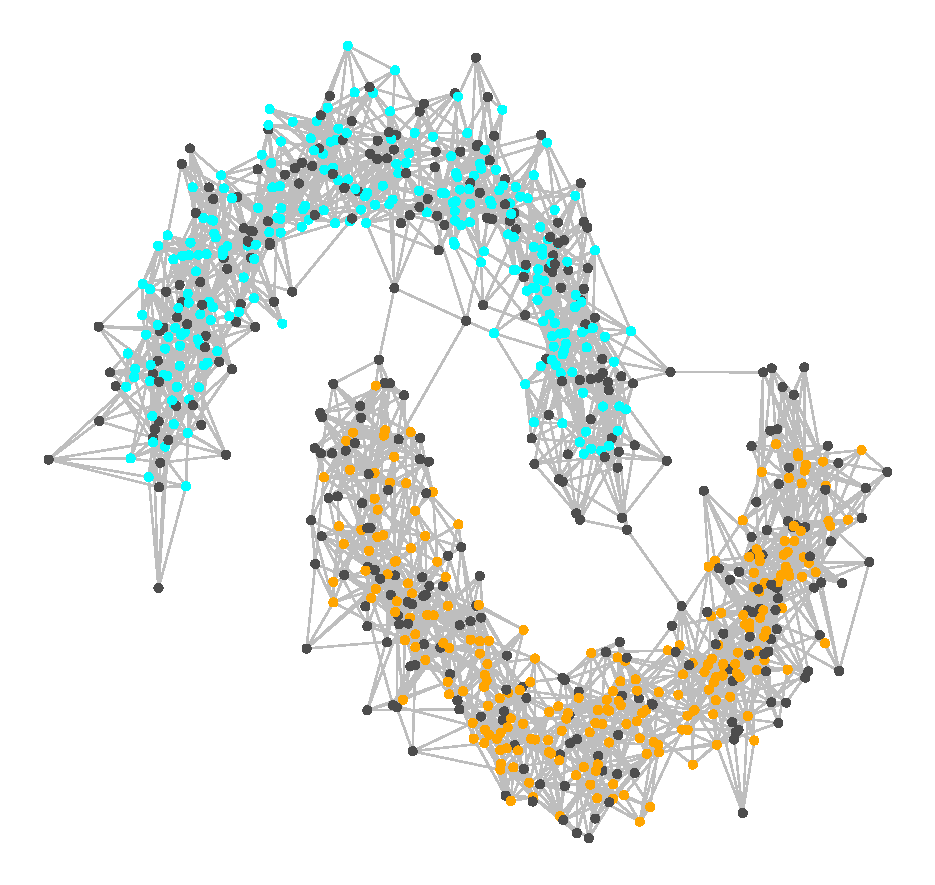
\includegraphics[width=\linewidth]{plots/experiment_2/row4_true_density_cluster}
			\caption{}
		\end{subfigure}
		\begin{subfigure}{.24\linewidth}
			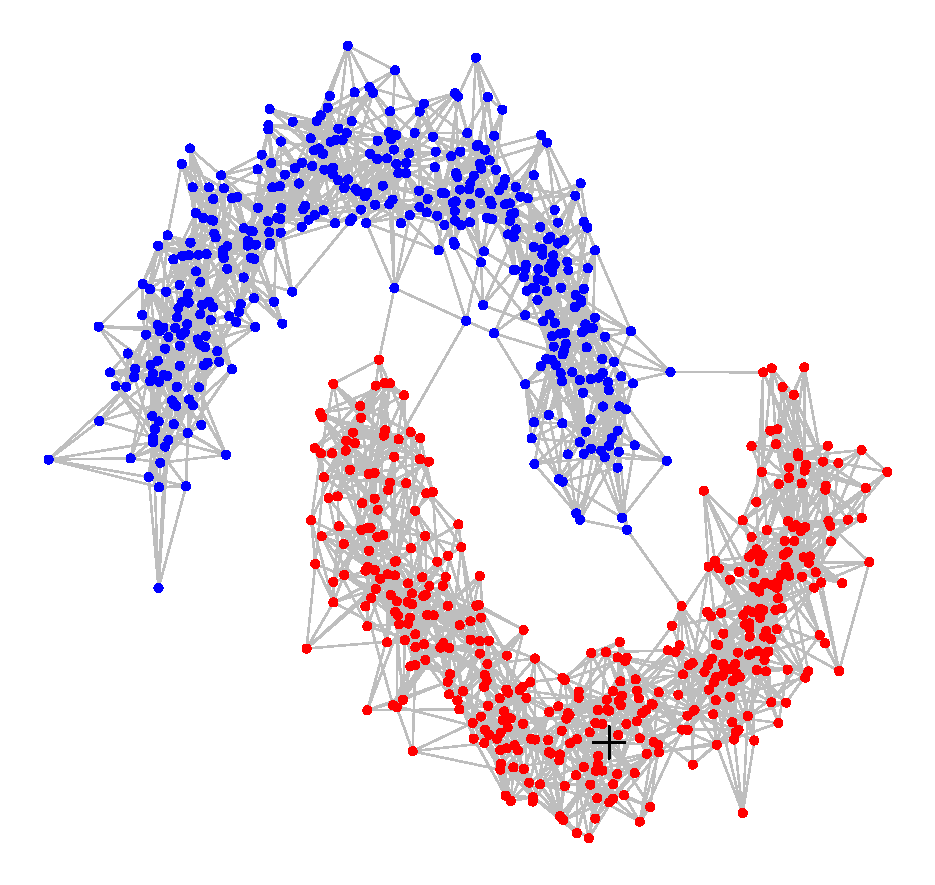
\includegraphics[width=\linewidth]{plots/experiment_2/row4_ppr_cluster}
			\caption{}
		\end{subfigure}
		\begin{subfigure}{.24\linewidth}
			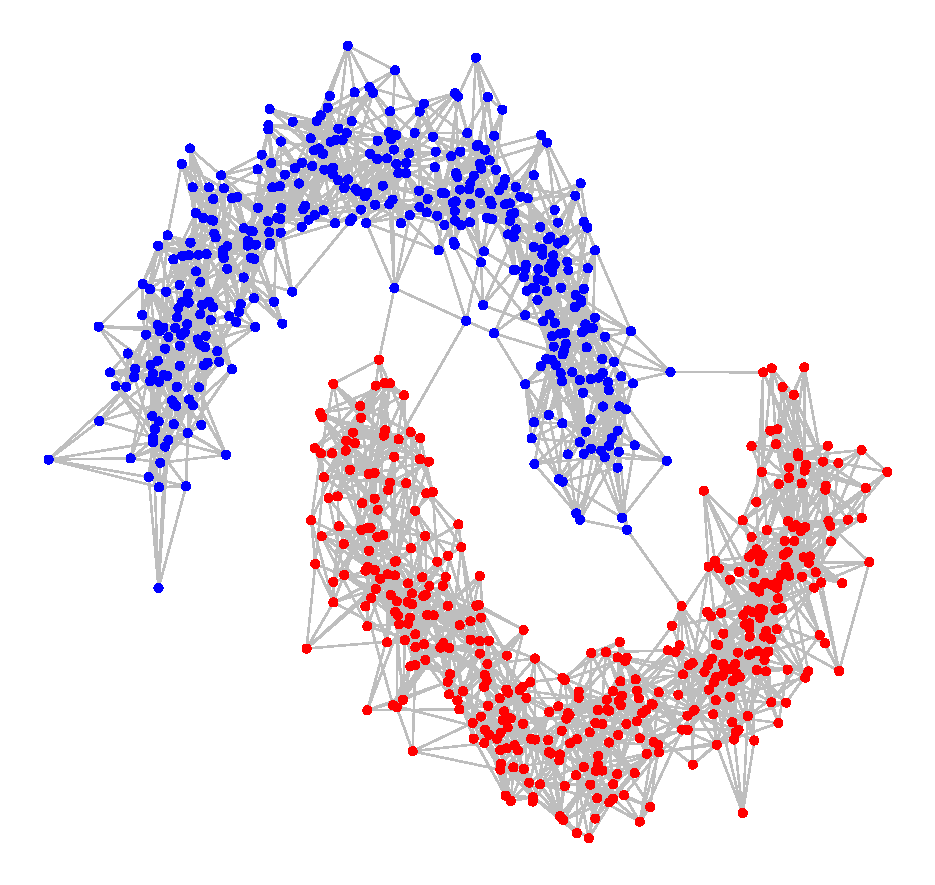
\includegraphics[width=\linewidth]{plots/experiment_2/row4_conductance_cluster}
			\caption{}
		\end{subfigure}
		\begin{subfigure}{.24\linewidth}
			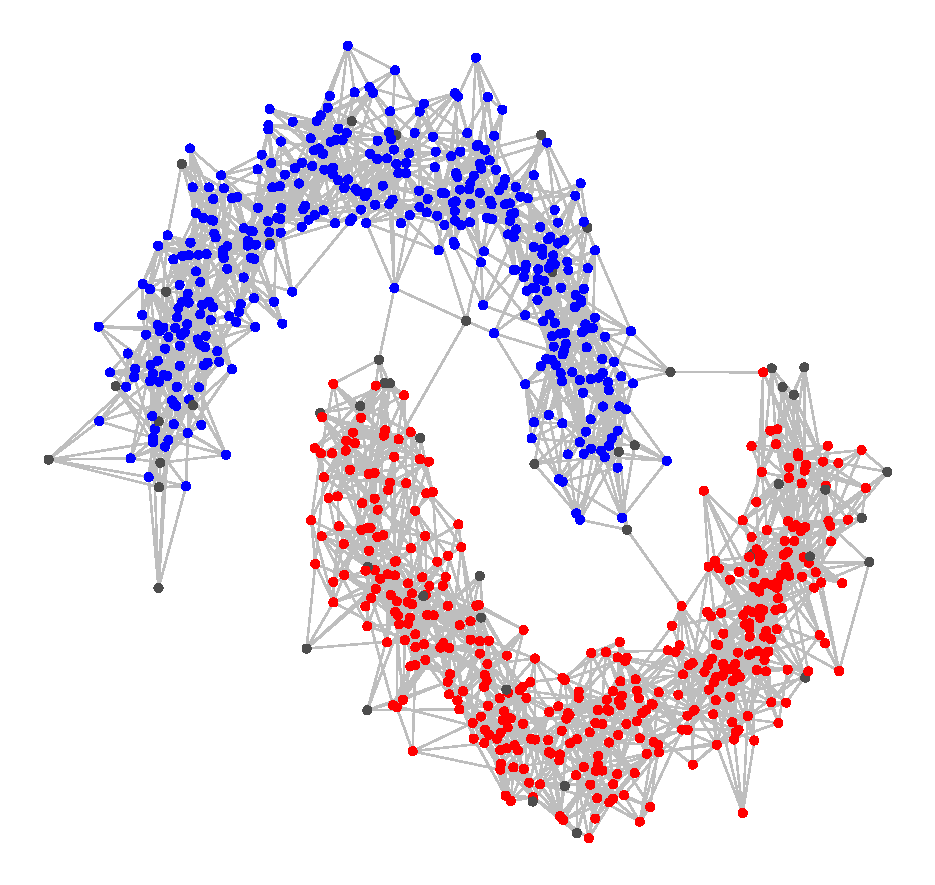
\includegraphics[width=\linewidth]{plots/experiment_2/row4_density_cluster}
			\caption{}
		\end{subfigure}
		\caption{\it\small True density (column 1), PPR (column 2), minimum normalized
			cut (column 3) and estimated density (column 4) clusters for two-moons with 10 dimensional noise. Seed node for PPR denoted by a black cross.} 
		\label{fig:moons_hd}
	\end{adjustbox}
\end{figure}